% ----------------------------------------------------------------
% Book Class (This is a LaTeX2e document)  ***********************
% ----------------------------------------------------------------
\documentclass[11pt,twoside,a4paper]{book}
\usepackage{color}
\usepackage[english]{babel}
\usepackage{amsmath,amsthm}
\usepackage{amsfonts}
\usepackage{hyperref}
%\usepackage[nottoc]{tocbibind}
%\usepackage{natbib}
\usepackage[pdftex]{graphicx}
\usepackage[margin=1.0in]{geometry}
\usepackage{multirow}
\usepackage{listings}
\usepackage{courier}
%\usepackage{makeidx}
\usepackage{multind}
\usepackage{caption}
\usepackage{subcaption}

\lstset{
         basicstyle=\footnotesize\ttfamily, % Standardschrift
         %numbers=left,               % Ort der Zeilennummern
         numberstyle=\tiny,          % Stil der Zeilennummern
         %stepnumber=2,               % Abstand zwischen den Zeilennummern
         numbersep=5pt,              % Abstand der Nummern zum Text
         tabsize=2,                  % Groesse von Tabs
         extendedchars=true,         %
         breaklines=true,            % Zeilen werden Umgebrochen
         keywordstyle=\color{red},
    		frame=b,
 %        keywordstyle=[1]\textbf,    % Stil der Keywords
 %        keywordstyle=[2]\textbf,    %
 %        keywordstyle=[3]\textbf,    %
 %        keywordstyle=[4]\textbf,   \sqrt{\sqrt{}} %
         stringstyle=\color{blue}\ttfamily, % Farbe der String
         showspaces=false,           % Leerzeichen anzeigen ?
         showtabs=false,             % Tabs anzeigen ?
         xleftmargin=17pt,
         framexleftmargin=17pt,
         framexrightmargin=5pt,
         framexbottommargin=4pt,
         %backgroundcolor=\color{lightgray},
         showstringspaces=false      % Leerzeichen in Strings anzeigen ?
         language=Python
 }
 \lstloadlanguages{ Python }
%\DeclareCaptionFont{blue}{\color{blue}}
%\captionsetup[lstlisting]{singlelinecheck=false, labelfont={blue}, textfont={blue}}

\usepackage{caption}
\DeclareCaptionFont{white}{\color{white}}
\DeclareCaptionFormat{listing}{\colorbox[cmyk]{0.43, 0.35, 0.35,0.01}{\parbox{\textwidth}{\hspace{15pt}#1#2#3}}}
\captionsetup[lstlisting]{format=listing,labelfont=white,textfont=white, singlelinecheck=false, margin=0pt, font={bf,footnotesize}}

\usepackage{xr}
\externaldocument{Basics}
\externaldocument{Distributions}
\externaldocument{Relations}
\externaldocument{Models}
\externaldocument{Multivar}

\newcommand{\HRule}{\rule{\linewidth}{0.5mm}}
%\newcommand{\py}[1]{\lstinputlisting[label=py_{#1},caption={#1},language=Python]{../Code/{#1}}}

\makeindex{general}
\makeindex{python}
% \includeonly{Survival}
% ----------------------------------------------------------------
\begin{document}
\begin{titlepage}

\begin{center}


% Upper part of the page
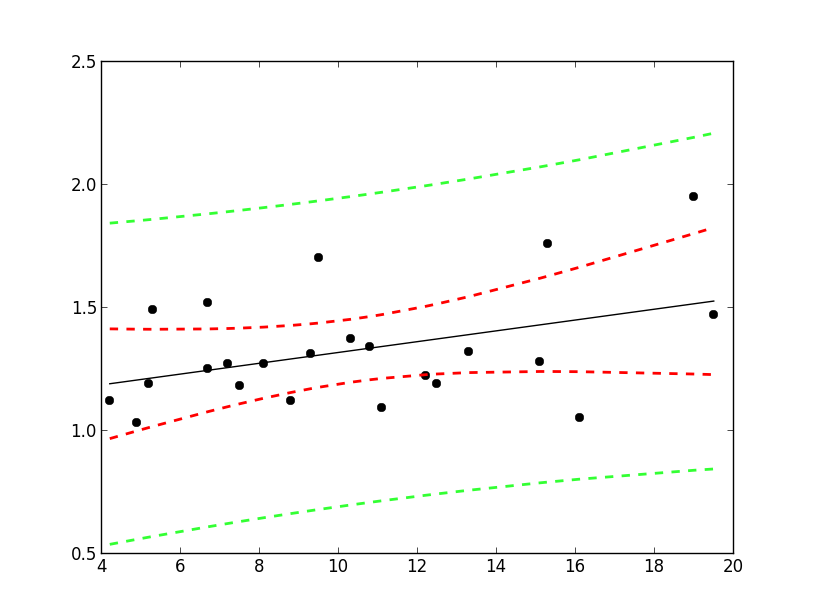
\includegraphics[width=0.5\textwidth]{../Images/regression.png}\\[1cm]

\textsc{\LARGE University of Applied Sciences }\\[1.5cm]

\textsc{\Large An Introduction to}\\[0.5cm]


% Title
\HRule \\[0.4cm]
{ \huge \bfseries Statistics}\\[0.4cm]

\HRule \\[1.5cm]

% Author and supervisor
\begin{minipage}{0.4\textwidth}
\begin{flushleft} \large
\emph{Author:}\\
Thomas \textsc{Haslwanter}
\end{flushleft}
\end{minipage}
\begin{minipage}{0.4\textwidth}
\begin{flushright} \large
\emph{email:} \\
{\small thomas.haslwanter@fh-linz.at}
\end{flushright}
\end{minipage}

\vfill

% Bottom of the page
Version: 2.0 \\
{\large \today} \\[1cm]

\includegraphics[width=1.2cm]{../Images/cc_licence.png}\\
\footnotesize{This work is licensed under a Creative Commons Attribution-NonCommercial 3.0 Unported License.}


\end{center}

\end{titlepage}


\tableofcontents

\chapter{Introduction}

\emph{"Statistics ist the explanation of variance in the light of what remains
unexplained."}

\vspace{5 mm}

Statistics was originally invented - as so many other things - by the famous mathematician C.F. Gauss, who said about his own work \emph{"Ich habe fleissig sein m\"ussen; wer es gleichfalls ist, wird eben so weit kommen"}. Even if your aspirations are not that high, you can get a lot out of statistics. In fact, if your work with real data, you probably won't be able to avoid it. Statistics can

\begin{itemize}
  \item Describe variation.
  \item Make quantitative statements about populations.
  \item Make predictions.
\end{itemize}

\textbf{Books: }There are a number of good books about statistics. My favorite is \cite{altman99}: it does not talk a lot about computers and modeling, but gives you a terrific introduction into the field. Many formulations and examples in this manuscript have been taken from that book. A more modern book, which is more voluminous and in my opionion a bit harder to read, is \cite{Riffenburgh2012}. If you are interested in a simple introduction to modern regression modeling, check out \cite{Kaplan2009}. A very good introduction to “Generalized Linear Models” is \cite{Dobson2008}. If you know your basic statistics, this is a good, advanced starter into statistical modeling.

\vspace{5 mm}

\textbf{WWW: }On the web, you find good very extensive statistics information in English under
\begin{itemize}
    \item \url{http://www.statsref.com/}
    \item \url{http://www.vassarstats.net/}
    \item \url{http://udel.edu/~mcdonald/statintro.html}
    \item \url{http://onlinestatbook.com/2/index.html}
\end{itemize}

 A good German webpage on statistics and regulatory issues is \url{http://www.reiter1.com/}.

\vspace{5 mm}

\textbf{Exercises: }Many examples are already solved in the text. For the use in lectures (or for self-test), additional exercises are provided at the end of most chapters. For lecturers, solutions to these exercises can be provided on demand. Please contact me directly for that via email.

\section{Why Statistics?}

Statistics will help you to
\begin{itemize}
  \item Clarify the question.
  \item Identify the variable and the measure of that variable that will answer that question.
  \item Determine the required sample size.
  \item Find the correct analysis for your data.
  \item Make predictions based on your data.
\end{itemize}

Without statistics, your interpretation of your data can be massively flawed. Take for example the estimated number of German tanks during World War II, also known as the \emph{German tank problem} (\url{http://en.wikipedia.org/wiki/German_tank_problem}): from standard intelligence data, the estimate for the number of German tanks produced per month was $1550$; in contrast, the statistical estimate from the tanks observed led to a number of $327$, which was very close to the actual production number of $342$.

\section{What you should already know}

From previous courses on math, quality control, signal analysis, etc., you are probably already familiar with a number of statistical concepts. While they will be dealt with in detail later on, let me list them here to make sure we start at the same level:

\begin{itemize}
  \item mean
  \item median
  \item mode
  \item standard deviation
  \item variance
  \item confidence intervals
  \item t-test
  \item boxplot
  \item normal distribution
  \item regression coefficient
  \item coefficient of determination
\end{itemize}

\section{Projects}

The biggest problems in statistics do \emph{not} arise from a faulty analysis, but from a faulty experimental design. If you have a suitable topic of interest, you can select to do a project instead of the final exam. For this you will have to

\begin{enumerate}
  \item Read up on the problem.
  \item Design the study:

  \begin{enumerate}
    \item Determine the parameter to analyze.
    \item Decide on the requirements of the sample population.
    \item Plan the randomization.
    \item Decide which test you want to use for the analysis.
  \end{enumerate}

  \item Analyze some data.
  \item Generate the appropriate graphs.
  \item Write up a summary of your project.
\end{enumerate}

\section{Programming Matters}

\subsection{Python}


There are three reasons why I have decided to use Python for this lecture.

\begin{enumerate}
  \item It is the most elegant programming language that I know.
  \item It is free.
  \item It is powerful.
\end{enumerate}

I have not seen many books on Python that I really liked. My favorite introductory book is \cite{Harms2010}.
A good free book, which introduces Python with a focus on statistics, is \href{http://www.kevinsheppard.com/images/0/09/Python_introduction.pdf} {Introduction to Python for Econometrics, Statistics and Data Analysis, by Kevin Sheppard, Oxford University}.

In general, I suggest that you start out by installing a Python distribution which includes the most important libraries. Since I suggest that you use Python $>3.3$ for this course, \cite{pythonxy} (which comes complete with help) is currently not an option, since it is only available for Python 2.7. All the Python packages required for this course are now available for Python 3, so I don't see a good reason to stay with Python 2.7 . My favorites Python 3.3 distributions  are

\begin{enumerate}
    \item \cite{winpython} No admin-rights required.
    \item \cite{anaconda} From Continuum.
\end{enumerate}

which are very good starting points when you are using Windows. \emph{winpython} does not require administrator rights, and \emph{anaconda} is a more recent distribution, which is free for educational purposes.

Mac and Unix users should check out the installations tips from Johansson (see Table \ref{table:python}).

There are also many tutorials available on the internet (Table \ref{table:python}). Personally, most of the time I just google; thereby I stick primarily a) to the official pages, and b) to \url{http://stackoverflow.com/}. Also, I have found user groups surprisingly active and helpful!

\begin{table}

  \footnotesize{
  \centering
   \begin{tabular}{|l p{8 cm}|}
     \hline
     \url{http://scipy-lectures.github.com} & \emph{Python Scientific Lecture Notes.} Pretty comprehensive. \\     \url{http://www.scipy.org/NumPy\_for\_Matlab\_Users} & \emph{NumPy for Matlab Users} Start here if you have Matlab experience. \\
     \url {https://github.com/jrjohansson/scientific-python-lectures} & \emph{Lectures on scientific computing with Python.} Great ipython notebooks! \\     \url{http://docs.python.org/2/tutorial} & \emph{The Python tutorial.} The official introduction. \\
     \url{http://swaroopch.com/notes/python} & \emph{A Byte of Python.} Free book, very good at the introductory level. \\
     \url{http://learnpythonthehardway.org/book/} & \emph{Learn Python the Hard Way, 3rd Ed} A popular, free book that you can work through. \\
     \url{http://www.greenteapress.com/thinkpython} & \emph{ThinkPython.} Free book, for advanced programers. \\

     \hline
   \end{tabular}
   }
  \caption{Python on the WWW}\label{table:python}
\end{table}

If you decide to install things manually, you need the following modules in addition to the Python standard library:

\begin{itemize}
  \item \emph{ipython} ... For interactive work.
  \item \emph{numpy} ... For working with vectors and arrays.
  \item \emph{scipy} ... All the essential scientific algorithms, including those for statistics.
  \item \emph{matplotlib} ... The de-facto standard module for plotting and visualization.
  \item \emph{pandas} ... Adds \emph{DataFrames} (imagine powerful spreadsheets) to Python.
  \item \emph{patsy} ... For working with statistical formulas.
  \item \emph{statsmodels} ... For statistical modeling and advanced analysis.
  \item \emph{seaborn} ... For visualization of statistical data.
\end{itemize}

\subsubsection{Ipython}


Make sure that you have a good programming environment! Currently, my favorite way of programming is similar to my old Matlab style: I first get the individual steps worked out interactively in an \cite{ipython} \emph{qtconsole}. Ipython \index{general}{Python!ipython} provides interactive computing with Python, similar to the commandline in Matlab. It comes with a command history, interactive data visualization, command completion, and a lot of features that make it quick and easy to try out code.
When ipython is started in \emph{pylab mode} (which is the typical configuration), it automatically loads numpy and matplotlib.pyplot into the
active workspace, and provides a very convenient, Matlab-like programing environment. A very helpful new addition is the browser-based \emph{ipython
notebook}, with support for code, text, mathematical expressions, inline plots and other rich media. Please check out the links to the ipython
notebooks in this statistics introduction. I believe that it will  help you to get up to speed with python much more quickly.

And to write a program, I then go to either \emph{Spyder} (which is free) or \emph{Wing} (which is very good, but commercial). \emph{PyCharm} is another IDE with a good debugger, and has very good vim-emulation.

The flexibility of Python has the "disadvantage" that it can come in
different flavors or coding styles. When you know the different approaches,
they are great to use. But when you get started, it can be a bit confusing.
The following section from the Matplotlib documentation may help to clarify
these things:

\subsubsection{Matplotlib, pylab, and pyplot: how are they related?}

\textbf{Matplotlib}\index{general}{Python!Matplotlib} is the whole package; \emph{pylab} is a module in matplotlib that gets installed alongside matplotlib; and \emph{matplotlib.pyplot} is a module in matplotlib.

\textbf{Pyplot}\index{general}{Python!pyplot} provides the state-machine interface to the underlying plotting library in matplotlib. This means that figures and axes are implicitly and automatically created to achieve the desired plot. For example, calling plot from pyplot will automatically create the necessary figure and axes to achieve the desired plot. Setting a title will then automatically set that title to the current axes object:

\begin{lstlisting}
    import matplotlib.pyplot as plt

    plt.plot(arange(10))
    plt.title("Simple Plot")
    plt.show()
\end{lstlisting}

\textbf{Pylab}\index{general}{Python!pylab} combines the pyplot functionality (for plotting) with the numpy functionality (for mathematics and for working with arrays) in a single namespace, making that namespace (or environment) even more MATLAB-like. For example, one can call the sin and cos functions just like you could in MATLAB, as well as having all the features of pyplot.

The pyplot interface is generally preferred for non-interactive plotting (i.e., scripting). The pylab interface is convenient for interactive calculations and plotting, as it minimizes typing. Note that this is what you get if you use the ipython shell with the -pylab option, which imports everything from pylab and makes plotting fully interactive.


\subsubsection{Coding Styles in Python}

In Python you will find different coding styles and usage patterns. These styles are perfectly valid and have their pros and cons. Just about all of the examples can be converted into another style and achieve the same results. The only caveat is to avoid mixing the coding styles for your own code.

Of the different styles, there are two that are officially supported. Therefore, these are the preferred ways to use matplotlib.

For the preferred pyplot style, the imports at the top of your scripts will typically be:

\begin{lstlisting}
    import matplotlib.pyplot as plt
    import numpy as np
\end{lstlisting}

Then one calls, for example, np.arange, np.zeros, np.pi, plt.figure, plt.plot, plt.show, etc. So, a simple example in this style would be:

\begin{lstlisting}
    import matplotlib.pyplot as plt
    import numpy as np
    x = np.arange(0, 10, 0.2)
    y = np.sin(x)
    plt.plot(x, y)
    plt.show()
\end{lstlisting}

Note that this example used pyplot's state-machine to automatically and implicitly create a figure and an axes. For full control of your plots and more advanced usage, use the pyplot interface for creating figures, and then use the object methods for the rest:

\begin{lstlisting}
    import matplotlib.pyplot as plt
    import numpy as np
    x = np.arange(0, 10, 0.2)
    y = np.sin(x)
    fig = plt.figure()
    ax = fig.add_subplot(111)
    ax.plot(x, y)
    plt.show()
\end{lstlisting}

Next, the same example using a pure MATLAB-style:

\begin{lstlisting}
    from pylab import *
    x = arange(0, 10, 0.2)
    y = sin(x)
    plot(x, y)
    show()
\end{lstlisting}

So, why all the extra typing as one moves away from the pure MATLAB-style? For very simple things like this example, the only advantage is academic: the wordier styles are more explicit, more clear as to where things come from and what is going on. For more complicated applications, this explicitness and clarity becomes increasingly valuable, and the richer and more complete object-oriented interface will likely make the program easier to write and maintain.

Here an example, to get you started with Python. For interactive work, it is
simplest to use the \emph{pylab mode}, as shown in the example below. The corresponding ipython
notebook
 \url{http://nbviewer.ipython.org/github/thomas-haslwanter/statsintro/blob/master/ipynb/getting\_started.ipynb})
shows how numpy and matplotlib can be addressed directly. (This is common
practice when writing functions.)

\subsubsection{Example-Session}

\PyImg "gettingStarted.py" (p \pageref{py:gettingStarted_ipy}) gives a short demonstration of Python for scientific data analysis
\index{python}{gettingStarted}


\subsection{Pandas}


\cite{pandas} is a Python module which provides suitable data structures for
statistical analysis. It significantly enhances the abilities of Python for
data input, data organization, and data manipulation. In the following, I assume
that pandas has been imported with

\begin{lstlisting}
    import pandas as pd
\end{lstlisting}

A good introduction to pandas can be found under
\url{http://www.randalolson.com/2012/08/06/statistical-analysis-made-easy-in-python/}

\subsubsection{Data Input}

Pandas offers tools for reading and writing data between in-memory data structures and different
formats, e.g. CSV and text files, Microsoft Excel, and SQL databases. For example, if you have data
in your clipboard, you can import them directly with

\begin{lstlisting}
    data = pd.io.parsers.read_clipboard()
\end{lstlisting}

Or data from "Sheet1" in an Excel-file "data.xls" can be read in easily with

\begin{lstlisting}
    xls = pd.io.parsers.ExcelFile('data.xls')
    data = xls.parse('Sheet1')
\end{lstlisting}

\textbf{Example: }
\PyImg "readZip.py" (p \pageref{py:readZip}) This advanced script shows you how you can directly import data from an MS-Excel file from a zipped archive on the web.
\index{python}{readZip}

\subsubsection{Data Handling and Manipulation}
Pandas offers powerful functions to handle missing data and "nans", and other kinds of data manipulation like pivoting.

To handle labeled data, pandas introduces \emph{DataFrame} objects. A DataFrame is a 2-dimensional labeled data structure with columns of potentially different types. You can think of it like a spreadsheet or SQL table. It is generally the most commonly used pandas object. For example, you can use data-frames to efficiently group objects, and do a statistical evaluation of each group:

\begin{lstlisting}
    x = tile([1,2,3], 4)
    y = randn(len(x))
    df = pd.DataFrame({'treatment':x, 'result':y})
    groups = df.groupby('treatment')
    print(groups['result'].describe())
\end{lstlisting}

produces

\begin{lstlisting}
     treatment
    1          count    4.000000
               mean    -1.693818
               std      1.559007
               min     -3.857303
               25%     -2.293582
               50%     -1.279452
               75%     -0.679688
               max     -0.359065
    2          count    4.000000
               mean    -0.240799
               std      0.610826
               min     -0.780429
               25%     -0.563200
               50%     -0.406580
               75%     -0.084178
               max      0.630393
    3          count    4.000000
               mean     0.177045
               std      0.703775
               min     -0.298325
               25%     -0.255564
               50%     -0.101432
               75%      0.331177
               max      1.209367
    dtype: float64
\end{lstlisting}

For statistical analysis, pandas becomes really powerful if you combine it with \emph{statsmodels} (see below).

\PyImg "pandasIntro.py" (p \pageref{py:pandasIntro}) shows you how pandas can be used for data analysis.
\index{python}{pandasIntro}

\subsection{Statsmodels}

\cite{statsmodels} is a Python module that provides classes and functions for the estimation of many different statistical models, as well as for conducting statistical tests, and statistical data exploration. An extensive list of result statistics are available for each estimator. In its latest release (version 0.5), statsmodels also allows the formulation of models with the popular formula language also used by $R$, the leading statistics package. For example, data on the connection between academic "success", "intelligence" and "diligence" can be described with the model $success ~ intelligence * diligence$, which would capture the direct effect of "intelligence" and "diligence", as well as the interaction. You find more information on that topic in the section "Statistical Models".

While for complex statistical models R still has an edge, python has a much clearer and more readable syntax, and is arguably more powerful for the data manipulation often required for statistical analysis.

\subsection{Seaborn}

\cite{seaborn} is a Python visualization library based on matplotlib. Its primary goal is to provide a concise, high-level interface for drawing statistical graphics that are both informative and attractive.

\begin{lstlisting}
        x = linspace(1, 7, 50)
        y = 3 + 2*x + 1.5*randn(len(x))
        sns.regplot(x,y)
\end{lstlisting}

already produces a nice and informative regression plot

\begin{figure}[ht]
  \centering
  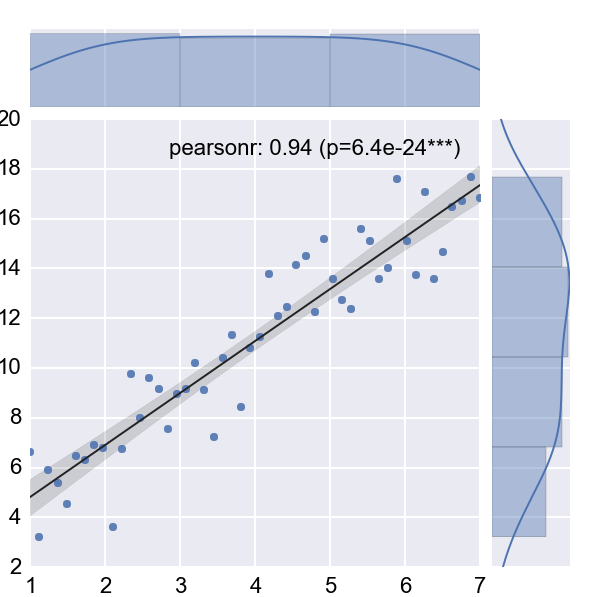
\includegraphics[width=0.5\textwidth]{../Images/regplot.png}\\
  \caption{Regression plot, from \emph{seaborn}, with a substantial amount of added information.}
\end{figure}

\subsection{General Routines}
Here is also a good place to introduce the short function that we will use a number of times to simplify the reading in of data:

\PyImg "getData.py" (p \pageref{py:getData}) Gets the input data for the Python programs in this script.
\index{python}{getData}

\section{Exercises}

\begin{itemize}
  \item Read in data from different sources:
  \begin{itemize}
    \item A CVS-file with a header ('Data\textbackslash Swimming\textbackslash swimming\_100m.csv')
    \item An MS-Excel file ('Data\textbackslash data\_dobson\textbackslash GLM\_data\textbackslash Table 2.8 Waist loss.xls')
    \item Data from the WWW (see "readZip.py" \ref{py:readZip})
  \end{itemize}
  \item
  \begin{itemize}
      \item Generate a pandas dataframe, with the x-column time stamps from 0 to 10 sec, at a rate of 10 Hz, the y-column data values with a sine with 1.5 Hz, and the z-column the corresponding cosine values. Label the x-column "Xvals", and the y-column "YVals", and the z-column "ZVals".
      \item Show the head of this dataframe
      \item Extract the data in lines 10-15 from "Yvals" and "ZVals", and write them to the file "out.txt".
  \end{itemize}
\end{itemize}

\chapter{Basic Principles}

\section{Datatypes}

The type of your data is essential for the choice of test that you have to use for your data analysis. Your data can have one of the following datatypes:

\subsection{Categorical} \index{general}{data!categorical}

\subsubsection{boolean}
Some data can only have two values. For example,
\begin{enumerate}
  \item male/female
  \item smoker/non-smoker
\end{enumerate}

\subsubsection{nominal}\index{general}{nominal}
Many classifications require more than two categories, e.g. \emph{married / single / divorced}

\subsubsection{ordinal}\index{general}{data!ordinal}
These are ordered categorical data, e.g. \emph{very few / few / some / many / very many}

\subsection{Numerical}\index{general}{data!numerical}

\subsubsection{Numerical discrete}
For example \emph{Number of children: 0 1 2 3 4 5}

\subsubsection{Numerical continuous}
Whenever possible, it is best to record the data in their original continuous format, and only with a sensible number of decimal places. For example, it does not make sense to record the body size with more than 1 mm accuracy, as there are larger changes in body height between the size in the morning and the size in the evening, due to compression of the intervertebral disks.

\section{Data Display}

When working with a statistical data set, you should \emph{always} first look at the raw-data. Our visual system is incredibly good at recognizing patterns in visually represented data. The programs used for making the plots presented here can be found in "figsBasicPrinciples.py" (p \pageref{py:BasicPrinciples}). For data visualization, check out the Python package \href{http://www.stanford.edu/~mwaskom/software/seaborn/} {seaborn}, which aims to provide a concise, high-level interface for drawing statistical graphics that are both informative and attractive.

\subsection{Scatter Plots}\index{general}{plots!scatter}

This is the simplest way of representing your data: just plot each individual data point. (In cases where many data points are superposed, you may want to add a little bit of jitter to show each data point.)

\begin{figure}[h]
  \centering
  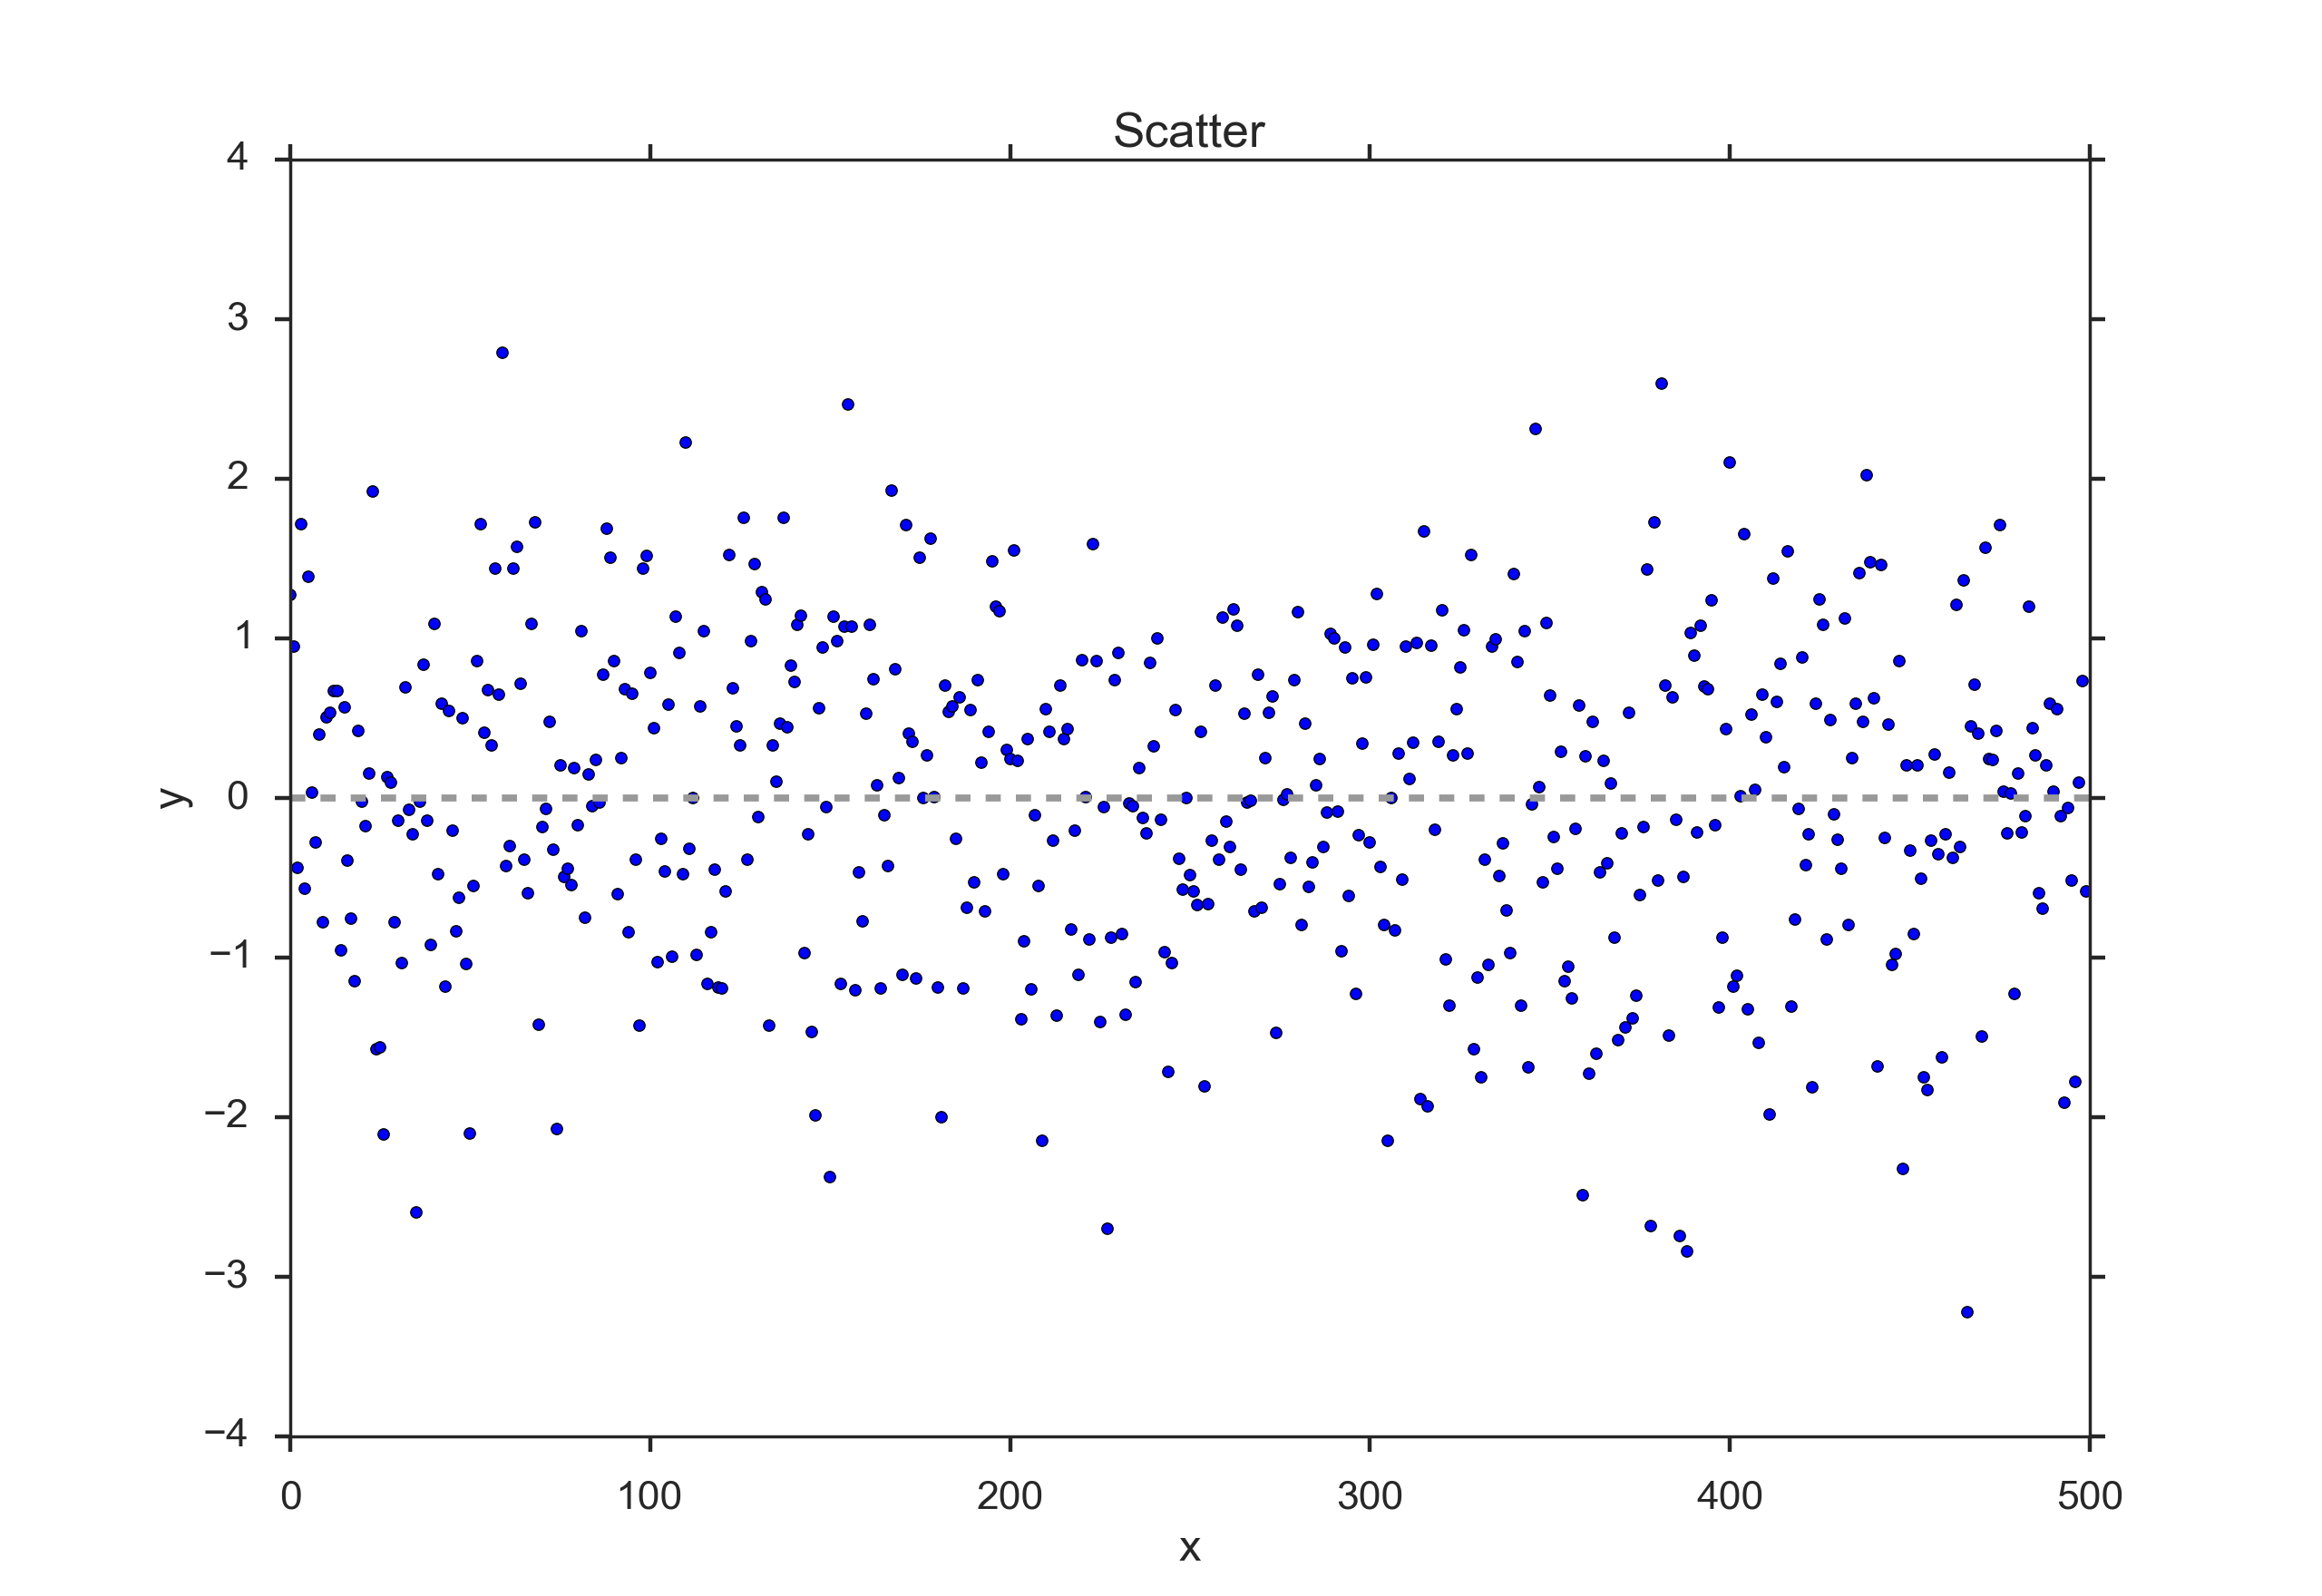
\includegraphics[width=0.5\textwidth]{../Images/scatterPlot.png}\\
  \caption{Scatter plot}
\end{figure}

\subsection{Histograms}\index{general}{plots!histogram}


\emph{Histograms} provide a first good overview of the distribution of your data.
If you divide by the overall number of data points, you get a \emph{relative frequency
histogram}; and if you just connect the top center points of each bin, you obtain a
\emph{relative frequency polygon}.

You can also smooth histograms with \emph{kernel-density-estimations (kde-plots)}. Those are nicely implemented and described in \emph{seaborn}.

\begin{figure}[ht]
  \centering
  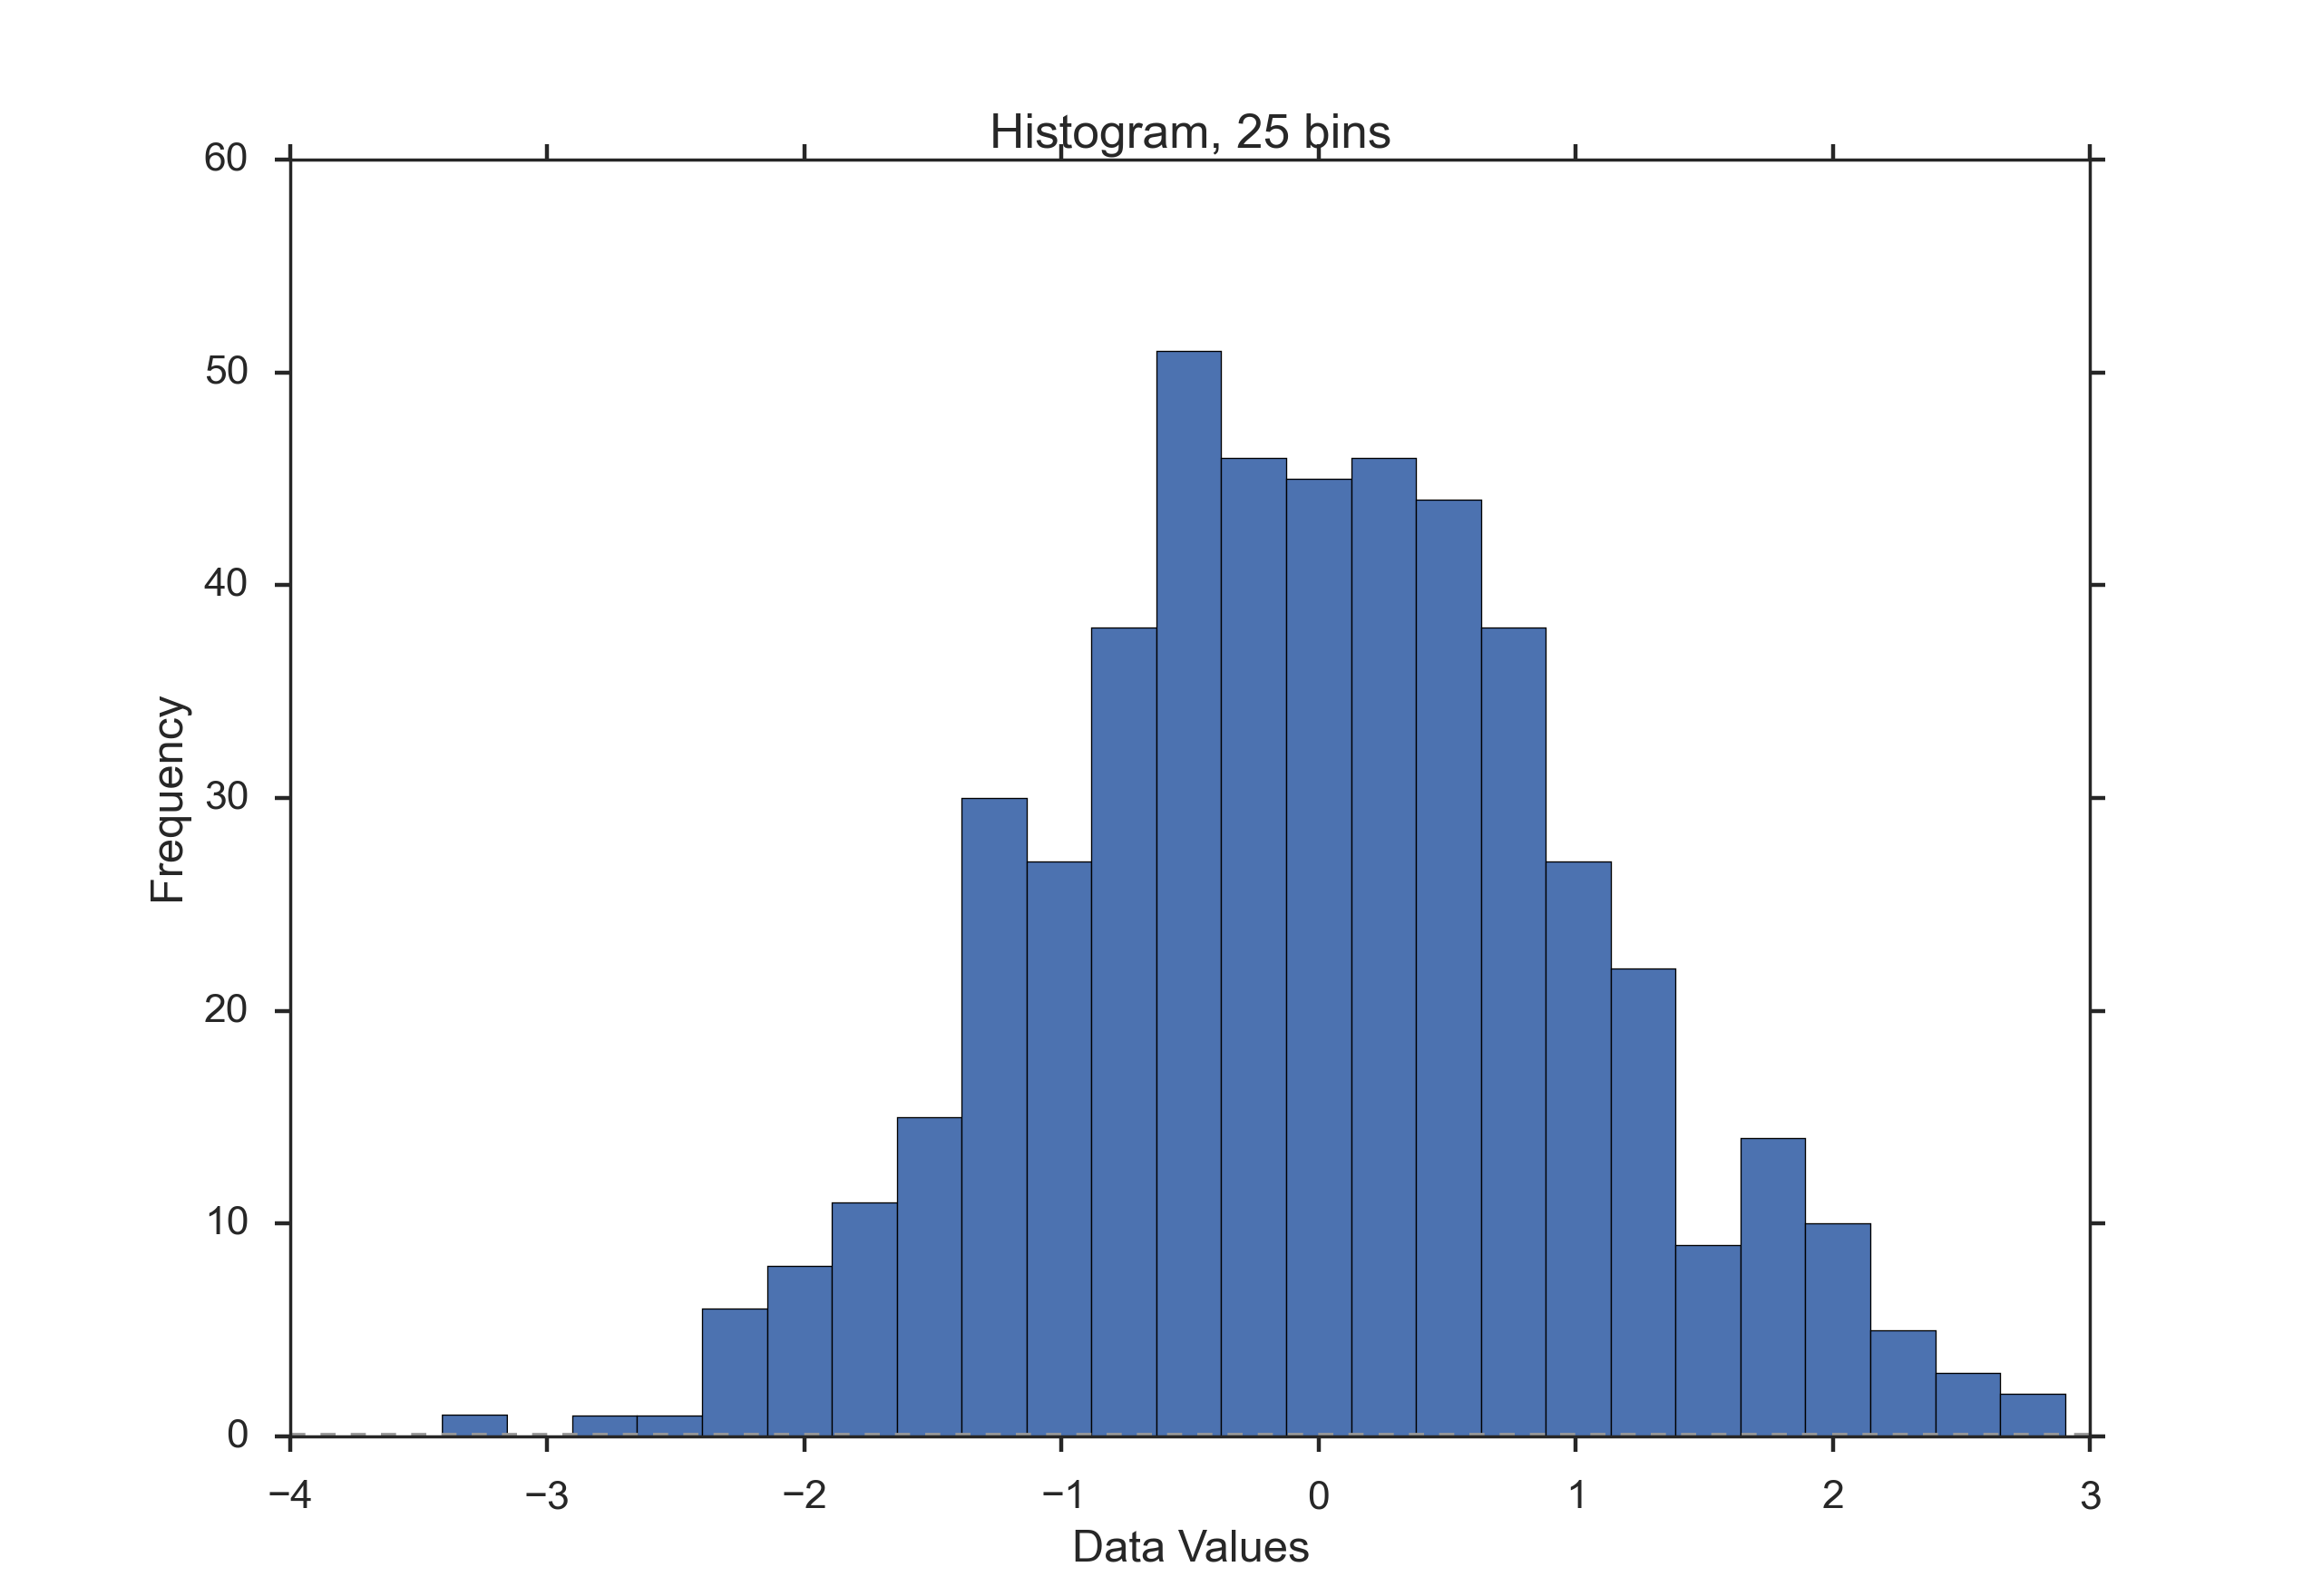
\includegraphics[width=0.5\textwidth]{../Images/Histogram.png}\\
  \caption{Histogram}
\end{figure}

\subsection{KDE-plots}\index{general}{plots!kde}

\footnote{This paragraph is taken from Wikipedia, "Kernel density estimation".} Kernel density estimates are closely related to histograms, but can be endowed with properties such as smoothness or continuity by using a suitable kernel. To see this, we compare the construction of histogram and kernel density estimators, using these 6 data points: x1 = −2.1, x2 = −1.3, x3 = −0.4, x4 = 1.9, x5 = 5.1, x6 = 6.2. For the histogram, first the horizontal axis is divided into sub-intervals or bins which cover the range of the data. In this case, we have 6 bins each of width 2. Whenever a data point falls inside this interval, we place a box of height 1/12. If more than one data point falls inside the same bin, we stack the boxes on top of each other.

For the kernel density estimate, we place a normal kernel with variance 2.25 (indicated by the red dashed lines) on each of the data points xi. The kernels are summed to make the kernel density estimate (solid blue curve). The smoothness of the kernel density estimate is evident compared to the discreteness of the histogram, as kernel density estimates converge faster to the true underlying density for continuous random variables.

\begin{figure}[ht]
  \centering
  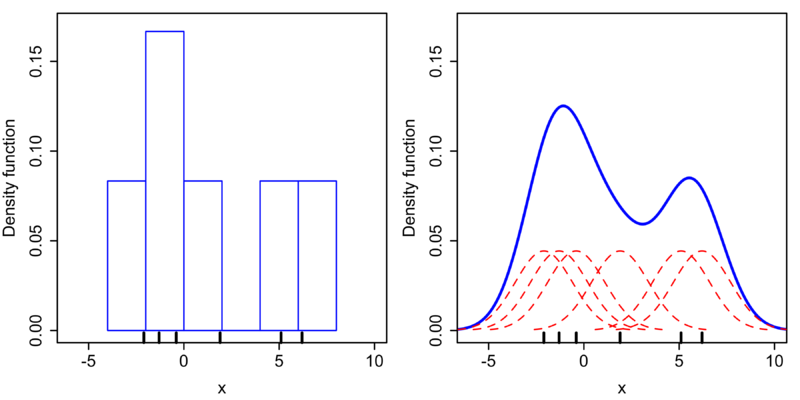
\includegraphics[width=0.75\textwidth]{../Images/Comparison_of_1D_histogram_and_KDE.png}\\
  \caption{Comparison of the histogram (left) and kernel density estimate (right) constructed using the same data. The 6 individual kernels are the red dashed curves, the kernel density estimate the blue curves. The data points are the rug plot on the horizontal axis. (from Wikipedia)}
\end{figure}

The bandwidth of the kernel is a free parameter which exhibits a strong influence on the resulting estimate. To illustrate its effect, we take a simulated random sample from the standard normal distribution (plotted at the blue spikes in the rug plot on the horizontal axis). The grey curve is the true density (a normal density with mean 0 and variance 1). In comparison, the red curve is undersmoothed since it contains too many spurious data artifacts arising from using a bandwidth h = 0.05 which is too small. The green curve is oversmoothed since using the bandwidth h = 2 obscures much of the underlying structure. The black curve with a bandwidth of h = 0.337 is considered to be optimally smoothed since its density estimate is close to the true density.

\begin{figure}[ht]
  \centering
  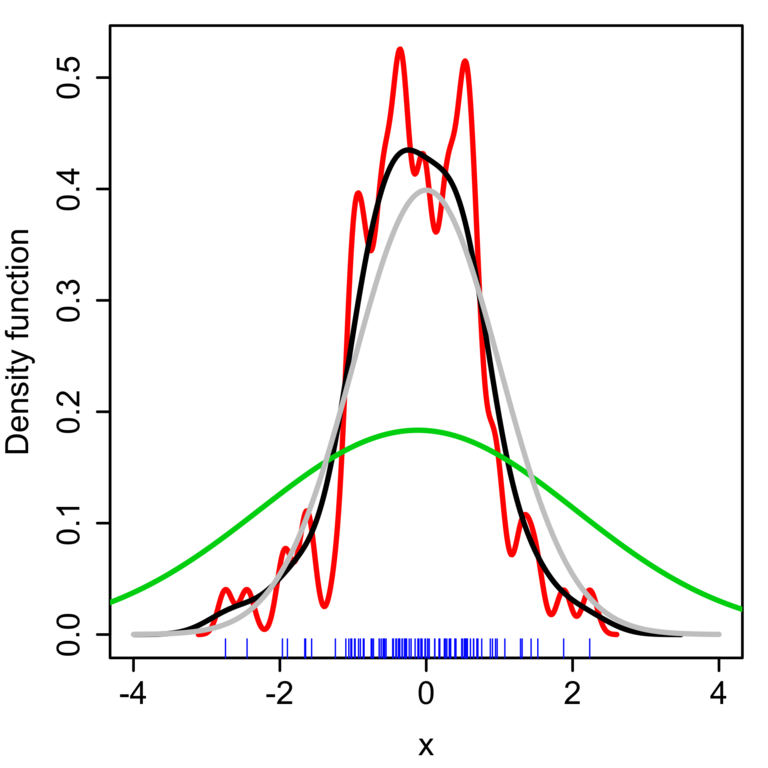
\includegraphics[width=0.5\textwidth]{../Images/Comparison_of_1D_bandwidth_selectors.png}\\
  \caption{Kernel density estimate (KDE) with different bandwidths of a random sample of 100 points from a standard normal distribution. Grey: true density (standard normal). Red: KDE with h=0.05. Green: KDE with h=2. Black: KDE with h=0.337. (from Wikipedia)}
\end{figure}

It can be shown that under certain conditions the optimal choice for h is
\begin{equation}
  h = \left(\frac{4\hat{\sigma}^5}{3n}\right)^{\frac{1}{5}} \approx 1.06 \hat{\sigma} n^{-1/5},
\end{equation}


where $\hat{\sigma}$ is the standard deviation of the samples.


\subsection{Cumulative Frequencies}\index{general}{cumulative frequency}

\emph{Cumulative frequency} curves indicate the number (or percent) of data with less than a given value. This is important for the statistical analysis (e.g. when we want to know the data range containing 95\% of all the values). Cumulative frequencies
are also useful for comparing the distribution of values in two or more different groups of individuals.

When you use percentage points, the cumulative frequency presentation has the additional advantage that it is bounded:

\begin{equation*}
  0 \leq x \leq 1
\end{equation*}

\begin{figure}[ht]
  \centering
  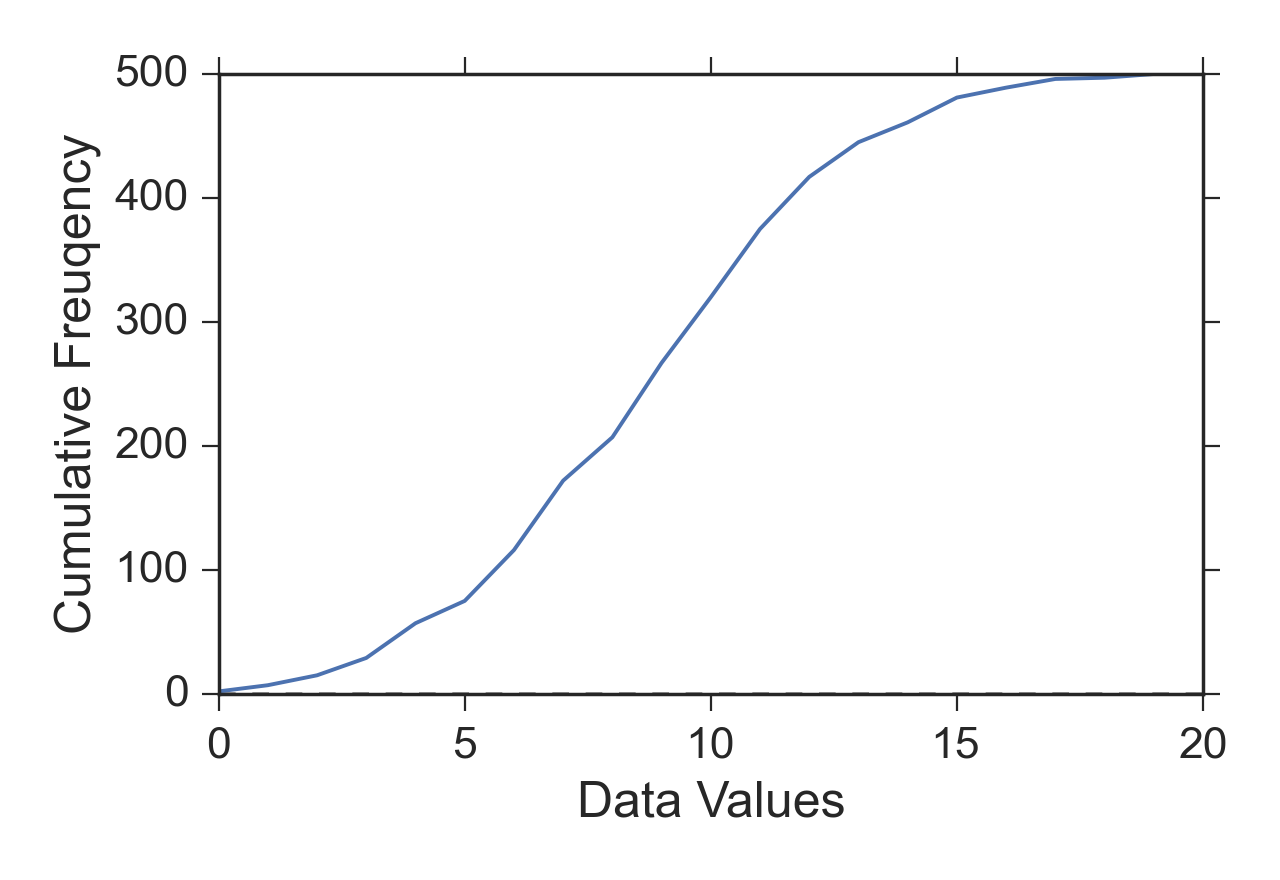
\includegraphics[width=0.5\textwidth]{../Images/CumulativeFrequencyFunction.png}\\
  \caption{Cumulative frequency function}
\end{figure}

\subsection{Box Plots}\index{general}{plots!boxplot}

\emph{Box plots} are frequently used in scientific publications to indicate values in two or more groups. The error bars typically indicate the \emph{range}. However, outliers are often excluded, and plotted separately. There are a number of tests to check for outliers. One of them is to check for data which lie more than 1.5 * \emph{inter-quartile-range} (IQR) above or below the first/third quartile (see Section \ref{sec:centiles}).

\begin{figure}[!ht]
  \centering
  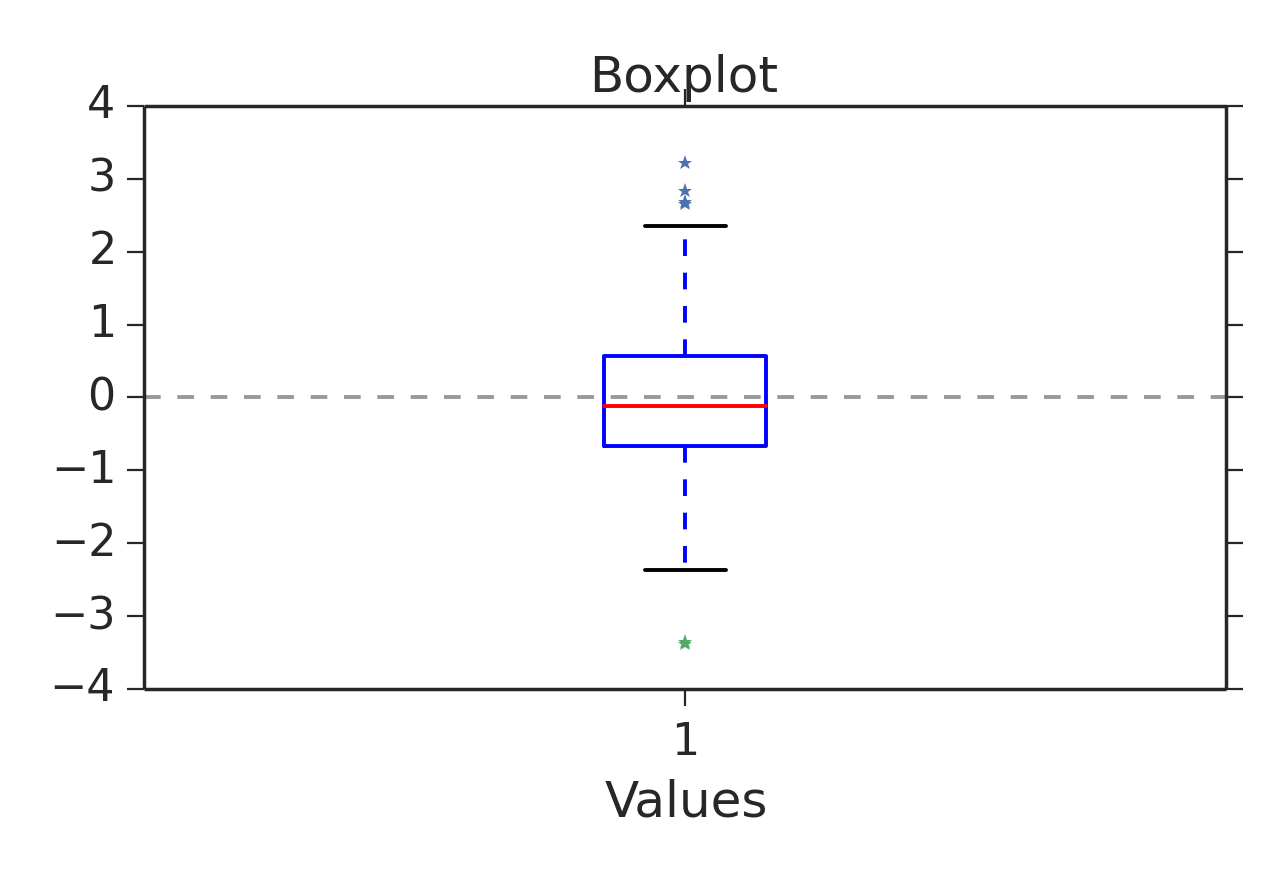
\includegraphics[width=0.5\textwidth]{../Images/boxplot.png}\\
  \caption{Box plot}\label{fig:Boxplot}
\end{figure}

Boxplots are often combined with KDE-plots to produce so-called \emph{violin-plots} \index{general}{plots!violinplot}, as shown in Figure \ref{fig:violin}.

\begin{figure}
  \centering
  % Requires \usepackage{graphicx}
  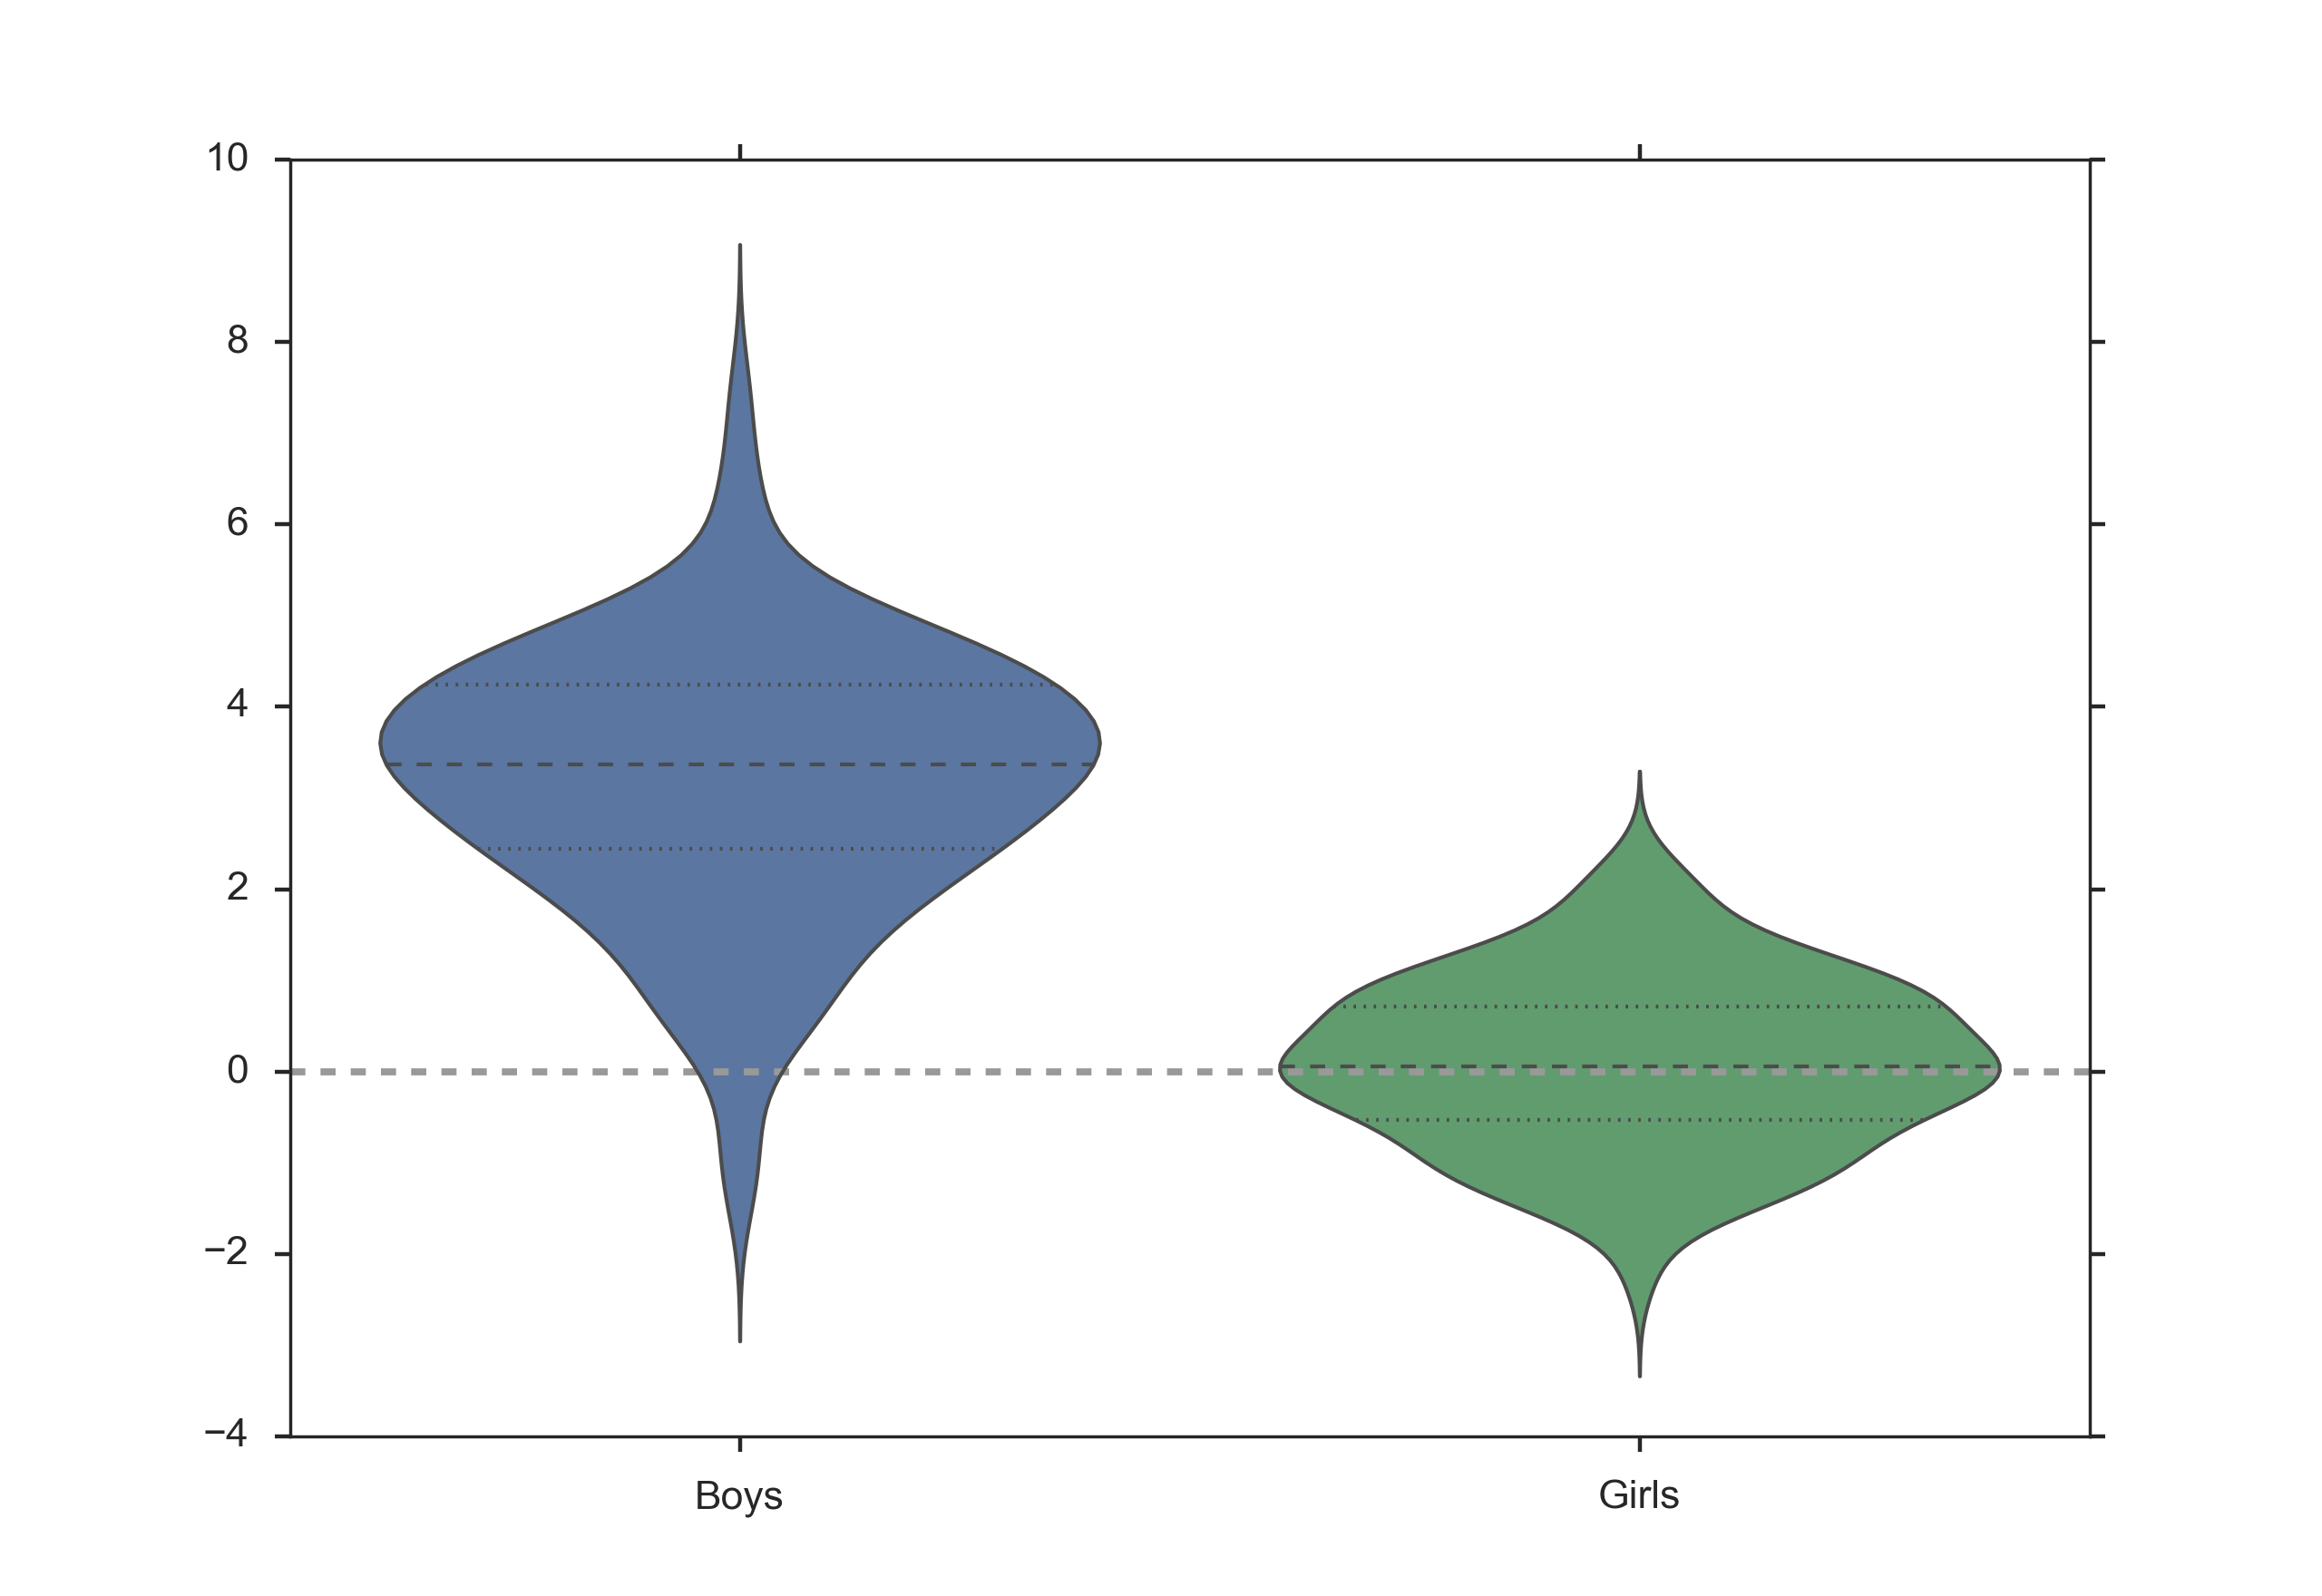
\includegraphics[width=0.75\textwidth]{../Images/violinplot.png}\\
  \caption{Violinplot, produced with \emph{seaborn}.}\label{fig:violin}
\end{figure}

\subsection{Programs: Data Display}
\PyImg "figsBasicPrinciples.py" (p \pageref{py:BasicPrinciples}) shows how the plots in this section have been generated.
\index{python}{figsBasicPrinciples}

\section{Study Design}


\subsection{Types of Studies}

\subsubsection{Observational or experimental}
With \emph{observational} studies the researcher only collects information, but does not interact with the study population. In contrast, in \emph{experimental} studies the researcher deliberately influences events (e.g. treats the patient with a new type of treatment) and investigates the effects of these interventions.

\subsubsection{Prospective or retrospective}
In \emph{prospective} studies the data are collected, starting with the beginning of the study. In contrast, a \emph{retrospective} study takes data acquired from previous events, e.g. routine tests taken at a hospital.

\subsubsection{Longitudinal or cross-sectional}
In \emph{longitudinal} investigations, the researcher collects information over a period of time, maybe multiple times from each patient. In contrast, in \emph{cross-sectional} studies individuals are observed only once. For example, most surveys are cross-sectional, but experiments are usually longitudinal.

\subsubsection{Case control and Cohort studies}
In \emph{case control} studies, first the patients are treated, and then they are selected for inclusion in the study, based on some characteristic (e.g. if they responded to a certain medication). In contrast, in \emph{cohort studies}, first subjects of interest are selected, and then these subjects are studied over time, e.g. for their response to a treatment.

\subsection{Design of Experiments}

\subsubsection{Bias} \index{general}{bias}
In general, when selecting our subject you try to make them representative of the population that you want to study; and you try to conduct your experiments in a way representative of investigations by other researchers. However, it is \emph{very} easy to get a \emph{bias} into your data. Bias can arise from a number of sources:
\begin{itemize}
  \item The selection of subjects.
  \item The structure of the experiment.
  \item The measurement device.
  \item The analysis of the data.
\end{itemize}
Care should be taken to avoid bias as much as possible.

\subsubsection{Randomized controlled trial} \index{general}{randomized controlled trial}
The gold standard for experimental scientific clinical trials is the \emph{randomized controlled trial}. Thereby bias is avoided by splitting the subjects to be tested into an \emph{intervention group} and a \emph{control group}\index{general}{control group}. The group allocation is made \emph{random}. By having the groups differ in only one aspect, i.e. is the factor \emph{treatment}, we should be able to detect the effect of the treatment on the patients.
Factors that can affect the outcome of the experiment are called \emph{covariates} or \emph{confoundings}. Through \emph{randomization}, covariates should be balanced across the groups.

\subsubsection{Randomization} \index{general}{randomization}
This may be one of the most important aspects of experimental planning. Randomization is used to avoid bias as much as possible, and there are different ways to randomize an experiment. For the randomization, \emph{random number generators}, which are available with most computer languages, can be used. To minimize the chance of bias, the randomly allocated numbers should be presented to the experimenter as late as possible.

Depending on the experiment, there are different ways to randomize the group assignment.

\paragraph{Simple randomization}
This procedure is robust against selection and accidental bias. The disadvantage is that the resulting groupsize can differ significantly.

For many types of data analysis it is important to have the same sample number in each group. To achieve this, other options are possible:

\paragraph{Block randomization}
This is used to keep the number of subjects in the different groups closely balanced at all times. For example, if you have two types of treatment, A and B, you can allocate them to two subjects in the following blocks:

\begin{enumerate}
  \item AABB
  \item ABAB
  \item ABBA
  \item BBAA
  \item BABA
  \item BAAB
\end{enumerate}

Based on this, you can use a random number generator to generate random integers between 1 and 6, and use the corresponding blocks to allocate the respective treatments. This will keep the number of subjects in each group always almost equal.

\paragraph{Minimization}
A closely related, but not completely random way to allocate a treatment is \emph{minimization}. Thereby you take whichever treatment has the smallest number of subjects, and allocate this treatment with a probability greater than 0.5 to the next patient.

\paragraph{Stratified randomization}
Sometimes you may want to include a wider variety of subjects, with different characteristics. For example, you may choose to have younger as well as older subjects. In that case you should try to keep the number of subjects within each \emph{stratum} balanced. For this you will have to keep different lists of random numbers for each group of subjects.

\subsubsection{Crossover studies} \index{general}{crossover studies}
An alternative to randomization is the \emph{crossover} design of studies. A crossover study is a longitudinal study in which subjects receive a sequence of different treatments. Every subject receives every treatment. To avoid causal effects, the sequence of the treatment allocation should be randomized.

\subsubsection{Blinding} \index{general}{blinding}
Consciously or not, the experimenter can significantly influence the outcome of an experiment. For example, a young researcher with a new "brilliant" idea for a new treatment will be bias in the execution of the experiment, as well in the analysis of the data, to see his hypothesis confirmed. To avoid such a subjective influence, ideally the experimenter as well as the subject should be blinded to the therapy. This is referred to as \emph{double blinding}. If also the person who does the analysis does not know which group the subject has been allocated to, we speak about \emph{triple blinding}.

\subsubsection{Replication} \index{general}{replication}
For variable measurements it is helpful to have a number of independent repetitions of each measurement.

\subsubsection{Sample selection} \index{general}{sample selection}
When selecting your subjects, you should take care of two points:

\begin{enumerate}
  \item Make sure that the samples are representative of the population.
  \item In comparative studies, care is needed in making groups similar with respect to known sources of variation.
\end{enumerate}

For example, if you select your subjects randomly from patients at a hospital, you automatically bias your sample towards subjects with health problems.

\subsubsection{Sample size}
Many studies fail, because the sample size is too small to observed an effect of the desired magnitude. To plan your sample size, you have to know
\begin{itemize}
  \item What is the variance of the parameter in the population you are investigating.
  \item What is the magnitude of the effect you are interested in, relative to the standard deviation of the parameter.
\end{itemize}

\subsection{Structure of Experiments}


In a designed experiment, there may be several conditions, called \emph{factors}\index{general}{factor}, that are controlled by the experimenter. If each combination of factors is tested, we talk about a \emph{factorial design} of the experiment.

In planning the analysis, you have to keep the important distinction between \emph{within subject} comparisons, and \emph{between subjects} comparisons.

%(Lecture 3)

\subsection{Data Management}

\subsubsection{Documentation} \index{general}{documentation}
Make sure that you document all the factors that may influence your results:

\begin{itemize}
  \item The date and time of the experiment.
  \item Information about the experimenters and the subjects.
  \item The exact paradigm that you have decided on.
  \item Anything noteworthy that happens during the experiment.
\end{itemize}

\subsubsection{Data Handling}
You can already significantly facilitate the data handling by storing your data with telltale names. For example, if you execute your experiments in Vienna and in Linz, you can store your rawdata with the format "[town][year][month][day].dat". For example, an experiment in Vienna on April 1, 2013 would be stored as "vi20130401.dat".

When you have finished recording the data, back up your data right away. Best do that into a directory that is separate from the one where you do your data analysis afterwards.

\subsection{Clinical Investigation Plan}

To design a medical study properly is not only advisable - it is even required by ISO 14155-1:2003, for \emph{Clinical investigations of medical devices for human subjects}. This norm specifies many aspects of your clinical study. It enforces the preparation of a \emph{Clinical Investigation Plan (CIP)}, specifying

\begin{enumerate}
  \item Type of study (e.g. double-blind, with or without control group etc.).
  \item Discussion of the control group and the allocation procedure.
  \item Description of the paradigm.
  \item Description and justification of primary endpoint of study.
  \item Description and justification of chosen measurement variable.
  \item Measurement devices and their calibration.
  \item Inclusion criteria for subjects.
  \item Exclusion criteria for subjects.
  \item Point of inclusion ("When is a subject part of the study?")
  \item Description of the measurement procedure.
  \item Criteria and procedures for the dropout of a subject.
  \item Chosen sample number and level of significance, and their justification.
  \item Procedure for documentation of negative effects or side-effects.
  \item List of factors that can influence the measurement results or their interpretation.
  \item Procedure for documentation, also for missing data.
  \item Statistical analysis procedure.
  \item The designation of a \emph{monitor} for the investigation.
  \item The designation of a \emph{clinical investigator}.
  \item Specification the data handling.
\end{enumerate}

\section{Exercises}

\begin{enumerate}
  \item
  \begin{enumerate}
    \item Read in the data from 'Data\textbackslash amst\textbackslash babyboom.dat.txt'.
    \item Inspect them visually, and give a numerical description of the data.
    \item Are the data normally distributed?
    \item How would you design the corresponding study?
  \end{enumerate}

\end{enumerate}



\chapter{Distributions of one Variable}


\section{Characterizing a Distribution}

\subsection{Population and samples}

While the whole \emph{population} of a group has certain characteristics,
we can typically never measure all of them. In many cases, the population distribution
is described by an idealized, continuous distribution function.

In the analysis of measured data, in contrast, we have to confine
ourselves to investigate a (hopefully representative) \emph{sample} of this group, and
estimate the properties of the population from this sample.

\subsection{Continuous Distribution Functions}

A continuous distribution function describes the distribution of a population, and can be represented in several equivalent ways:

\subsubsection{Probability Density Function (PDF)}\index{general}{probability density function}
The PDF, or density of a continuous random variable, is a function that describes the relative likelihood for a random variable $X$ to take on a given value $x$.
In the mathematical fields of probability and statistics, a \emph{random variate x} \index{general}{random variate} is a particular outcome of a \emph{random variable X}: the random variates which are other outcomes of the same random variable might have different values.

Since the likelihood to find any given value cannot be less than zero, and since the variable has to have some value, the PDF has the following properties:

\begin{itemize}
  \item $PDF(x) \geq 0\,\forall \,x \in \mathbb{R}$
  \item $ \int\limits_{ - \infty }^\infty  {PDF(x)dx = 1} $
\end{itemize}

\begin{figure}
  \centering
  % Requires \usepackage{graphicx}
  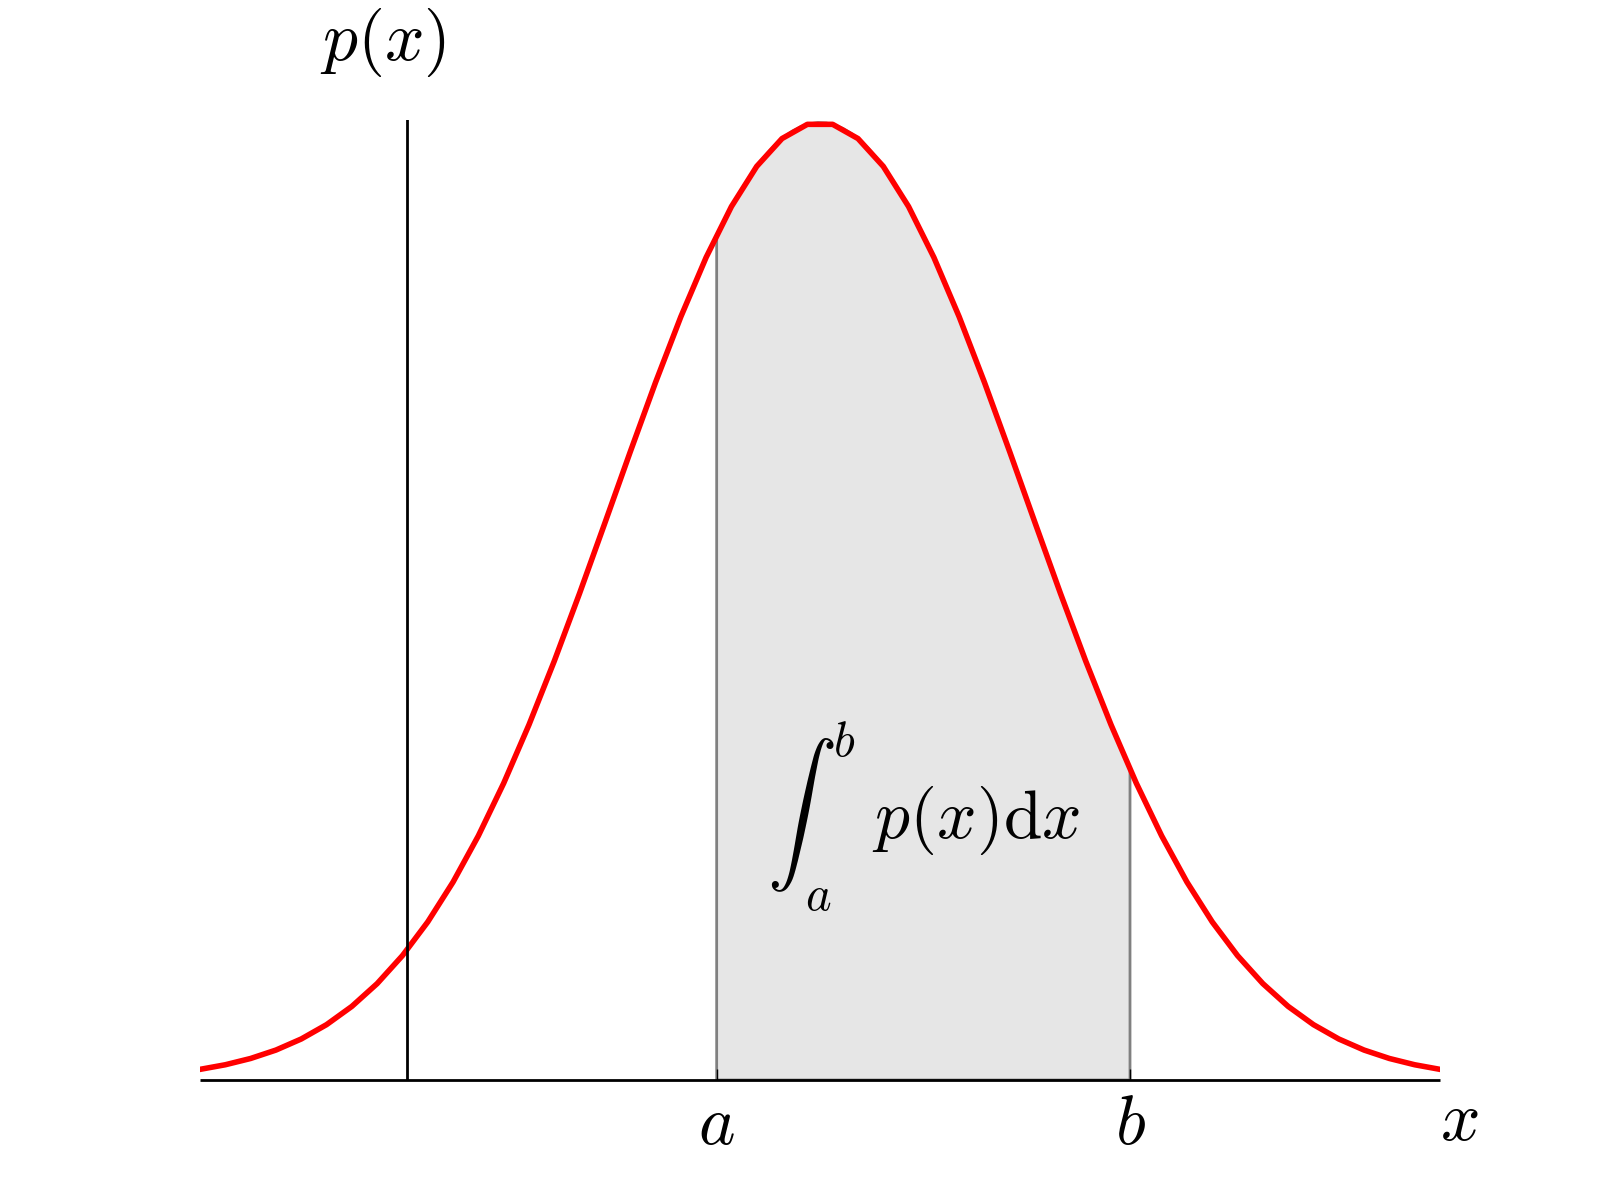
\includegraphics[width=0.5\textwidth]{../Images/PDF.png}\\
  \caption{Probability Density Function (PDF) of a value x. The integral over the PDF between a and b gives the likelihood of finding the value of x in that range.}\label{fig:PDF}
\end{figure}

\subsubsection{Cumulative Density Function (CDF)}\index{general}{cumulative density function}

The probability to find a value between $a$ and $b$ is given by the integral over the PDF in that range (see Fig. \ref{fig:PDF}), and the \emph{Cumulative Density Function} tells you for each value which percentage of the data has a lower value (Figure \ref{fig:CDF}). Together, this gives us

\begin{equation}
   \mathbb{P}(a \leq X \leq b) = \int\limits_a^b {PDF(x)dx} = CDF(b) - CDF(a)
\end{equation}


\begin{figure}[ht]
  \centering
  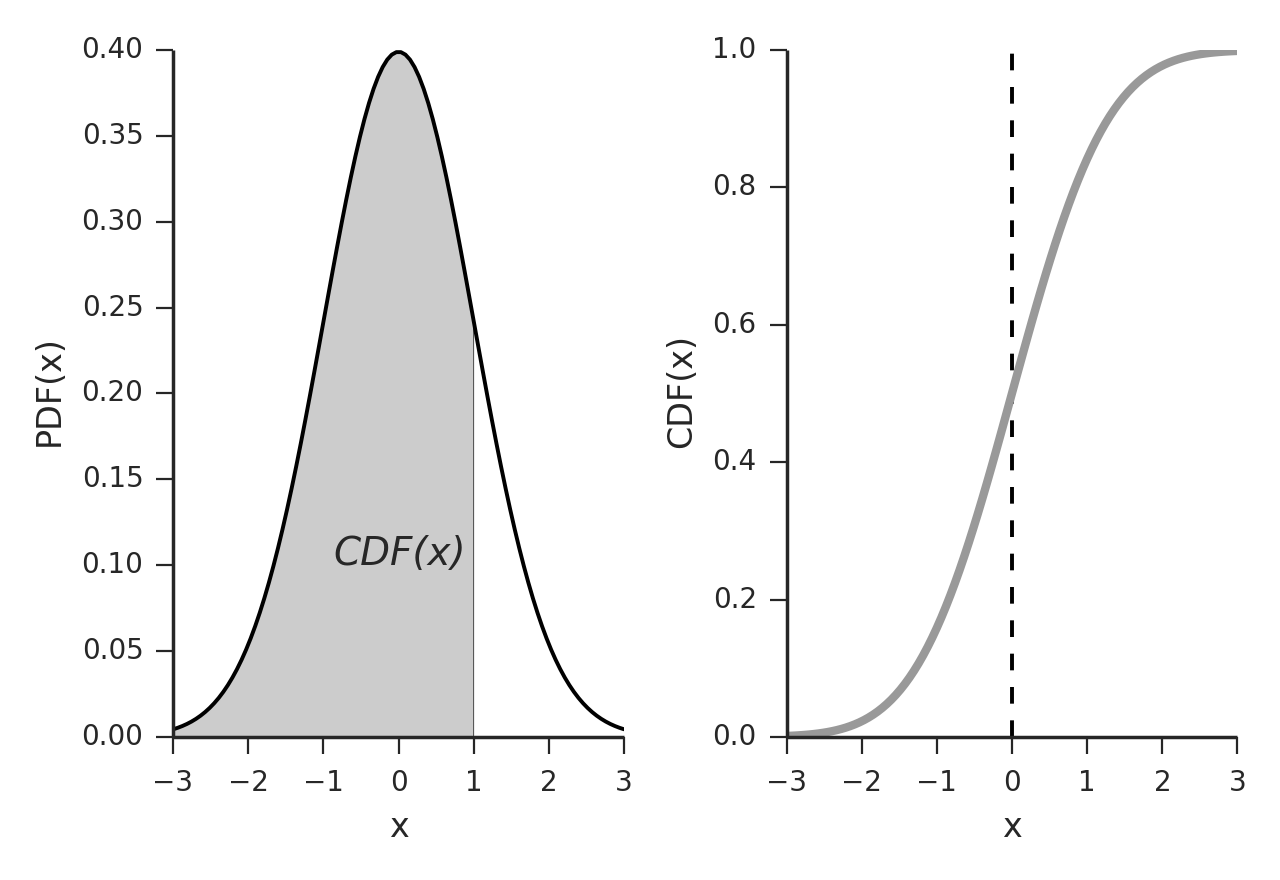
\includegraphics[width=0.5\textwidth]{../Images/PDF_CDF.png}\\
  \caption{\emph{Probability density function} (left) and \emph{Cumulative density function} (right) of a normal distribution.}\label{fig:CDF}
\end{figure}

\subsubsection{Other important presentations of Probability Densities}\index{general}{cumulative density function}

Figure \ref{fig:DistributionUtilities} shows a number of functions that are equivalent to the PDF, but each represent a different aspect of the probability distribution.

\textbf{Note: }It is very important that you understand this figure!

\begin{itemize}
  \item \emph{Probability density function (PDF)}: note that to obtain the probability for the variable appearing in a certain interval, you have to \emph{integrate} the PDF over that range.
  \item \emph{Cumulative distribution function (CDF)}: gives the probability of obtaining a value smaller than the given value.
  \item \emph{Survival function (SF)}: 1-CDF: gives the probability of obtaining a value larger than the given value. It can also be interpreted as the proportion of data "surviving" above a certain value.
  \item \emph{Percentile point function (PPF)}: the inverse of the CDF. Answers the question "Given a certain probability, what is the corresponding value for the CDF?"
  \item \emph{Inverse survival function (ISF)}: the name says it all.
\end{itemize}

\begin{figure}[h]
  \centering
  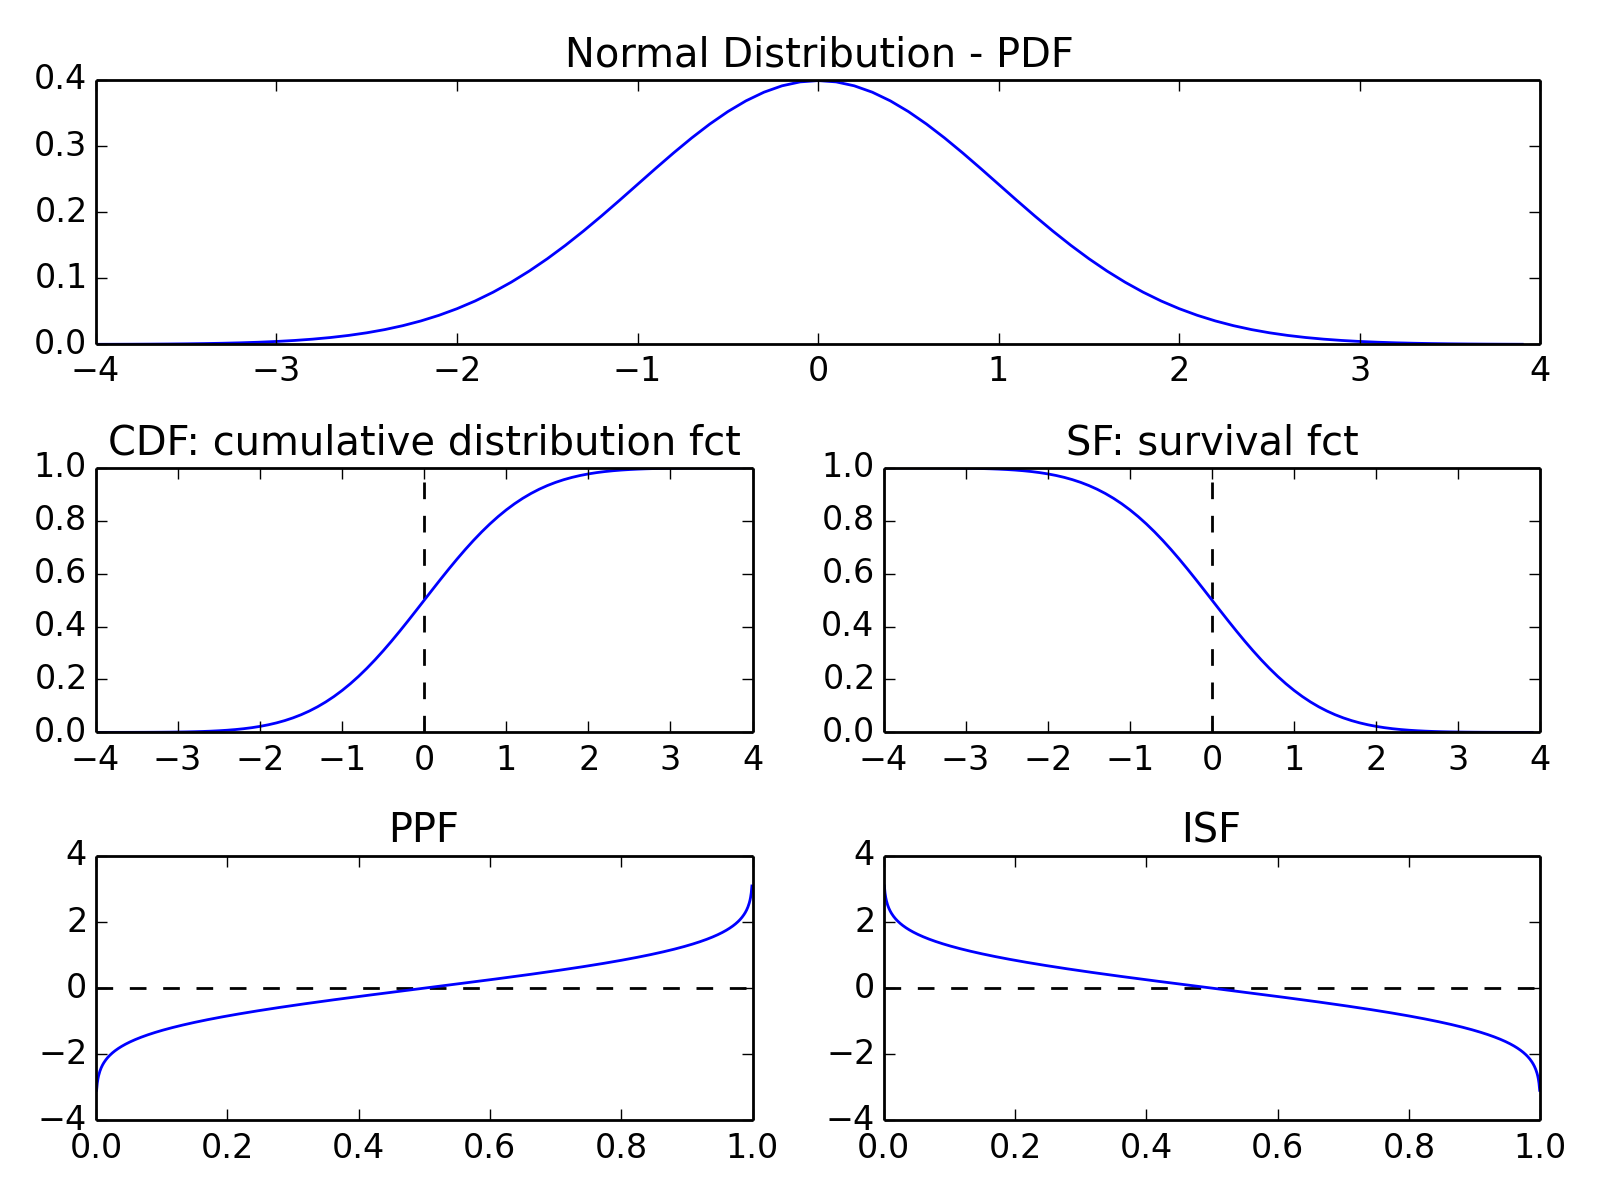
\includegraphics[width=0.95\textwidth]{../Images/DistributionFunctions.png}\\
  \caption{Utility functions for continuous distributions, here for the normal distribution.}\label{fig:DistributionUtilities}
\end{figure}

\subsection{Distribution Center}

When we have a datasample from a distribution, we can characterize the center of the distribution with different parameters:

\subsubsection{Mean} \index{general}{mean}
By default, when we talk about the \emph{mean value} we mean the \emph{arithmetic mean} $\bar{x}$:

\begin{equation}
  \bar{x} = \frac{{\sum\limits_{i = 1}^n {{x_i}} }}{n}
\end{equation}

\subsubsection{Median} \index{general}{median}
The \emph{median} is that value that comes half-way when the data are ranked in order.
In contrast to the mean, it is not affected by outlying data points.

\subsubsection{Mode} \index{general}{mode}
The \emph{mode} value is the most frequently occurring value in a distribution.

\subsubsection{Geometric Mean}\index{general}{geometric mean}
In some situations the \emph{geometric mean} can be useful to describe the location of a distribution. It is usually close to the median, and can be calculated via the arithmetic mean of the log of the values.

\subsection{Quantifying Variability}\label{sec:centiles}

\subsubsection{Range}\index{general}{range}
This one is fairly easy: it is the difference between the highest and the lowest data value.
The only thing that you have to watch out for: after you have acquired your data, you have to check for \emph{outliers}, i.e. data points with a value much higher or lower than the rest of the data. Often, such points are caused by errors in the selection of the sample or in the measurement procedure. There are a number of tests to check for outliers. One of them is to check for data which lie more than 1.5*\emph{inter-quartile-range} (IQR) above or below the first/third quartile (see below).


\subsubsection{Percentiles}\index{general}{centiles}\index{general}{percentiles}

\emph{Centiles}, also called \emph{percentile}, give the value below which a given percentage of the values occur. It corresponds to a value with a specified cumulative frequency. While you won't often hear the expression \emph{centiles}, you will frequently encounter specific centiles:

\begin{itemize}
  \item When you look for the data range which includes 95\% of the data, you have to find the $2.5^{th}$ and the $97.5^{th}$ percentile of your sample distribution.
  \item The 50th percentile is the \emph{median}.
  \item Also important are the \emph{quartiles}, i.e. the 25th and the 75th percentile. The difference between them is sometimes referred to as \emph{inter-quartile range (IQR)}\index{general}{IQR}.
\end{itemize}

Median, upper and lower quartile are used for the data display in box plots (Fig.\ref{fig:Boxplot}).

\subsubsection{Standard Deviation and Variance}
The \emph{variance} (SD) of a distribution is defined as

\begin{equation}\label{eq_variance} \index{general}{variance}
  var = \frac{{\sum\limits_{i = 1}^n {({x_i-\bar{x}})^2} }}{n-1}
\end{equation}

Note that we divide by \emph{n-1} rather than the more obvious n: dividing by $n$ gives the variance of the observations around the sample mean, but we virtually always consider our data as a sample from some larger population and wish to use the sample data to estimate the variability in the population. Dividing by $n-1$ gives us a better estimate of the population variance.

Figure \ref{fig:mean_std} indicates why the sample standard deviation underestimates the standard deviation of the underlying distribution.

\begin{figure}[ht]
  \centering
  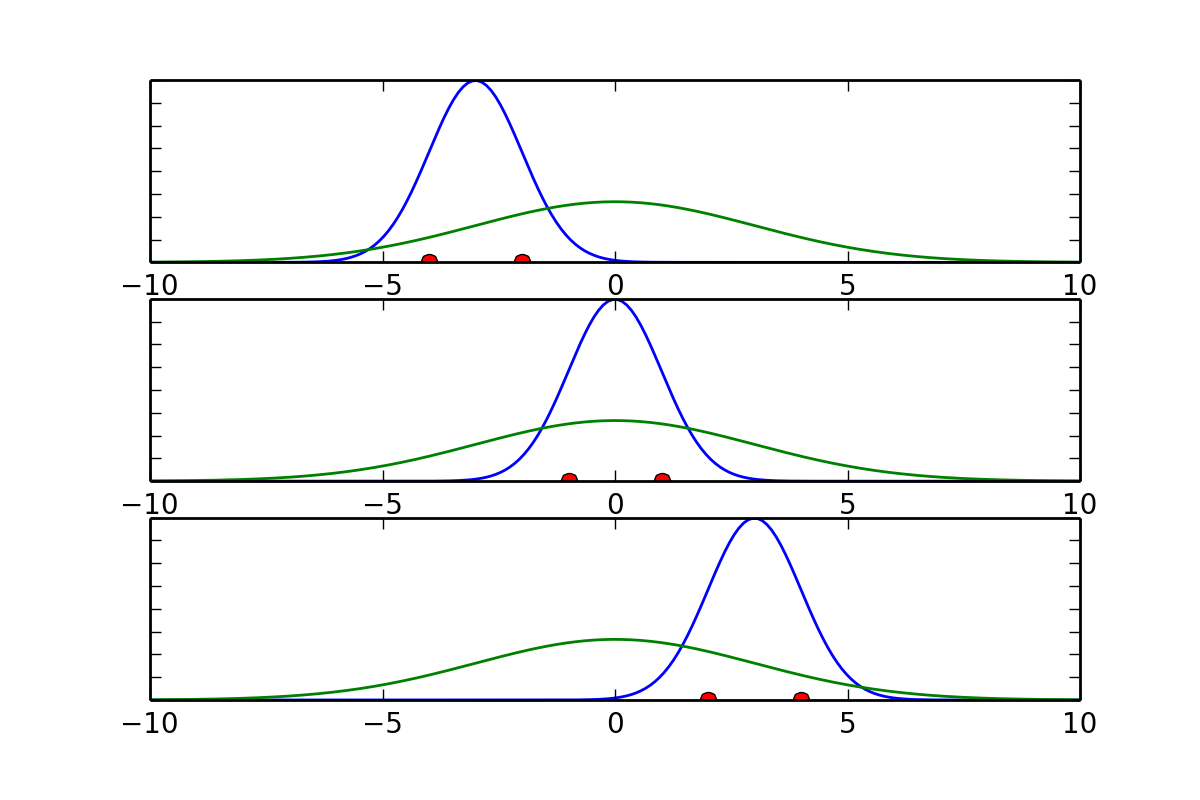
\includegraphics[width=0.5\textwidth]{../Images/mean_std.png}\\
  \caption{Gaussian distributions fitted to selections of data from the underlying distribution: While the average mean of a number of samples converges to the real mean, the sample standard deviation underestimates the standard deviation from the distribution.}\label{fig:mean_std}
\end{figure}

The \emph{standard deviation} \index{general}{standard deviation} is simply given by the square root of the variance:

\begin{equation}
  s = \sqrt{var}
\end{equation}

In statistics it is often common to denote the population standard deviation with $\sigma$, and the sample standard deviation with $s$.

Watch out: in Python, by default the variance is calculated for "n". You have to set "ddof=1" to obtain the variance for "n-1":

\begin{lstlisting}
    In[19]: data = arange(7,14)

    In[20]: std(data, ddof=0)
    Out[20]: 2.0

    In[21]: std(data, ddof=1)
    Out[21]: 2.1602468994692865
\end{lstlisting}

\subsubsection{Standard Error} \index{general}{standard error}
While the standard deviation is a good measure for the distribution of your values, often you are more interested in the distribution of the mean value. For example, when you measure the response to a new medication, you might be interested in how well you can characterize this response, i.e. is how well you know the mean value. This measure is called the \emph{standard error of the mean}, or sometimes just the \emph{standard error}. In a single sample from a population with a standard deviation of $\sigma$ the variance of the sampling distribution of the mean is $\sigma^2/n$, and so the standard error of the mean is $\sigma/\sqrt{n}$.

For the \emph{sample standard error of the mean}, which is the one you will be working with most of the time, we have

\begin{equation}
  SE = \frac{s}{\sqrt{n}} = \sqrt{\frac{{\sum\limits_{i = 1}^n {({x_i-\bar{x}})^2} }}{n-1}} \cdot \frac{1}{\sqrt{n}}
\end{equation}

\subsubsection{Confidence Intervals}\index{general}{confidence interval}
The most informative parameter that you can give for a statistical variable is arguably its \emph{confidence interval}. The confidence interval reports the range that contains the true value for your parameter with a likelihood of $\alpha$\%.

Most of the time you want to determine the confidence interval for normally distributed data, which is given by

\begin{equation}
  ci = mean \pm std * t_{df,\alpha}
\end{equation}\label{eq:ci}

where $std$ is the sample standard deviation, and $t_{df,\alpha}$ the $t$ statistic (which will be covered later in this chapter) for $df$ degrees of freedom. For the 95\% two-sided confidence intervals, for example, you have to set $\alpha=0.025$ and $\alpha=0.975$ .

\textbf{Note:} If you want to know the confidence interval for the mean value, you have to replace the \emph{standard deviation} by the \emph{standard error}! In Python, the 95\% confidence interval for the mean can be obtained with a one-liner:

\begin{lstlisting}
    alpha = 0.95
    df = len(data)-1
    ci = stats.t.interval(alpha, df, loc=mean(data), scale=stats.sem(data))
\end{lstlisting}

\subsection{Parameters Describing the Form of a Distribution}

\subsubsection{Location}

A \emph{location parameter} $x_0$  determines the "location" or shift of a distribution.

\begin{equation*}
  f_{x0}(x)=f(x-x_0)
\end{equation*}

Examples of location parameters include the mean, the median, and the mode.

\subsubsection{Scale}

The \emph{scale parameter} describes the width of a probability distribution.  If s is large, then the distribution will be more spread out; if s is small then it will be more concentrated. If the probability density exists for all values of $s$, then the density (as a function of the scale parameter only) satisfies

\begin{equation*}
   f_s(x) = f(x/s)/s,
\end{equation*}

where f is the density of a standardized version of the density.

\subsubsection{Shape Parameters}\index{general}{shape parameters}

A shape parameter is any parameter of a probability distribution that is neither a location parameter nor a scale parameter. If \emph{location }and \emph{shape} already completely determine the distribution (as is the case for e.g. the normal distribution or the exponential distribution, etc.), then these distributions don't have any \emph{shape parameter}. It follows that the \emph{skewness }and \emph{kurtosis} of these distribution are constants.


\subsubsection{Skewness}\index{general}{skewness}

Distributions are \emph{skewed} if they depart from symmetry. For example, if you have a measurement that cannot be negative, which is usually the case, then we can infer that the data have a skewed distribution if the standard deviation is more than half the mean. Such an asymmetry is referred to as \emph{positive skewness}. The opposite, negative skewness, is rare.


\begin{figure}
\centering
\begin{subfigure}{.5\textwidth}
  \centering
  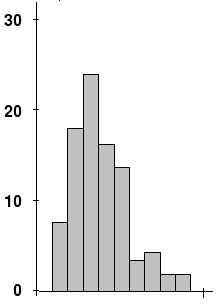
\includegraphics[width=0.4\textwidth]{../Images/SkewedDistribution.png}\\
  \caption{Example of experimental data with non-zero (positive) skewness.}
  \label{fig:skewness}
  \end{subfigure}%
\begin{subfigure}{.5\textwidth}
  \centering
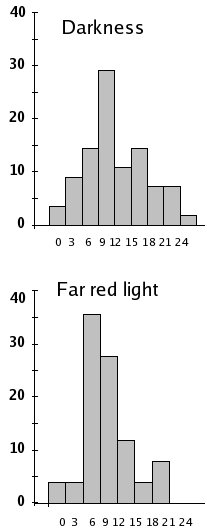
\includegraphics[width=0.3\textwidth]{../Images/KurtosisChanges.png}\\
  \caption{The "Darkness" data is platykurtic (−0.194), while "Far Red Light" shows leptokurtosis (0.055).}
  \label{fig:kurtosis}
  \end{subfigure}
\caption{Skew and Kurtosis of distributions (from Wikipedia).}
\label{fig:skewkurtosis}
\end{figure}


\subsubsection{Kurtosis}\index{general}{kurtosis}

Kurtosis is any measure of the "peakedness" of the probability distribution. Distributions with negative or positive excess kurtosis are called platykurtic distributions or leptokurtic distributions respectively.

%(Lecture 5)

\section{Distribution Functions}

The variable for a standardized distribution function is often called \emph{statistic}\index{general}{statistic}. So you often find expressions like "the z-statistic" (for the normal distribution function), the "t-statistic" (for the t-distribution) or the "F-statistic" (for the F-distribution).

\subsection{Normal Distribution} \label{sec:normalDistribution}\index{general}{distributions!normal}

The \emph{Normal distribution} or \emph{Gaussian distribution} is by far the most important of all the distribution functions. This is due to the fact that the mean values of \emph{all} distribution functions approximate a normal distribution for large enough sample numbers.
Mathematically, the normal distribution is characterized by a mean value $\mu$, and a standard deviation $\sigma$:

\begin{equation}\label{eq_normal}
     f_{\mu,\sigma} (x) = \frac{1}{\sigma \sqrt{2 \pi}} e^{-( x - \mu )^2 /2 \sigma^2}
\end{equation}
where $ - \infty < x < \infty $, and $f_{\mu,\sigma}$ is the \emph{probability density function (PDF)} \index{general}{probability density function}.

\begin{figure}
  \centering
  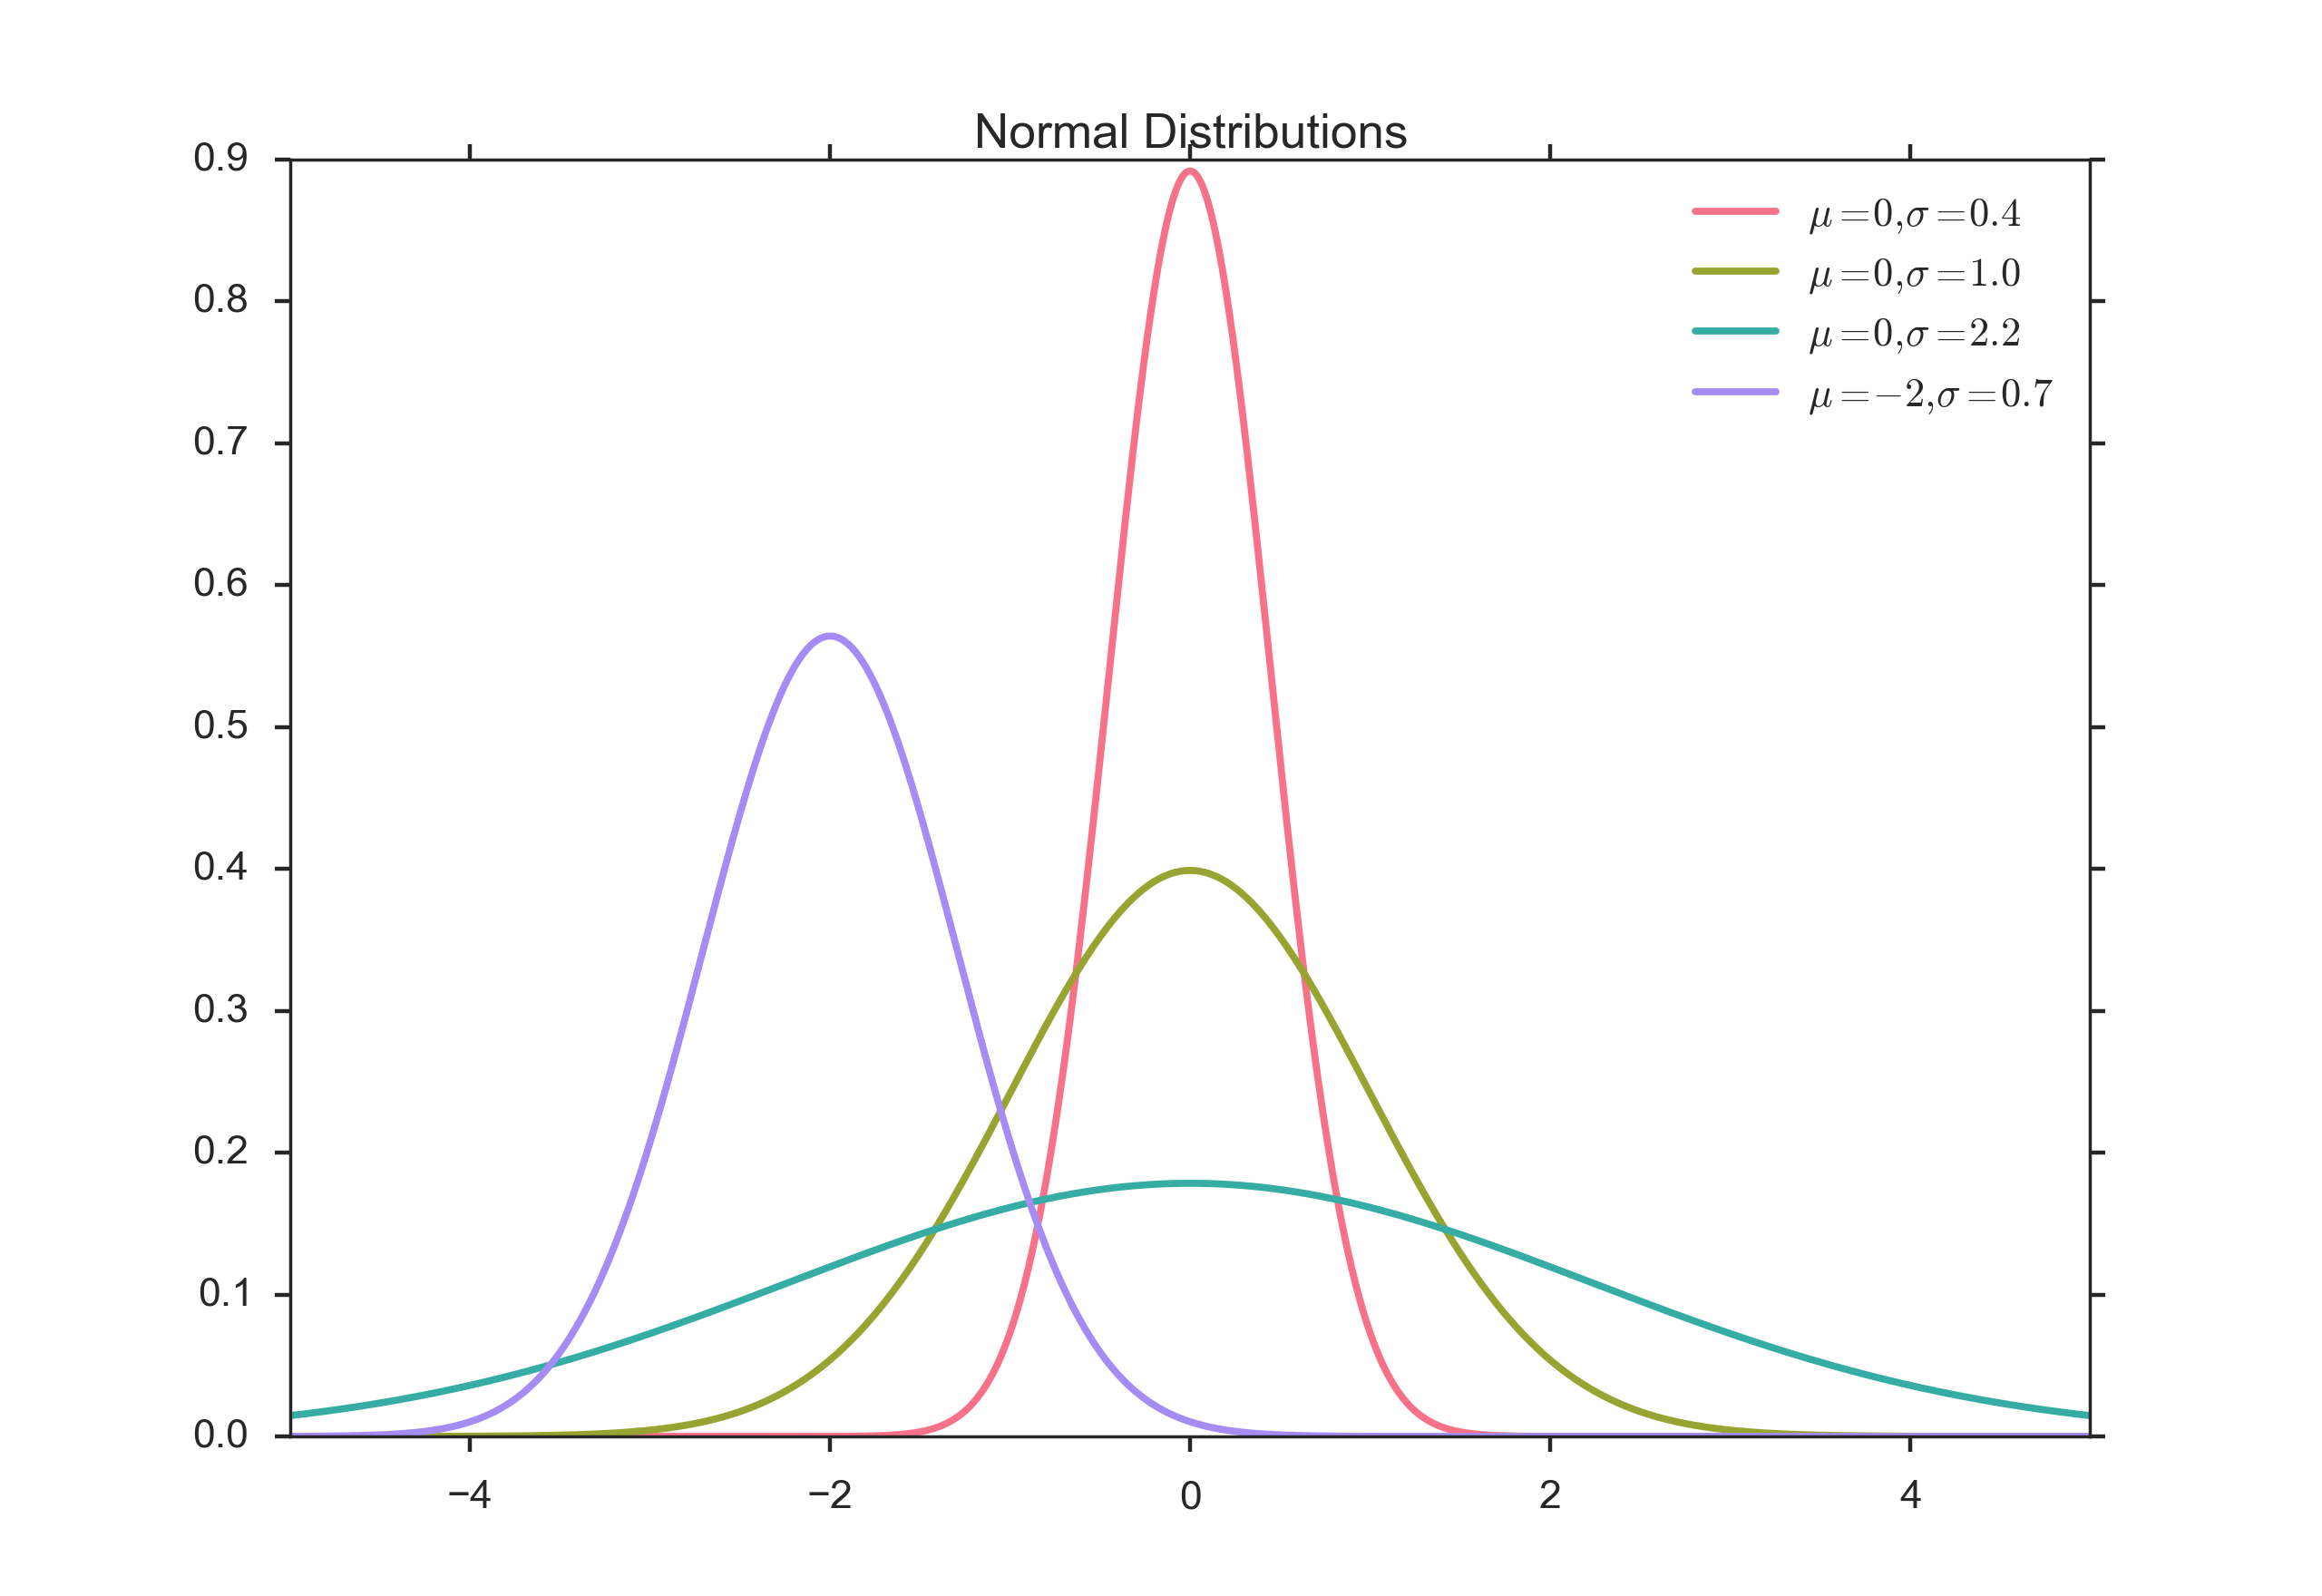
\includegraphics[width=0.75\textwidth]{../Images/Normal_Distribution_PDF.png}\\
  \caption{Normal Distribution}\label{fig:normal}
\end{figure}

For smaller sample numbers, the sample distribution can show quite a bit of variability. For example, look at 25 distributions generated by sampling 100 numbers from a normal distribution (Fig. \ref{fig:MultipleNormal})

\begin{figure}[h]
  \centering
  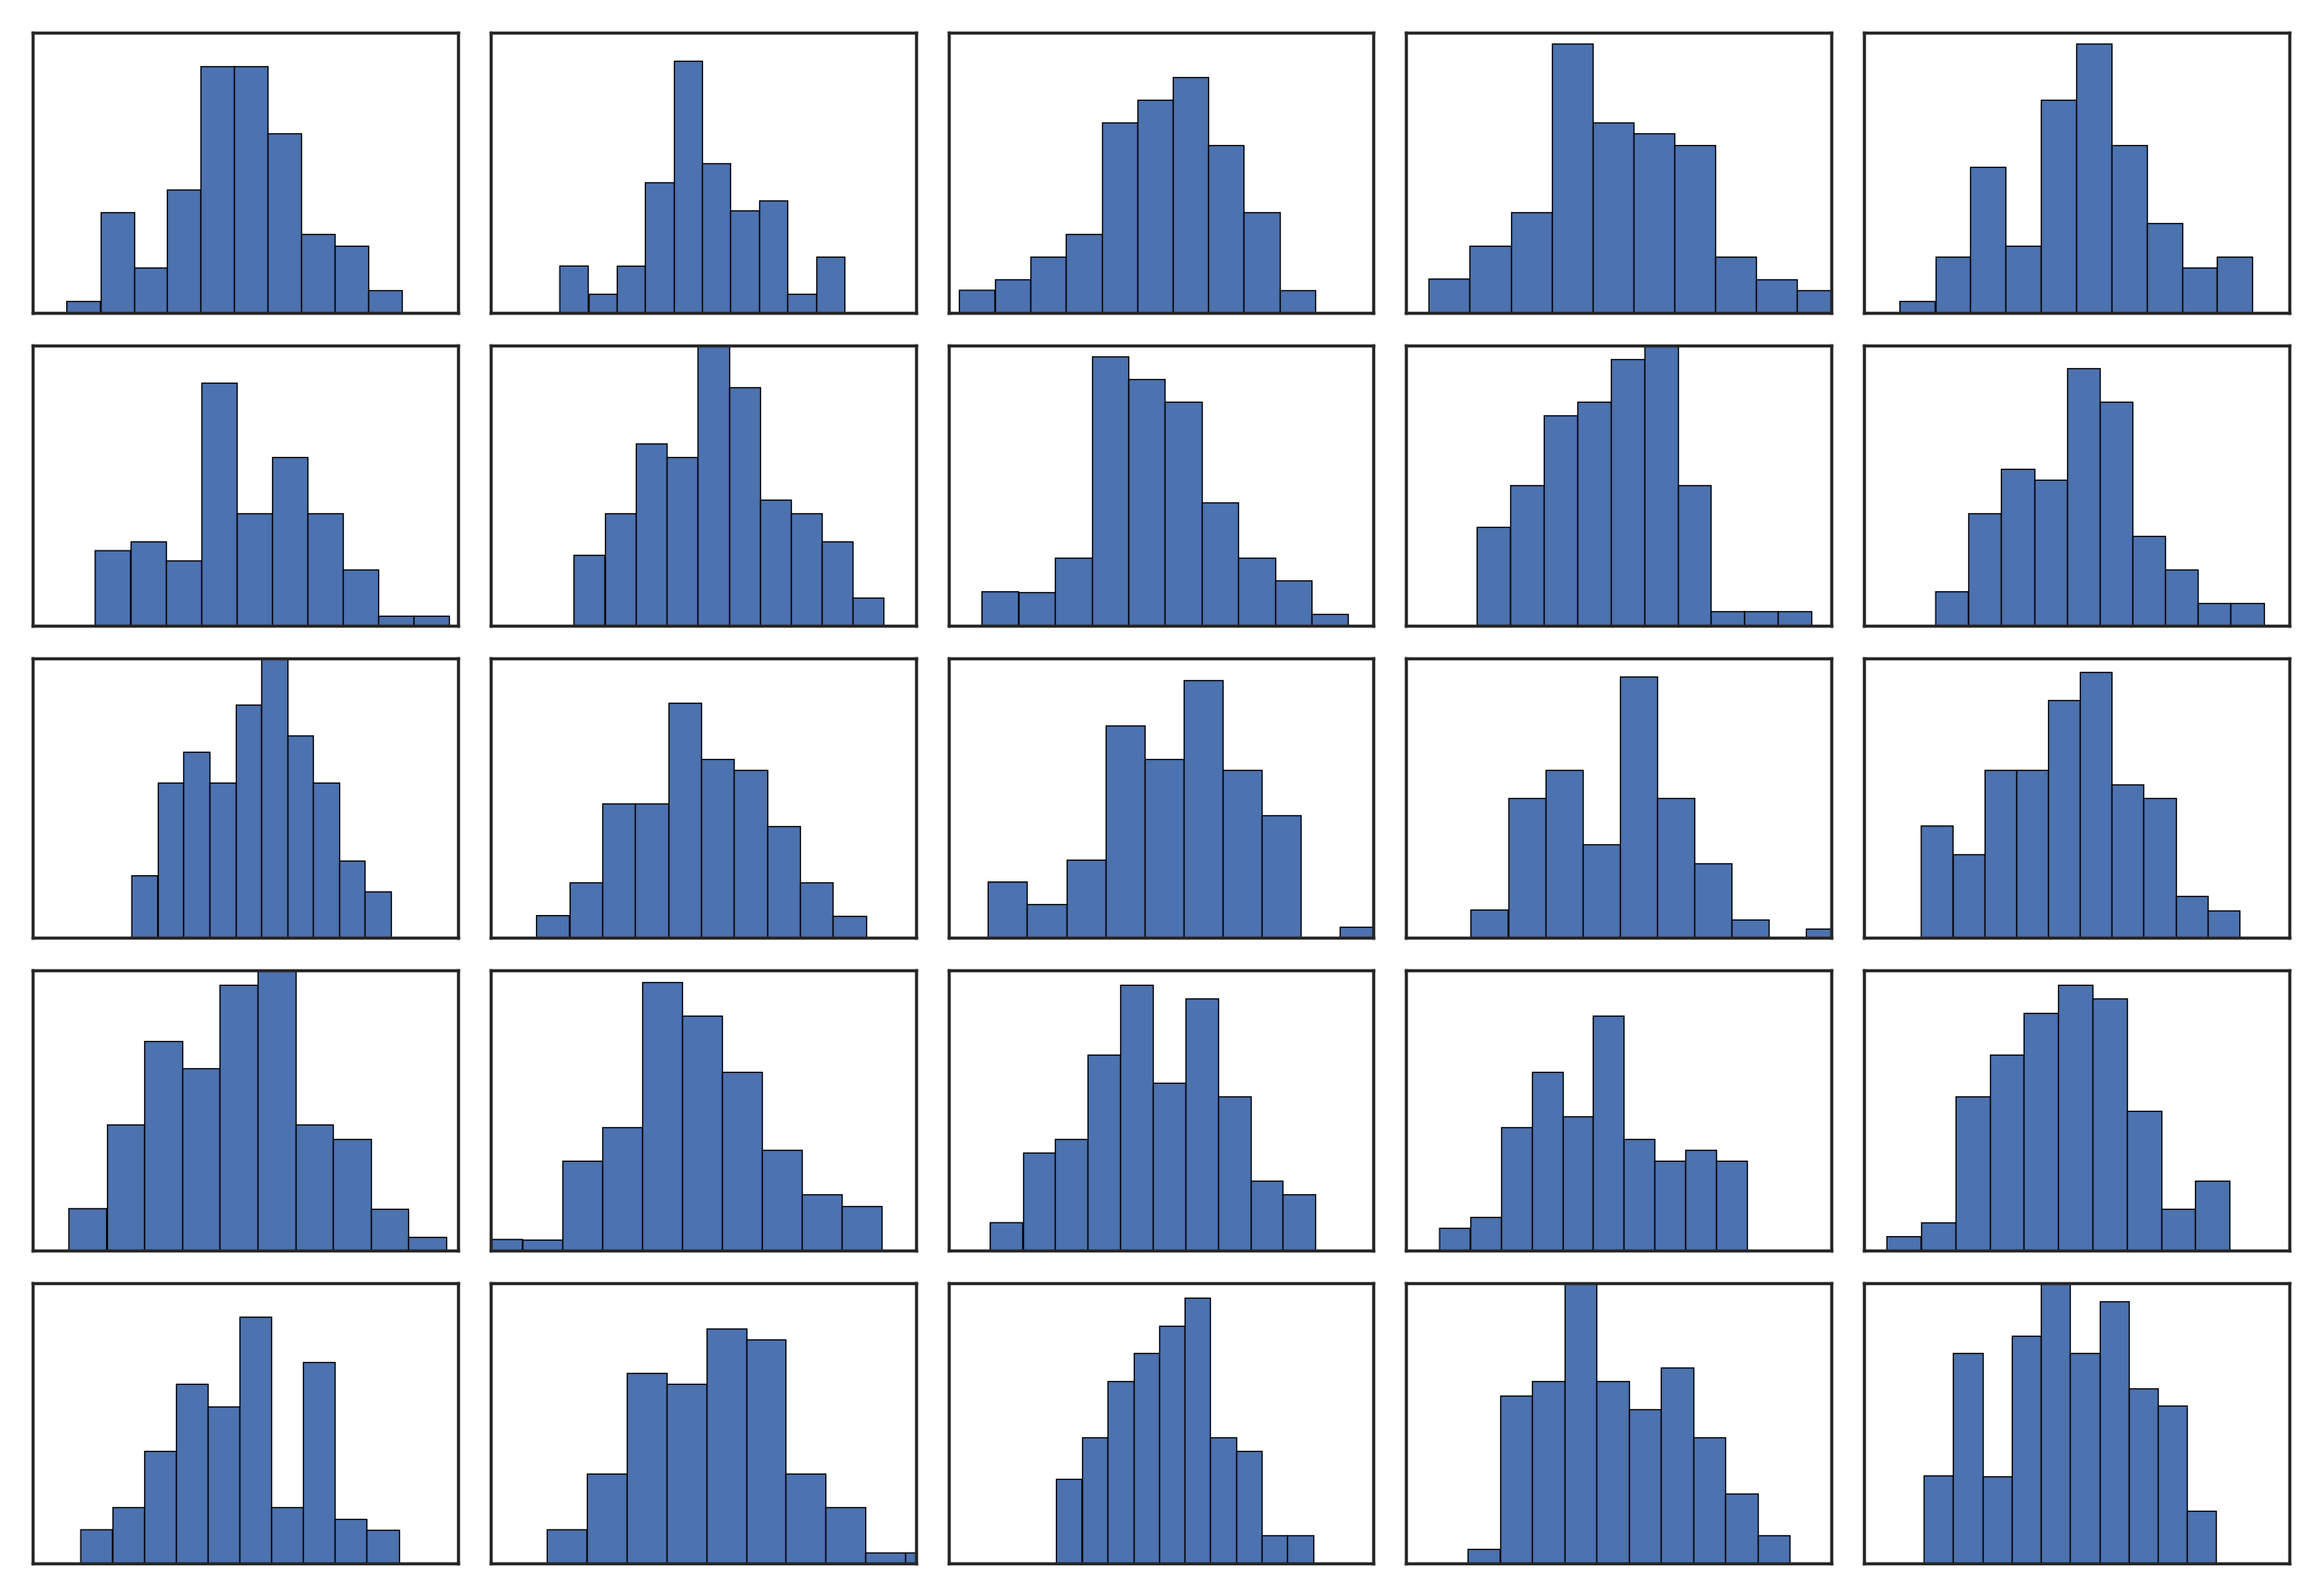
\includegraphics[width=0.75\textwidth]{../Images/Normal_MultHist.png}\\
  \caption{25 randomly generated normal distributions of 100 points.}\label{fig:MultipleNormal}
\end{figure}

Some examples of applications are:

\begin{itemize}
    \item{}If the average man is 175 cm tall with a standard deviation of 6 cm, what is the probability that a man found at random will be 183 cm tall?
    \item{}If the average man is 175 cm tall with a standard deviation of 6 cm and the average woman is 168 cm tall with a standard deviation of 3 cm, what is the probability that the average man from a given sample will be shorter than the average woman from a given sample?
    \item{}If cans are assumed to have a standard deviation of 4 grams, what does the average weight need to be in order to ensure that the 99\% of all cans have a weight of at least 250 grams?
\end{itemize}

The normal distribution with parameters $\mu$ and $\sigma$ is denoted as {$N(\mu,\sigma)$}. If the \emph{random variate (rv)} {\itshape X} is normally distributed with expectation $\mu$ and standard deviation $\sigma$, one denotes: {$\,X \sim N(\mu,\sigma)$} or $\,X \in N(\mu,\sigma)$.

\begin{figure}
  \centering
  % Requires \usepackage{graphicx}
  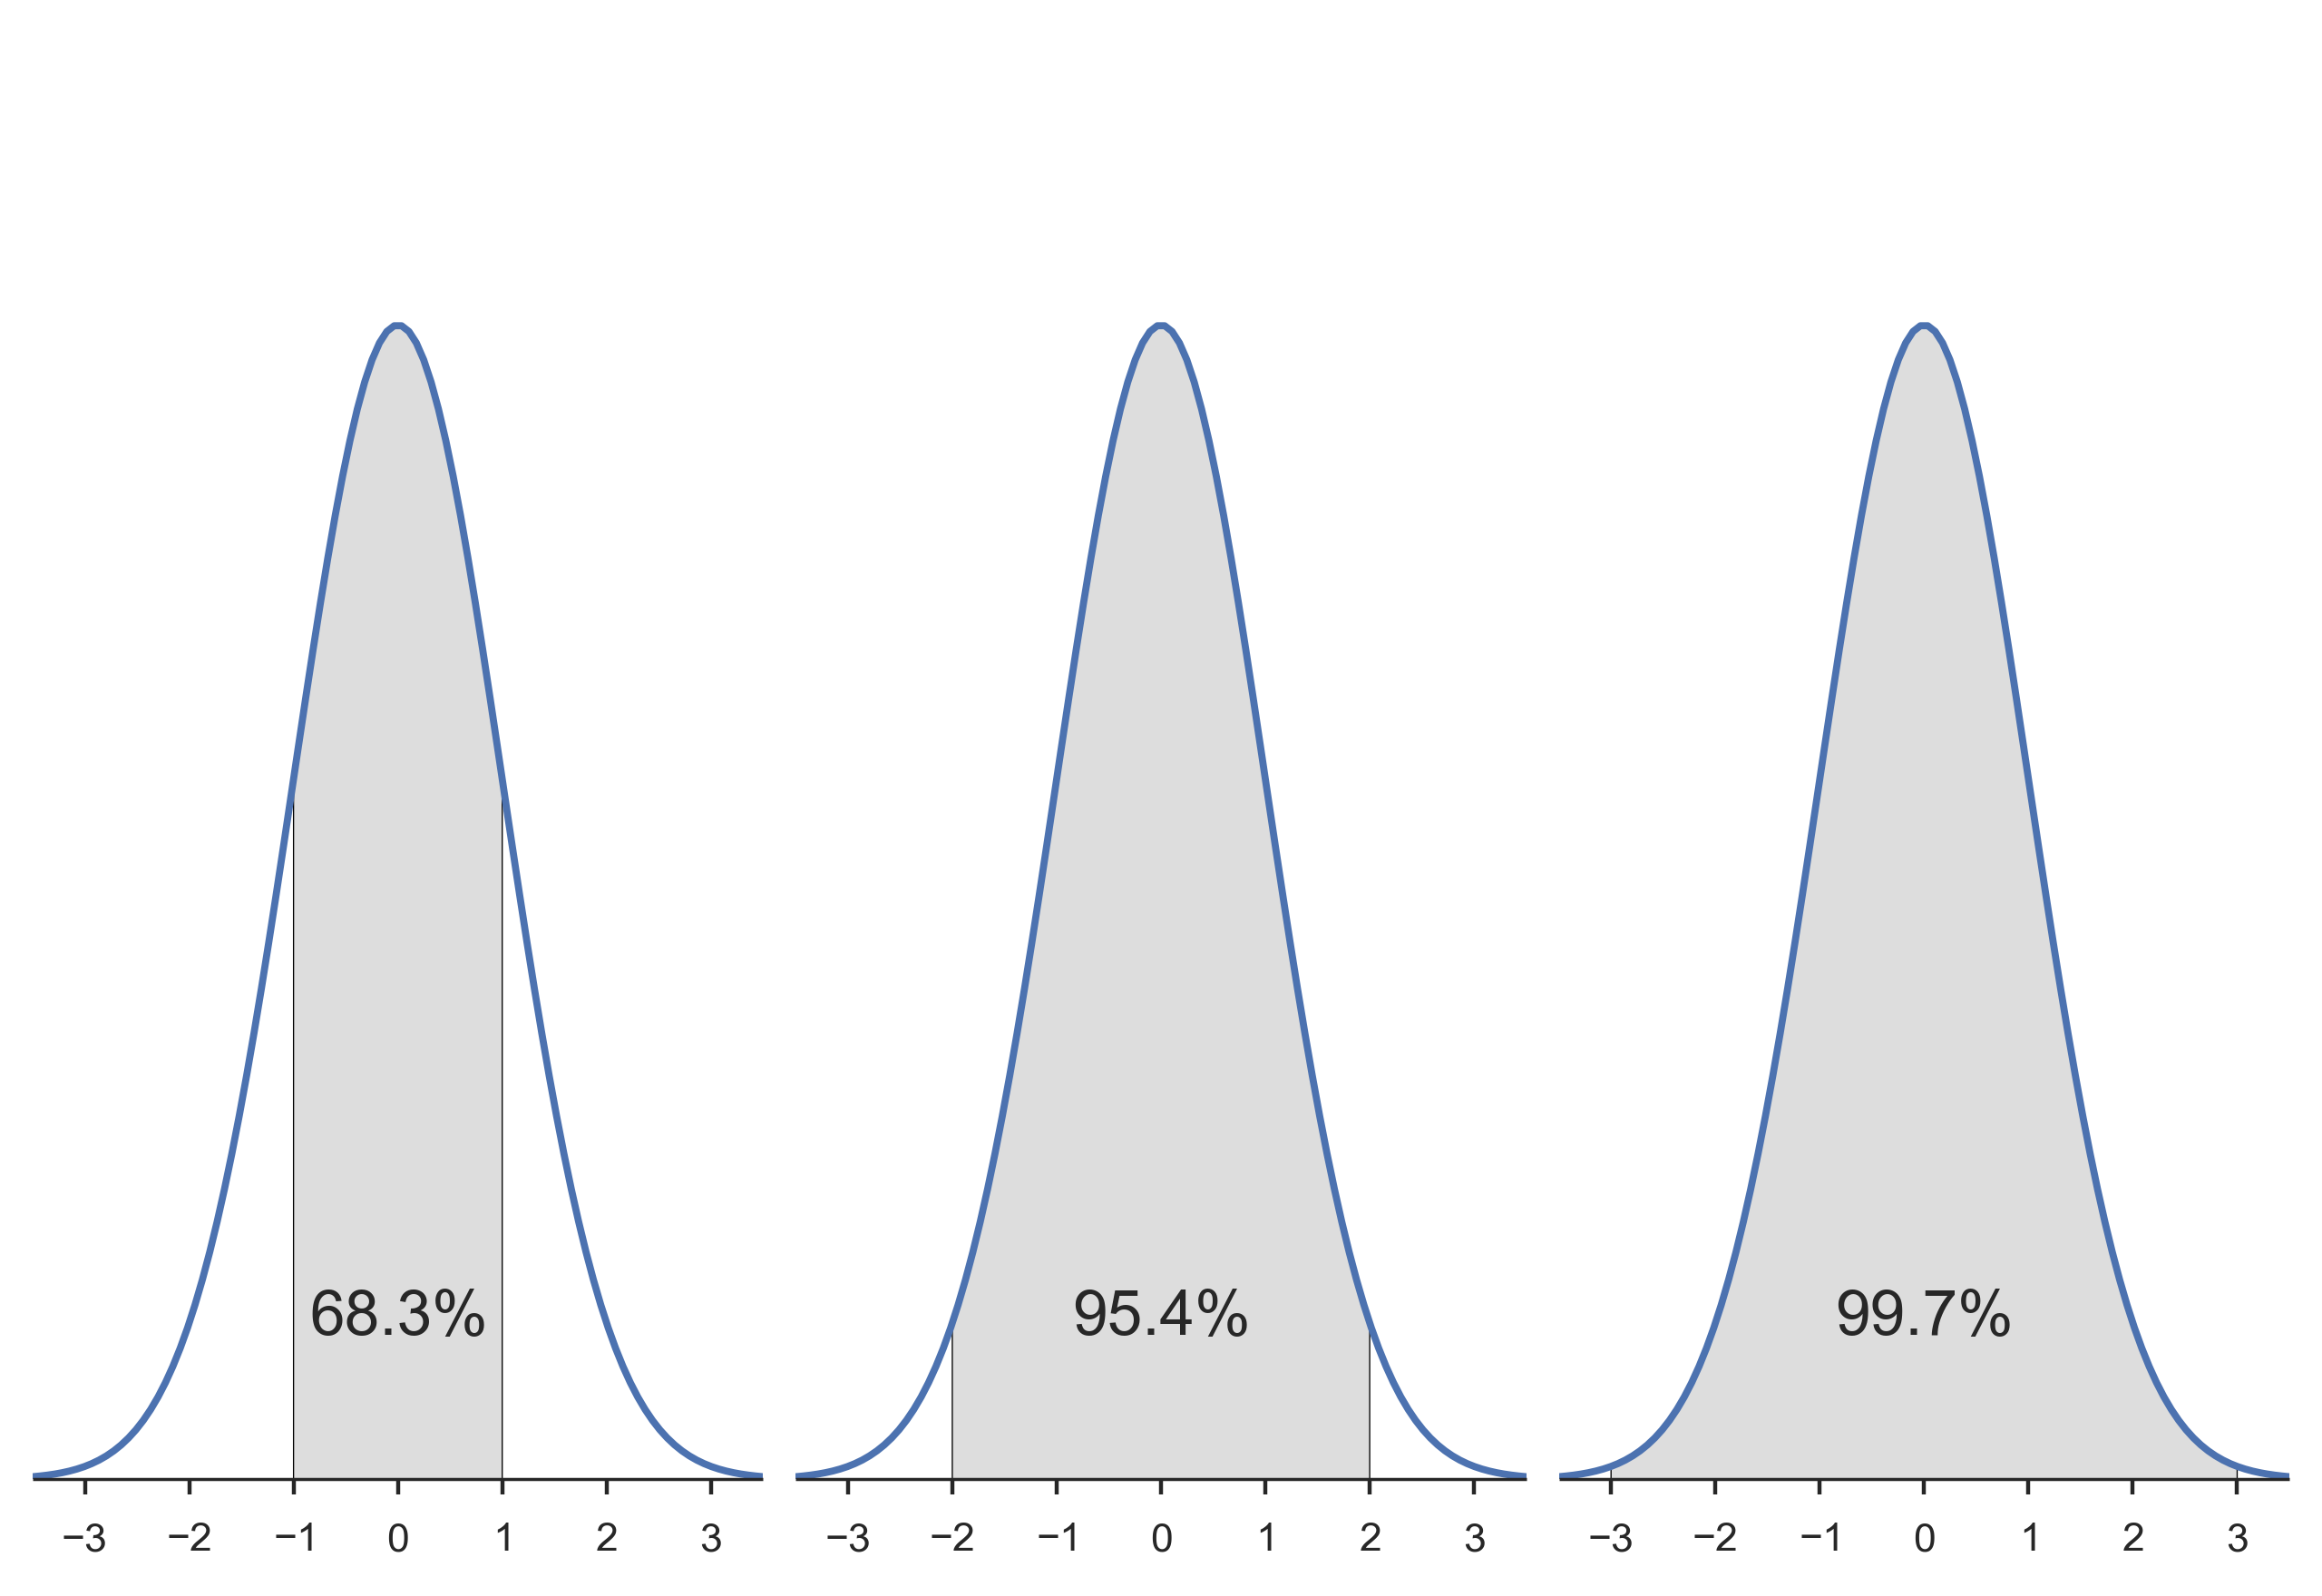
\includegraphics[width=0.8\textwidth]{../Images/area_SDs.png}\\
  \caption{Area under +/1 1, 2, and 3 standard deviations of a normal distribution.}\label{fig:area_SDs}
\end{figure}


\begin{table}
  \centering
  \begin{tabular}{c c c}
    \hline
     & \multicolumn{2}{ c } {Probability of being} \\
    Range & within range & outside range \\
    \hline
    % after \\: \hline or \cline{col1-col2} \cline{col3-col4} ...
    mean $\pm$ 1SD & 0.683 & .317 \\
    mean $\pm$ 2SD & 0.954 & 0.046 \\
    mean $\pm$ 3SD & 0.9973 & 0.0027 \\
    \hline
  \end{tabular}
  \caption{Tails of a normal distribution.}
\end{table}



\vspace{5 mm}
\fbox{%
\begin{minipage}{15 cm}

\textbf{Note:}
In Python, the most elegant way of working with distribution function is a two-step procedure:
\begin{itemize}
  \item In the first step, you create your distribution (e.g. \textsf{nd = stats.norm()}). Note that is a \emph{distribution} (in Python parlance a "frozen distribution"), not a function yet!
  \item In the second step, you decide which function you want to use from this distribution, and calculate the function value for the desired x-input (e.g. \textsf{y = nd.cdf(x)})
\end{itemize}

\end{minipage}}
\vspace{10 mm}

\PyImg "distributionNormal.py" (p \pageref{py:distributionNormal}) shows simple manipulations of normal distribution functions.
\index{python}{distributionNormal}

\begin{lstlisting}
  In [33]:  from scipy import stats
  In [34]:  mu = -2
  In [35]:  sigma = sqrt(0.5)
  In [36]:  myDistribution = stats.norm(mu, sigma)
  In [37]:  significanceLevel = 0.05
  In [38]:  myDistribution.ppf([significanceLevel/2, 1-significanceLevel/2])
  Out[38]:  array([-3.38590382, -0.61409618]
\end{lstlisting}
\emph{Example of how to calculate the interval of the PDF containing 95\% of the data, for the green curve in Figure \ref{fig:normal}}

\subsection{Central Limit Theorem}\index{general}{central limit theorem}
The central limit theorem states that for identically distributed independent random variables (also referred to as \emph{random variates})\index{general}{variate}, the mean of a sufficiently large number of these variables will be approximately normally distributed.
\ref{fig:CentralLimitTheorem} shows that averaging over 10 uniformly distributed data already produces a smooth, almost Gaussian distribution.

\begin{figure}
  \centering
  % Requires \usepackage{graphicx}
  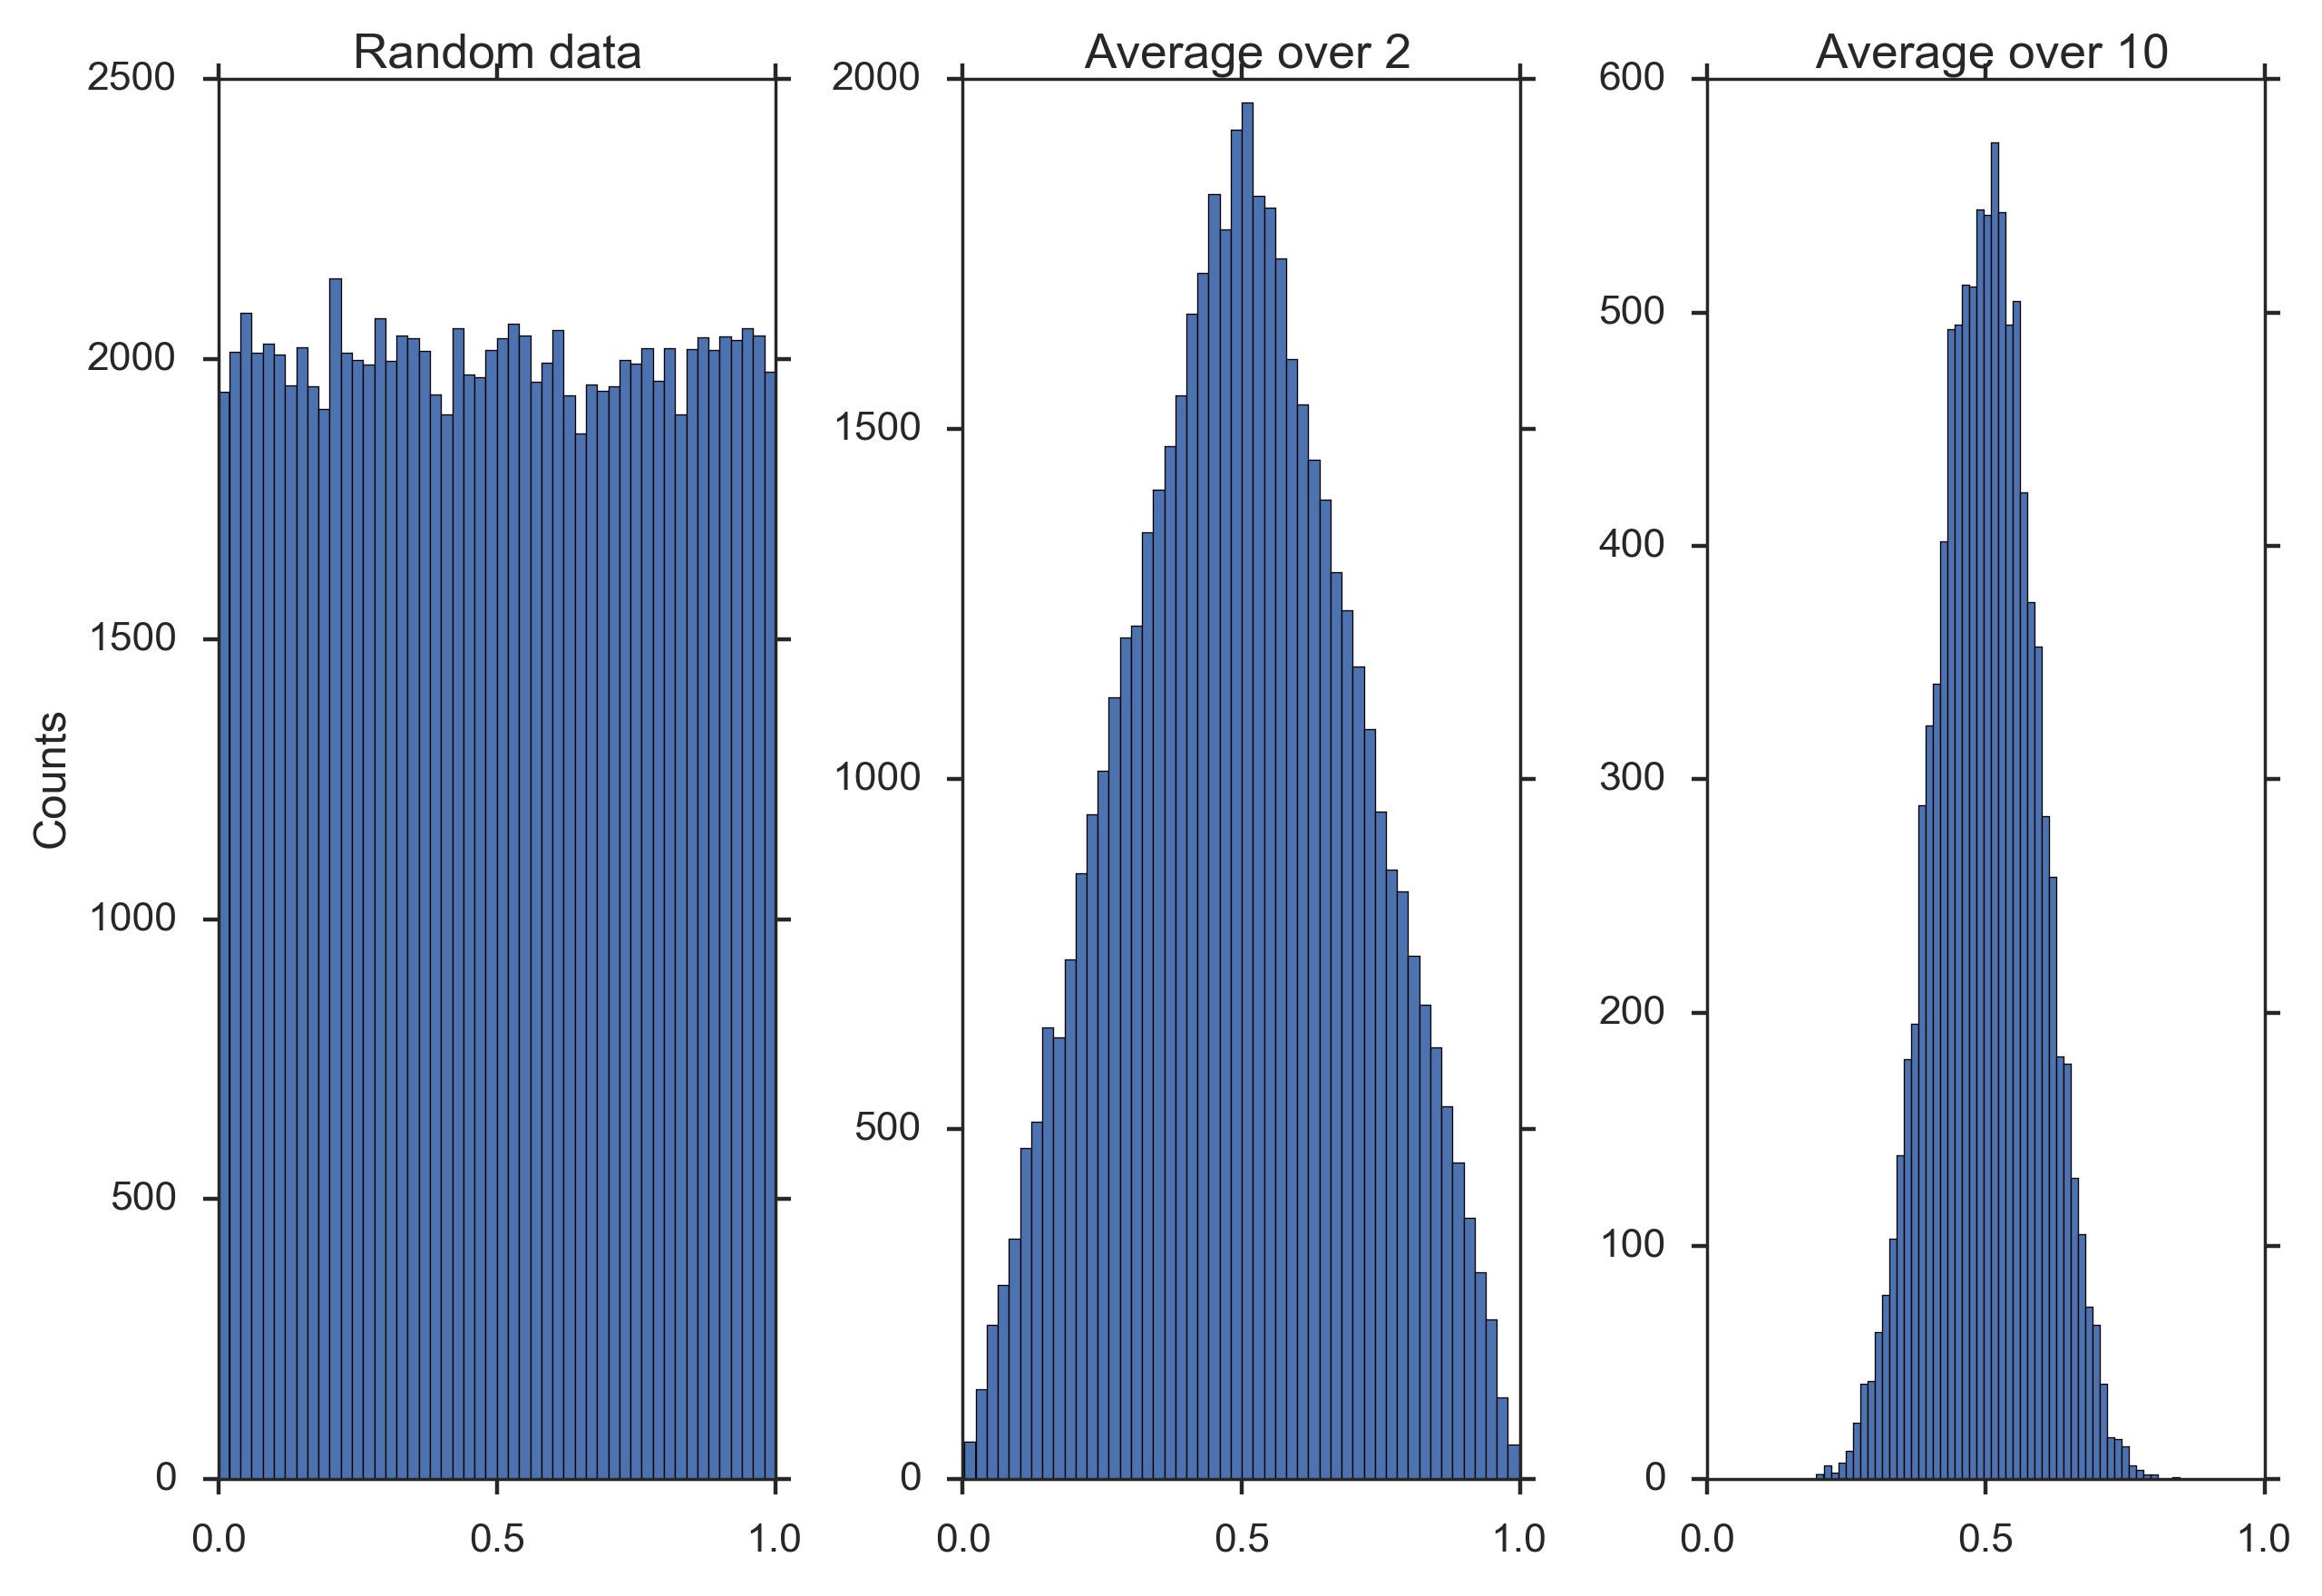
\includegraphics[width=0.7\textwidth]{../Images/CentralLimitTheorem.png}\\
  \caption{Demonstration of the "Central Limit Theorem": Left) Histogram of random data between 0 and 1. Center) Histogram of average over two datapoints.) Right) Histogram of average over 10 datapoints.}\label{fig:CentralLimitTheorem}
\end{figure}

\PyImg "centralLimitTheorem.py" (p \pageref{py:centralLimitTheorem}) demonstrates that already averaging over 10 uniformly distributed datapoints produces an almost Gaussian distribution.
\index{python}{distributionDiscrete}

\subsection{Application Example}

To illustrate the ideas behind the use of distribution functions, let us go step-by-step through the analysis of the following problem:

The average weight of a newborn child in the US is 3.5 kg, with a standard deviation of 0.76 kg. If we want to check all children that are \emph{significantly different} from the typical baby, what should we do with a child that is born with a weight of 2.6 kg?

\begin{itemize}
  \item Find the distribution that characterizes healthy babies.
  \item Calculate the CDF at the interesting value (\emph{CDF(2.6 kg) = 0.118}).
  \item Interpret the result (\emph{"If the baby is healthy, the chance that its weight deviates by at least the observed value from the mean is 2*11.8\% = 23.6\% - This is not significant"}).
\end{itemize}

\begin{figure}[h]
  \centering
  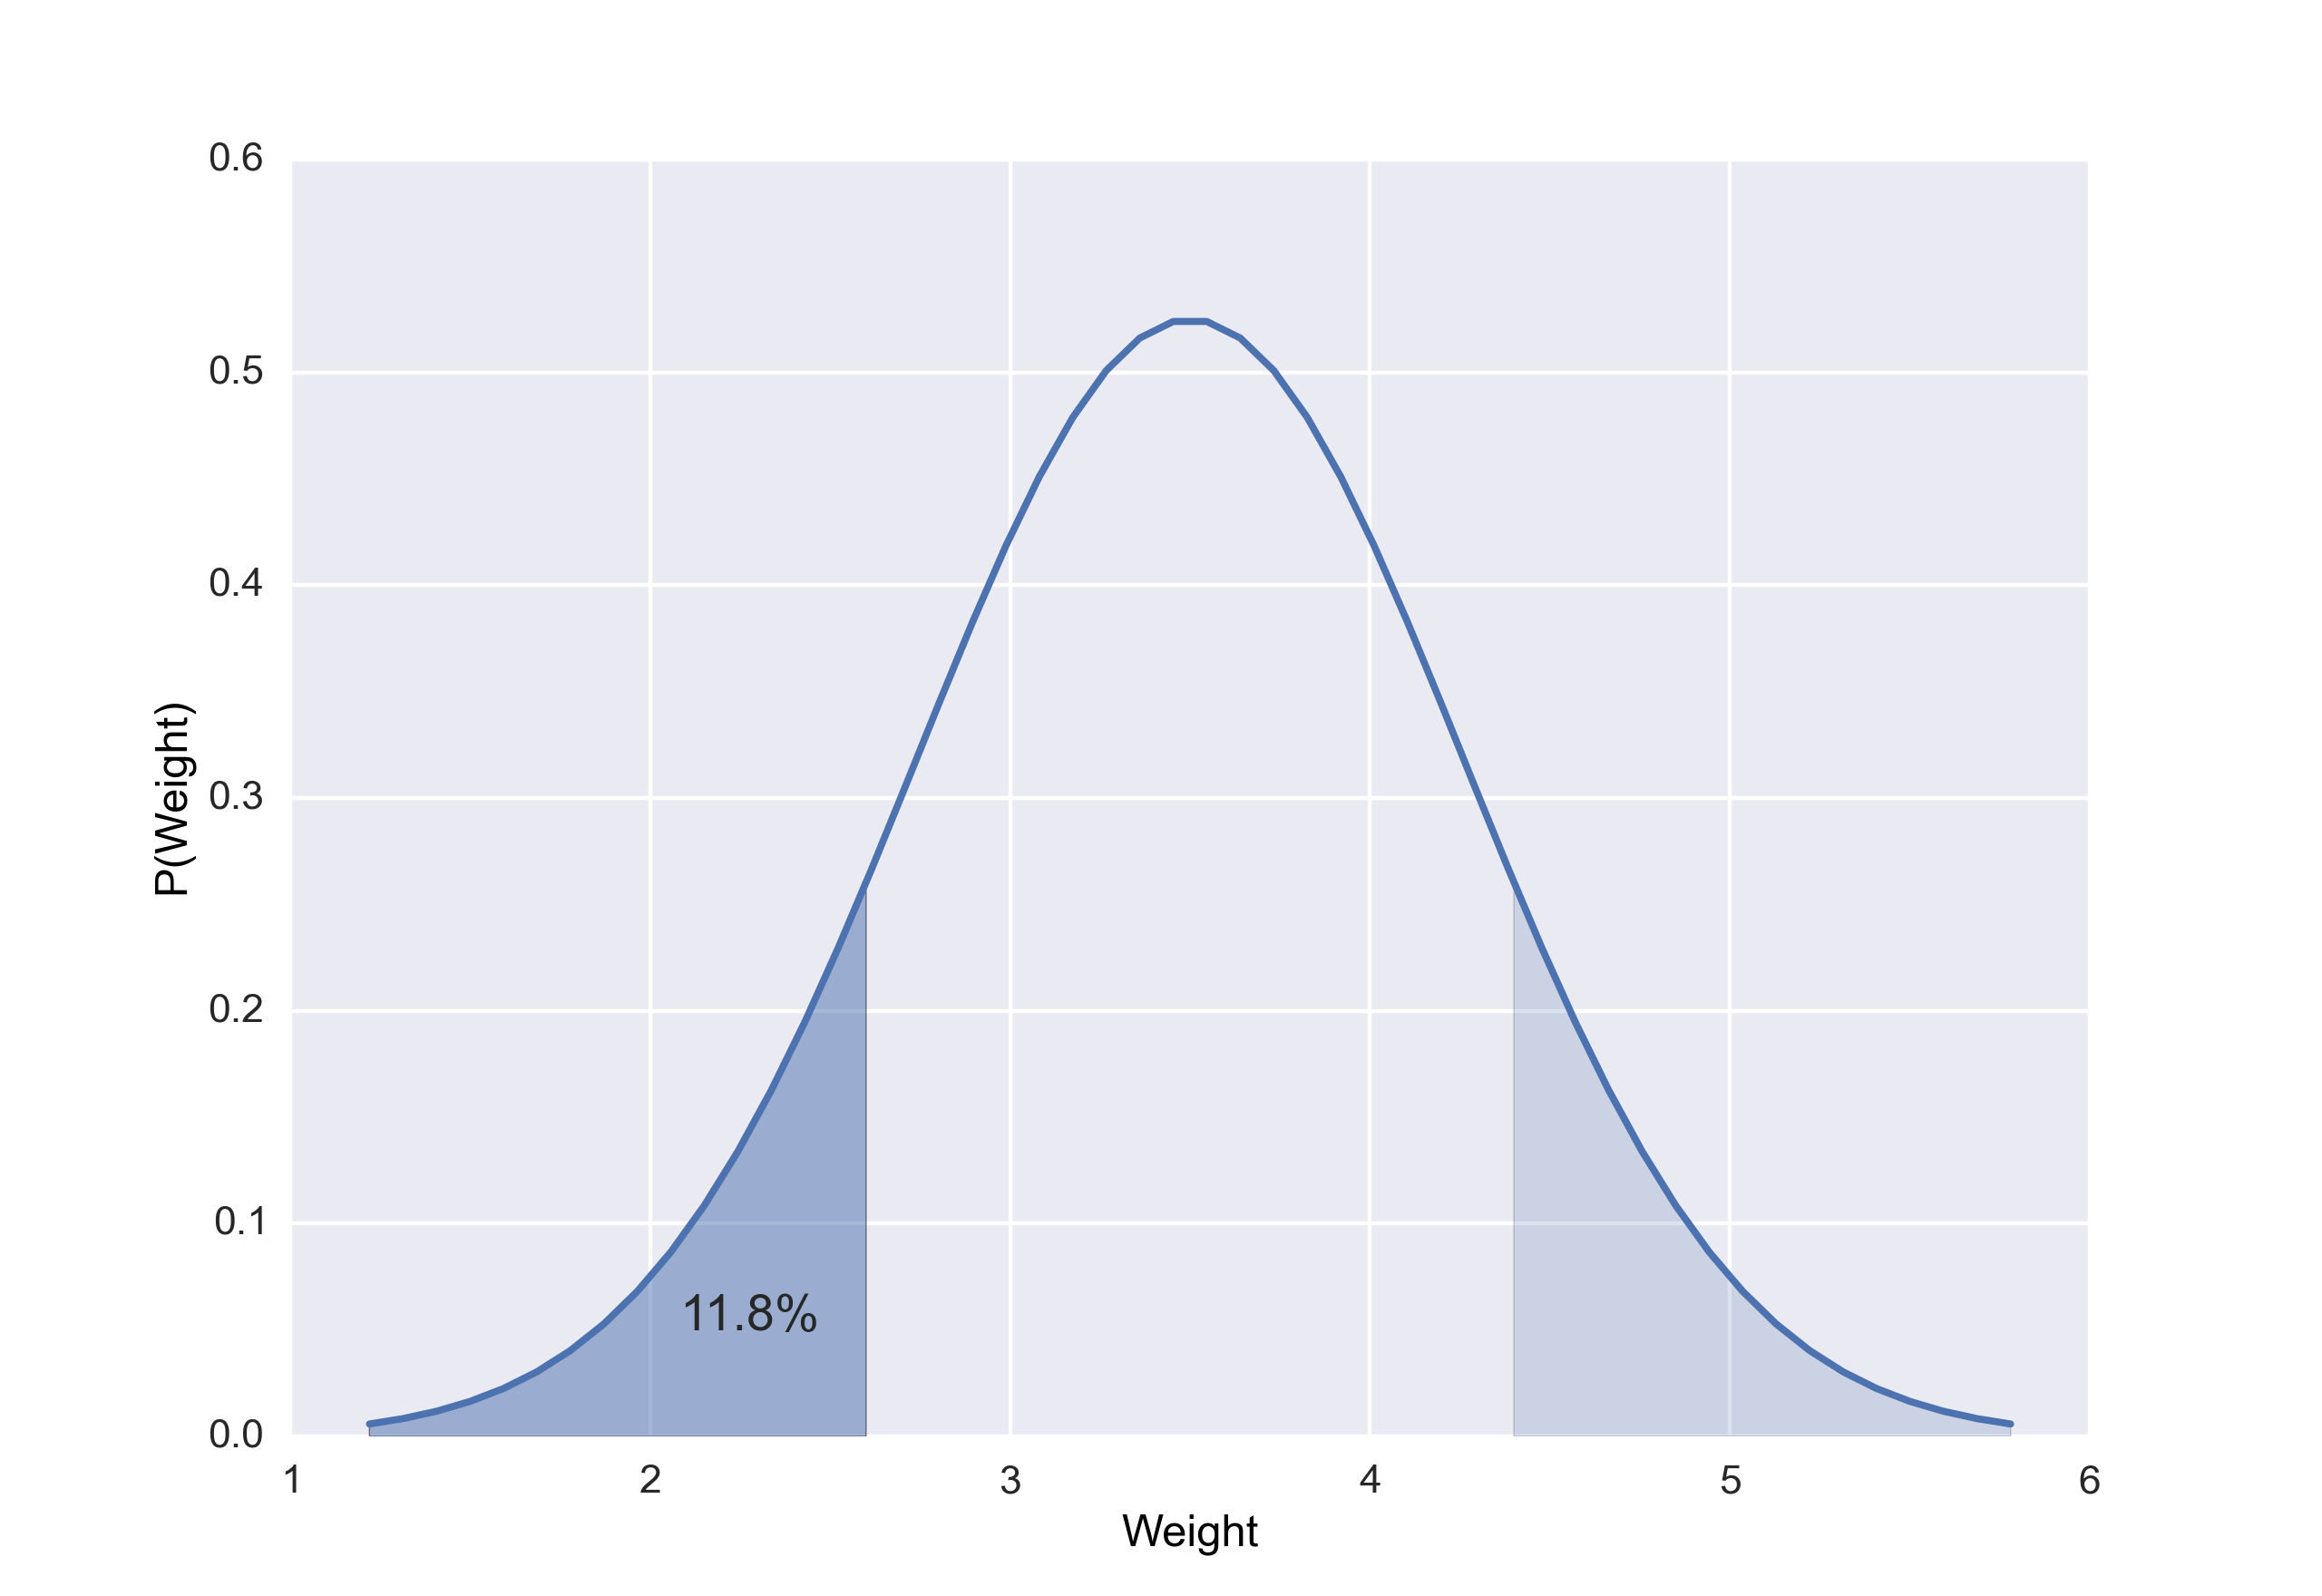
\includegraphics[width=0.75\textwidth]{../Images/pdf_checkValue.png}\\
  \caption{The chance that a healthy baby weighs 2.6 kg or less is 11.8\% (darker blue area). The chance that the difference from the mean is that much is twice that much, as the lighter blue area must be added.}\label{fig:pdf_checkValue}
\end{figure}

\subsection{Other Continuous Distributions}\label{sec:ContinuousDistributions} \index{general}{distributions!continuous}

The distributions you will encounter most frequently are:

\begin{itemize}
  \item \textbf{Normal distribution} - the "ideal" continuous probability distribution
  \item \textbf{t-distribution} - for sample distributions (What you will probably use most often.)
  \item \textbf{$\chi$-square distribution} - for describing  variability
  \item \textbf{F-distribution} - for comparing variability
\end{itemize}

In the following, we will describe these distributions in more detail.

\subsubsection{t Distribution}\index{general}{distributions!t-distribution}
For a small number of samples (ca.$<10$) from a normal distribution, the distribution of the mean deviates slightly from the normal distribution. The reason is that the sample mean does not coincide exactly with the population mean. This modified distribution is the \emph{t-distribution}, and converges for larger values towards the normal distribution (Fig. \ref{fig:t}).

If $\bar{x}$ is the sample mean, and $s$ the sample standard deviation, then

\begin{equation}\
  t = \frac{\bar{x}-\mu}{s/ \sqrt{n}}
\end{equation}

A very frequent application of the t-distribution is in the calculation of confidence intervals (Eq. \ref{eq:ci}):

\begin{lstlisting}
  In [28]: n = 20
  In [29]: alpha = 0.05
  In [30]: stats.t(20).ppf(1-alpha/2)
  Out[30]: 2.0859634472658364

  In [31]: stats.norm.ppf(1-alpha/2)
  Out[31]: 1.959963984540054
\end{lstlisting}
\emph{Calculating the t-values for confidence intervals, for n = 20 and $\alpha=0.05$. For comparison, I also calculate the corresponding value from the normal distribution.}

\begin{figure}
  \centering
  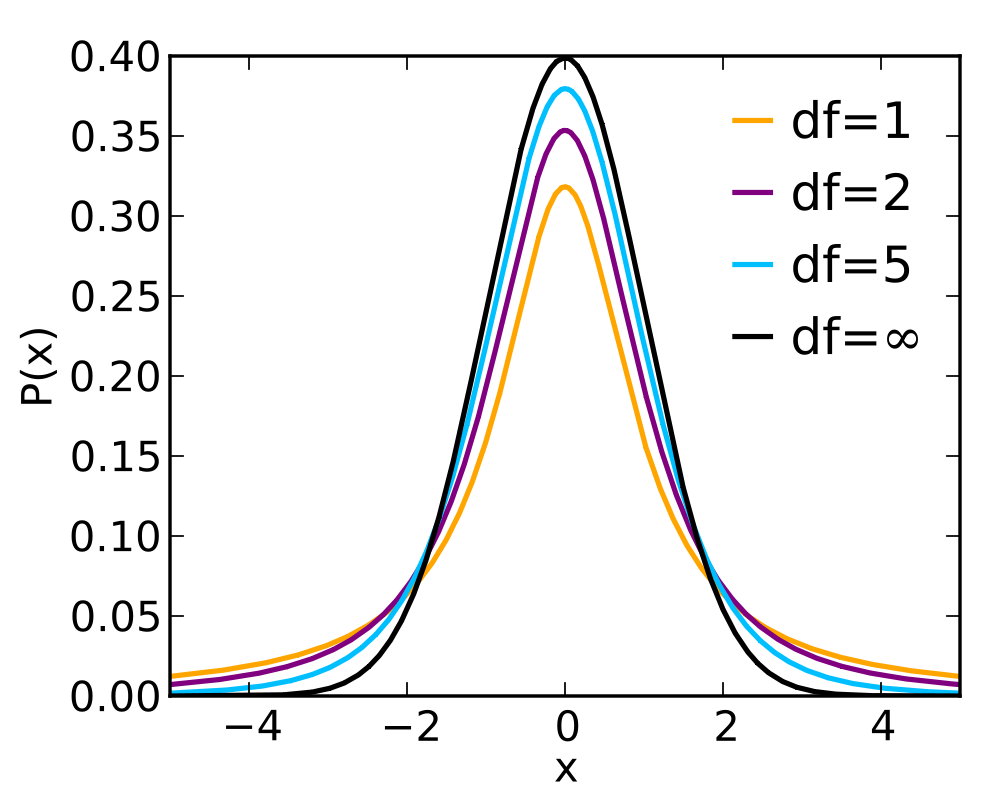
\includegraphics[width=0.5\textwidth]{../Images/Student_t_pdf.png}\\
  \caption{t Distribution}\label{fig:t}
\end{figure}

Since the t-distribution has longer tails than the normal distribution, it is much less sensitive to outliers (see Figure \ref{fig:ttest_stability}).

\begin{figure}
  \centering
  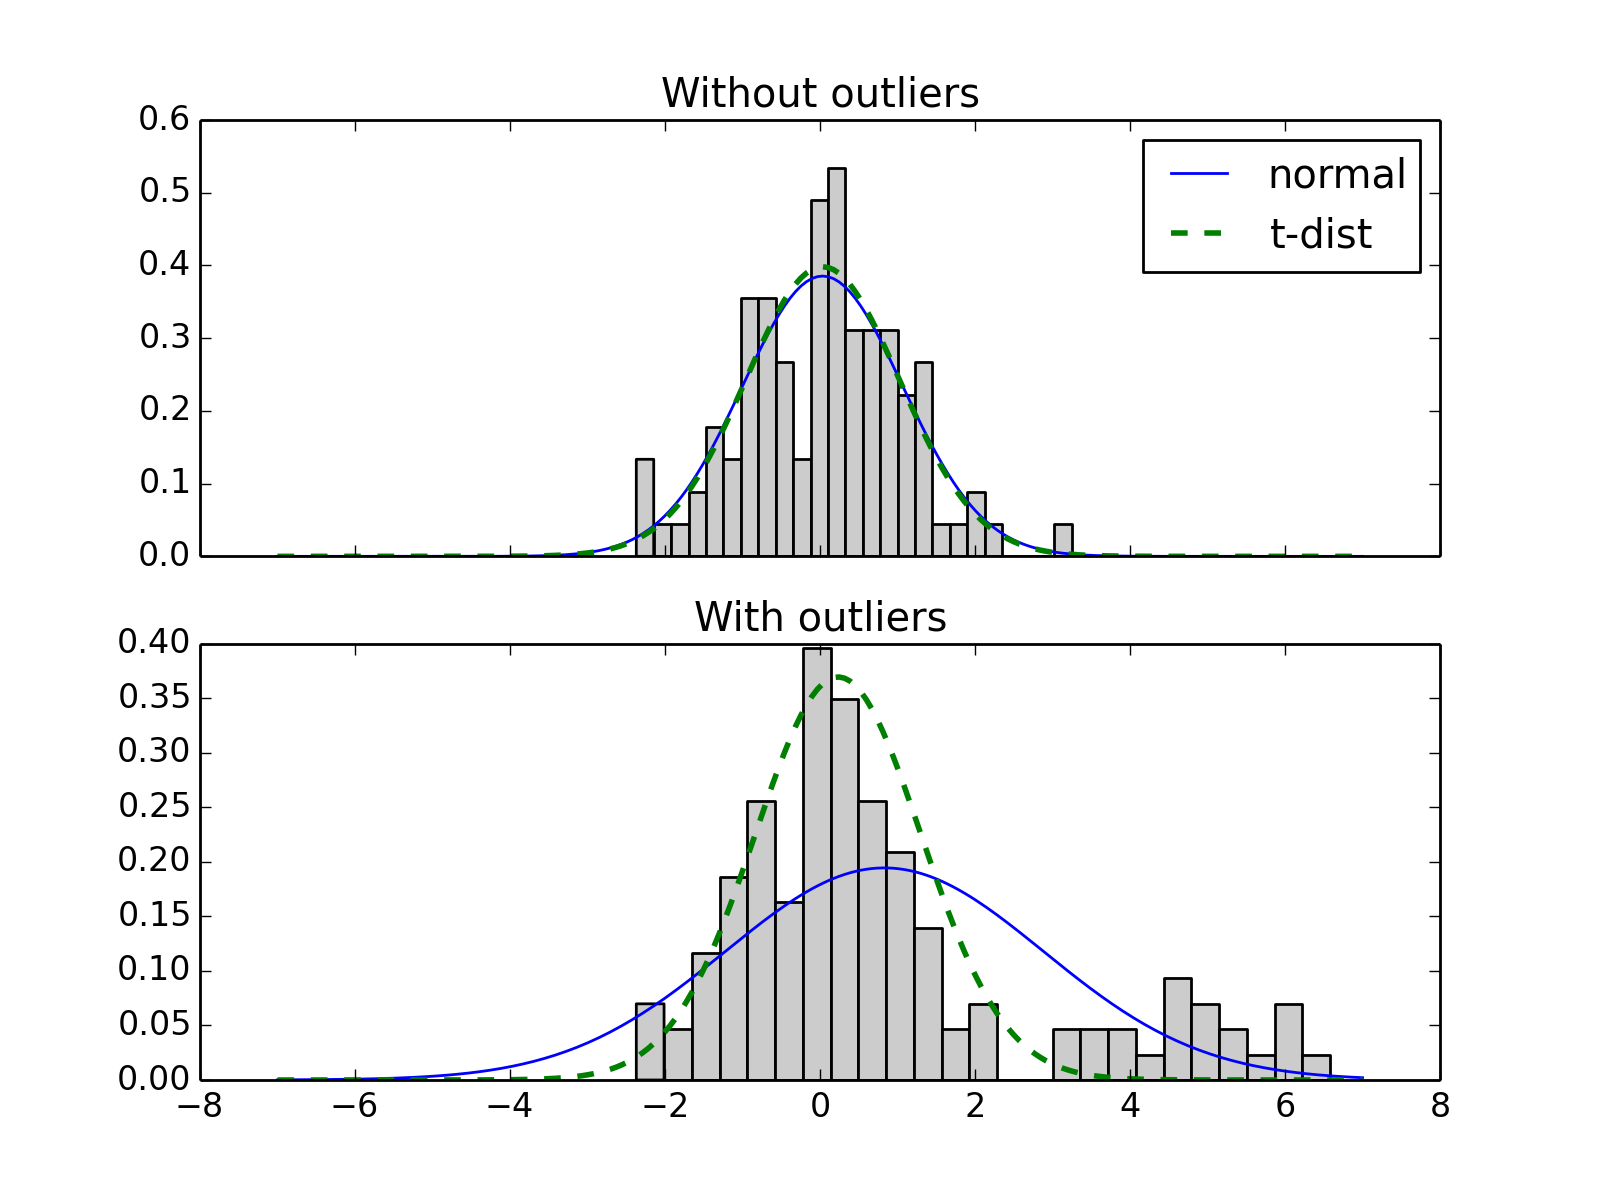
\includegraphics[width=0.75\textwidth]{../Images/ttest_stability.png}\\
  \caption{The t-distribution is much more robust against outliers than the normal distribution.}\label{fig:ttest_stability}
\end{figure}


\subsubsection{Chi-square Distribution}\index{general}{distributions!chi square}

The \emph{Chi-square distribution} is related to normal distribution in a simple way: If a random variable $X$ has a normal distribution ($X \in N(0,1)$), then $X^2$ has a chi-square distribution, with one degree of freedom ($X^2 \in \chi_{1}^2$). The sum squares of $n$ independent and standard normal random variables has a chi-square distribution with $n$ degrees of freedom:

\begin{equation}
    \sum\limits_{i = 1}^n {X_i^2} \in \chi_{n}^2
\end{equation}


\begin{figure}
  \centering
  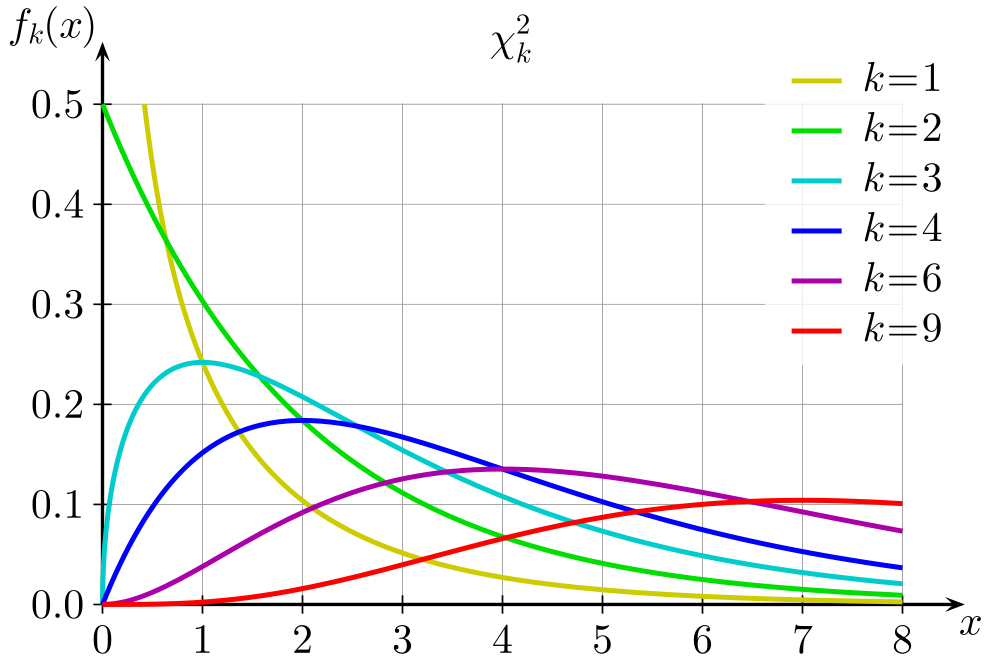
\includegraphics[width=0.5\textwidth]{../Images/ChiSquare_pdf.png}\\
  \caption{Chi-square Distribution}
\end{figure}

\textbf{Application Example}

A pill producer is ordered to deliver pills with a standard deviation of $\sigma=0.05$. From the next batch of pills you pick $n=13$ random samples. These samples $x_1, x_2, . . . , x_n$ have a weight of
3.04, 2.94, 3.01, 3.00, 2.94, 2.91, 3.02, 3.04, 3.09, 2.95, 2.99, 3.10, 3.02 g.

\emph{Question:} is the standard deviation larger than allowed?

\emph{Answer:}

Since the Chi-square distribution describes the distribution of the summed squares of random variates from a \emph{standard normal distribution}, we have to normalize our data before we calculate the corresponding CDF-value:

\begin{equation}
  1 - CD{F_{{\chi ^2}_{(n - 1)}}}\left( {\sum {(\frac{{x - \bar x}}{\sigma }} {)^2}} \right) = 0.1929
\end{equation}

\emph{Interpretation:} if the batch of pills is from a distribution with a standard deviation of $\sigma=0.05$, the likelihood of obtaining a chi-square value as large or larger than the one observed is about 19\%, so it is not atypical. In other words, the batch matches the expected standard deviation.

\subsubsection{F Distribution}\index{general}{distributions!F distribution}
Named after Sir Ronald Fisher, who developed the F distribution for use in determining critical values in ANOVAs (\emph{ANalysis Of VAriance}).  The cutoff values in an F table are found using three variables:

\begin{itemize}
  \item ANOVA numerator degrees of freedom
  \item ANOVA denominator degrees of freedom
  \item significance level
\end{itemize}

ANOVA compares the size of the variance between two different samples. This is done by dividing the larger variance over the smaller variance. The formula for the resulting \emph{F statistic} is:

\begin{equation}
    F(r_1, r_2) = \frac{\chi_{r1} ^2 /r_1}{\chi_{r2} ^2 /r_2}
\end{equation}

where $\chi_{r1}^2$ and $\chi_{r2}^2$ are the chi-square statistics of sample one and two respectively, and $r_1$ and $r_2$ are their degrees of freedom, i.e. the number of observations.

\paragraph{F-Test of Equality of Variances}
If you want to investigate whether two groups have the same variance, you have to calculate the ratio of the sample standard deviations squared:

\begin{equation}
  F = \frac{S_x^2}{S_y^2}
\end{equation}

where $S_x$ ist he sample standard deviation of the first sample, and $S_y$ the sample standard deviation for the second sample.

\textbf{Application Example}

Take for example the case that you want to compare two methods to measure eye movements. The two methods
can have different accuracy and different precision. With your test you want to
determine if the precision of the two methods is equivalent, or if one
method is more precise than the other.

\begin{figure}
  \centering
  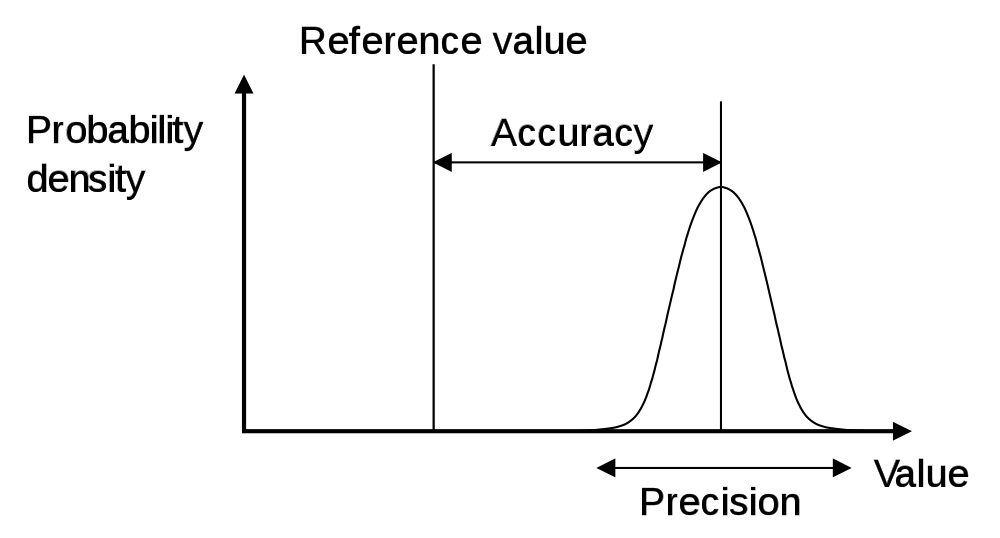
\includegraphics[width=0.5\textwidth]{../Images/Accuracy_and_precision.png}\\
  \caption{Accuracy and precision of a measurement are two different characteristics!}
\end{figure}

When you look 20 deg to the right, you get the following results:
Method 1: [20.7,  20.3,  20.3,  20.3,  20.7,  19.9,  19.9,  19.9,  20.3,
        20.3,  19.7,  20.3]
Method 2: [ 19.7,  19.4,  20.1,  18.6,  18.8,  20.2,  18.7,  19. ]

The F statistic is $F = 0.494$, and has $n-1$ and $m-1$ degrees of freedom, where $n$ and $m$ are the number of recordings with each method. The code sample below shows that the F statistic is close to the center of the distribution, so we cannot reject the hypothesis that the two methods have the same precision.

\begin{lstlisting}
  In [1]:  method1 = array([20.7,  20.3,  20.3,  20.3,  20.7,  19.9,  19.9,  19.9,  20.3,
        20.3,  19.7,  20.3])
  In [2]:  method2 = array([ 19.7,  19.4,  20.1,  18.6,  18.8,  20.2,  18.7,  19. ])
  In [3]:  fval = var(method1, ddof=1)/var(method2, ddof=1)
  In [4]:  fd = stats.f(len(method2)-1,len(method2)-1)
  In [5]:  p = fd.cdf(fval)
  In [6]:  print p
  Out[6]:  0.041
  In [7]:  if (p<0.025) or (p>0.975):
              print 'There is a significant difference between the two distributions.'
\end{lstlisting}

\begin{figure}
  \centering
  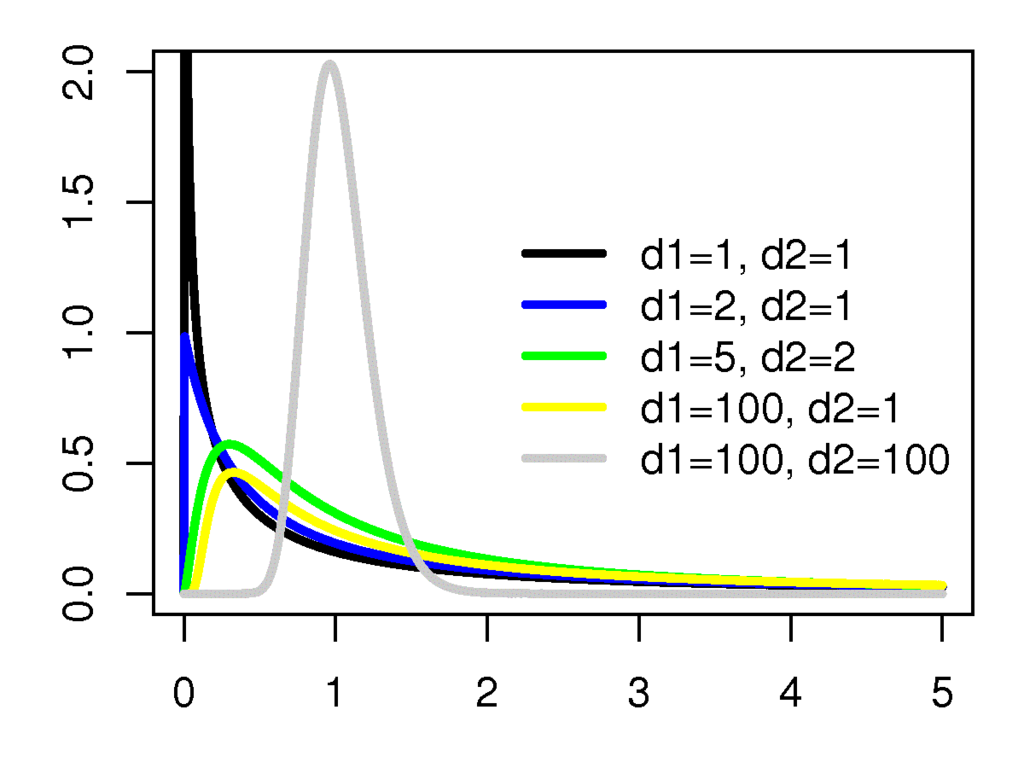
\includegraphics[width=0.5\textwidth]{../Images/F_distributionPDF.png}\\
  \caption{F Distribution}
\end{figure}


\subsubsection{Lognormal Distribution}\index{general}{distributions!lognormal}

In some circumstances a set of data with a positively skewed distribution can be transformed into a symmetric distribution by taking logarithms. Taking logs of data with a skewed distribution will often give a distribution that is near to normal (see Figure \ref{fig:lognormal}).

\begin{figure}
\centering
\begin{subfigure}{.5\textwidth}
  \centering
  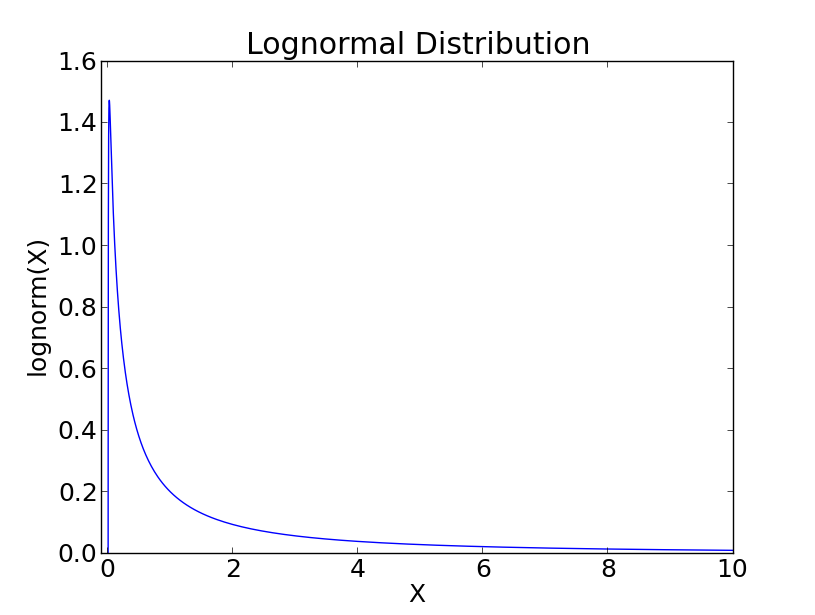
\includegraphics[width=.8\linewidth]{../Images/LogNormal_Linear.png}
  \caption{Plotted against a linear abscissa.}
  \label{fig:Lognormal_Sub1}
\end{subfigure}%
\begin{subfigure}{.5\textwidth}
  \centering
  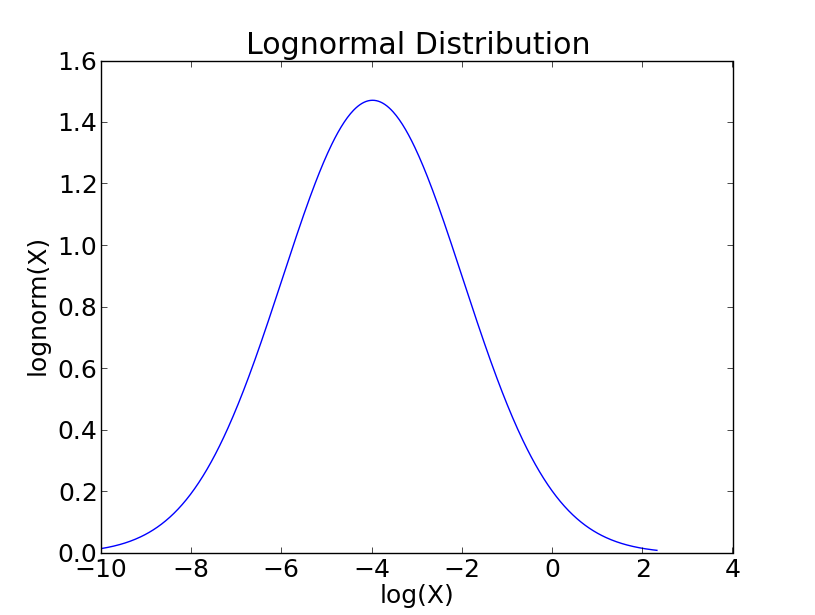
\includegraphics[width=.8\linewidth]{../Images/LogNormal_Logarithmic.png}
  \caption{Plotted against a logarithmic abscissa.}
  \label{fig:Lognormal_Sub2}
\end{subfigure}
\caption{Lognormal distribution}
\label{fig:lognormal}
\end{figure}

\subsubsection{Weibull Distribution}\index{general}{distributions!weibull}

The Weibull distribution is the most commonly used distribution for modeling reliability data or "survival" data. It has two parameters, which allow it to handle increasing, decreasing or constant failure-rates (see Figure \ref{fig:weibull}).
It is defined as

\begin{equation}\label{eq_weibull}
f_x (x) =
  \begin{cases}
    \frac{k}{\lambda}\left(\frac{x}{\lambda}\right)^{k-1}e^{-(x/\lambda)^{k}} & x\geq0 ,\\
    0 & x<0 ,
    \end{cases}
\end{equation}

where $k > 0$ is the \emph{shape parameter }and $\lambda > 0$ is the \emph{scale parameter }of the distribution. Its complementary cumulative distribution function is a stretched exponential function.

If the quantity x is a "time-to-failure", the Weibull distribution gives a distribution for which the failure rate is proportional to a power of time. The shape parameter, k, is that power plus one, and so this parameter can be interpreted directly as follows:

\begin{itemize}
  \item  A value of $k < 1$ indicates that the failure rate decreases over time. This happens if there is significant "infant mortality", or defective items failing early and the failure rate decreasing over time as the defective items are weeded out of the population.

  \item  A value of $k = 1$ indicates that the failure rate is constant over time. This might suggest random external events are causing mortality, or failure.
  \item  A value of $k > 1$ indicates that the failure rate increases with time. This happens if there is an "aging" process, or parts that are more likely to fail as time goes on.
\end{itemize}

In the field of materials science, the shape parameter k of a distribution of strengths is known as the Weibull modulus.

\begin{figure}
  \centering
  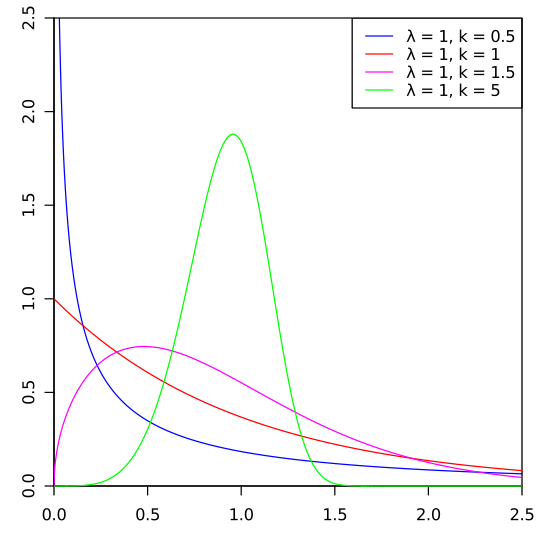
\includegraphics[width=0.5\textwidth]{../Images/Weibull_PDF.png}\\
  \caption{Weibull Distribution}\label{fig:weibull}
\end{figure}


\subsubsection{Exponential Distribution}\index{general}{distributions!exponential}

For a stochastic variable X with an \emph{exponential distribution}, the probability distribution function is:
\begin{equation}\label{eq_exponential}
f_x (x) =
  \begin{cases}
\lambda e^{- \lambda x}, & \mbox{if } x \ge 0 \\
0, & \mbox{if } x < 0
\end{cases}
\end{equation}

The exponential PDF is shown in Figure \ref{fig:exponential}
\begin{figure}
  \centering
  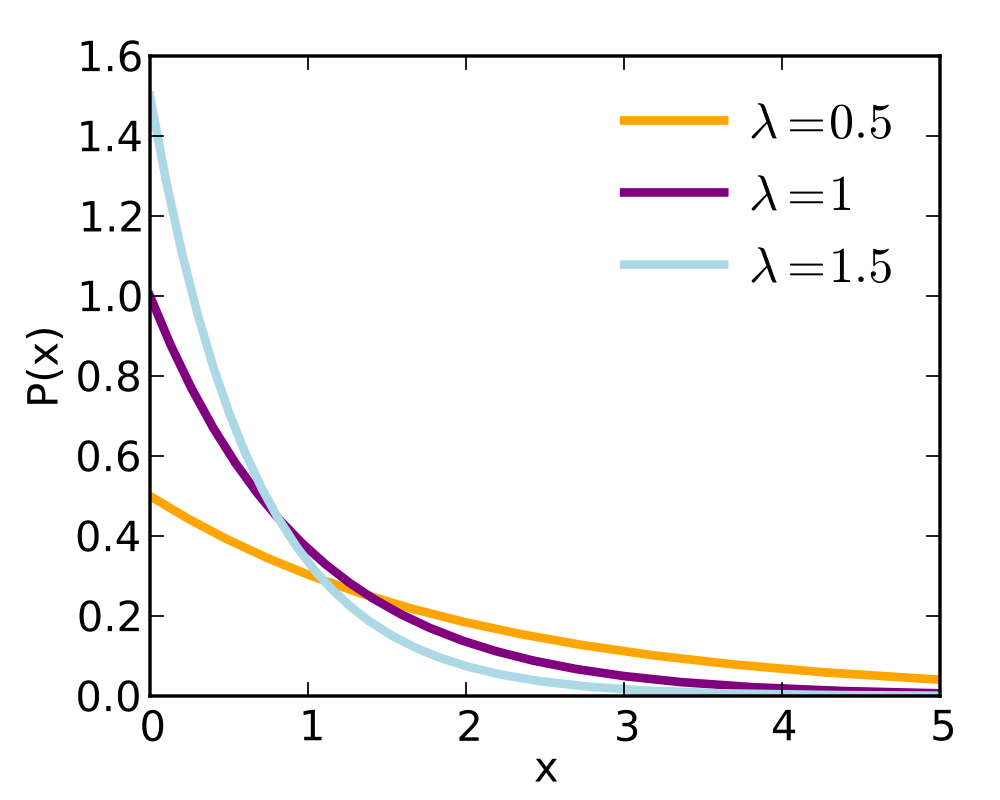
\includegraphics[width=0.5\textwidth]{../Images/Exponential_pdf.png}\\
  \caption{Exponential Distribution}\label{fig:exponential}
\end{figure}


\subsubsection{Uniform Distribution}\index{general}{distributions!uniform}

This is a simple one: an even probability for all data values (Figure \ref{fig:uniform}). Not very common for real data.

\begin{figure}
  \centering
  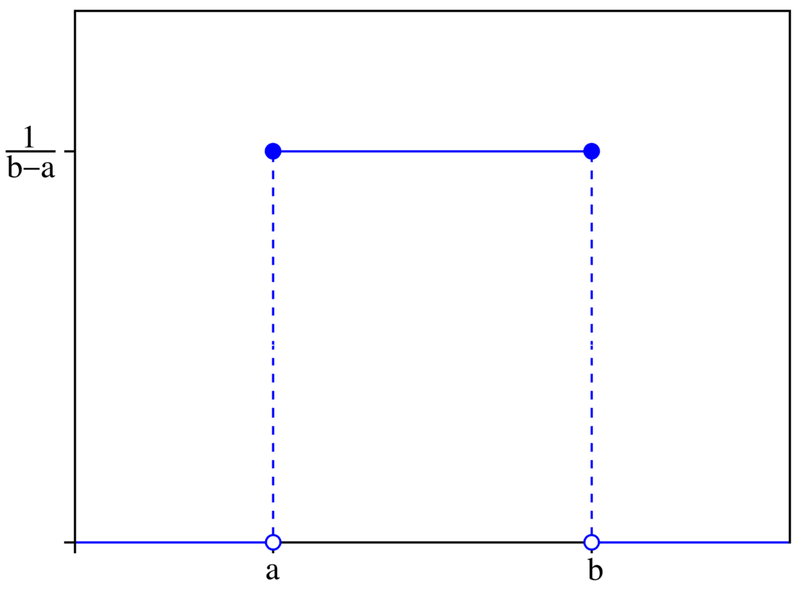
\includegraphics[width=0.5\textwidth]{../Images/Uniform_Distribution_PDF.png}\\
  \caption{Uniform Distribution} \label{fig:uniform}
\end{figure}

\subsubsection{Programs: Continuous Distribution Functions}

Working with distribution functions in Python takes a bit to get used to. But once you get the concept, it is marvellously easy. In my opinion, the most logical way is first to define the function, with all the parameters that it requires; and then, to use the methods of this function, e.g. $pdf$, or $cdf$:

\begin{lstlisting}
  In [1]: from scipy import stats
  In [2]: myDF = stats.norm(5,3)
  In [3]: x = linspace(-5, 15, 101)
  In [4]: y = myDF.pdf(x)
\end{lstlisting}

\PyImg "distributionContinuous.py" (p \pageref{py:continuous}) shows different continuous distribution functions.
\index{python}{distributionContinuous}

\subsection{Discrete Distributions}\index{general}{distributions!discrete}

While the functions describing continuous distributions are referred to as \emph{probability density functions}, discrete distributions are described by \emph{probability mass functions}.

\subsubsection{Binomial Distribution}\index{general}{distributions!binomial}
The Binomial is associated with the question "Out of a given number of trials, how many will succeed?" Some example questions that are modeled with a Binomial distribution are:
\begin{itemize}
  \item Out of ten tosses, how many times will this coin land ''heads''?
  \item From the children born in a given hospital on a given day, how many of them will be girls?
  \item How many students in a given classroom will have green eyes?
  \item How many mosquitos, out of a swarm, will die when sprayed with insecticide?
\end{itemize}

  We conduct $n$ repeated experiments where the probability of success is given by the parameter $p$ and add up the number of successes. This number of successes is represented by the random variable $X$.  The value of $X$ is then between 0 and $n$.

When a random variable X has a Binomial Distribution with parameters $p$ and $n$ we write it as $\,X \sim Bin(n,p)$ or $\,X \sim B(n,p)$ and the probability mass function is given at $X=k$ by the equation:

\begin{equation}
    P\left[X = k\right] = \begin{cases} {n \choose k} p^k \left(1-p\right)^{n-k}\ & 0 \le k \le n \\ 0 & \mbox{otherwise} \end{cases} \quad 0 \leq p \leq 1, \quad n \in \mathbb{N}
\end{equation}

where ${n \choose k}={n! \over k!(n-k)!}$

\begin{figure}
  \centering
  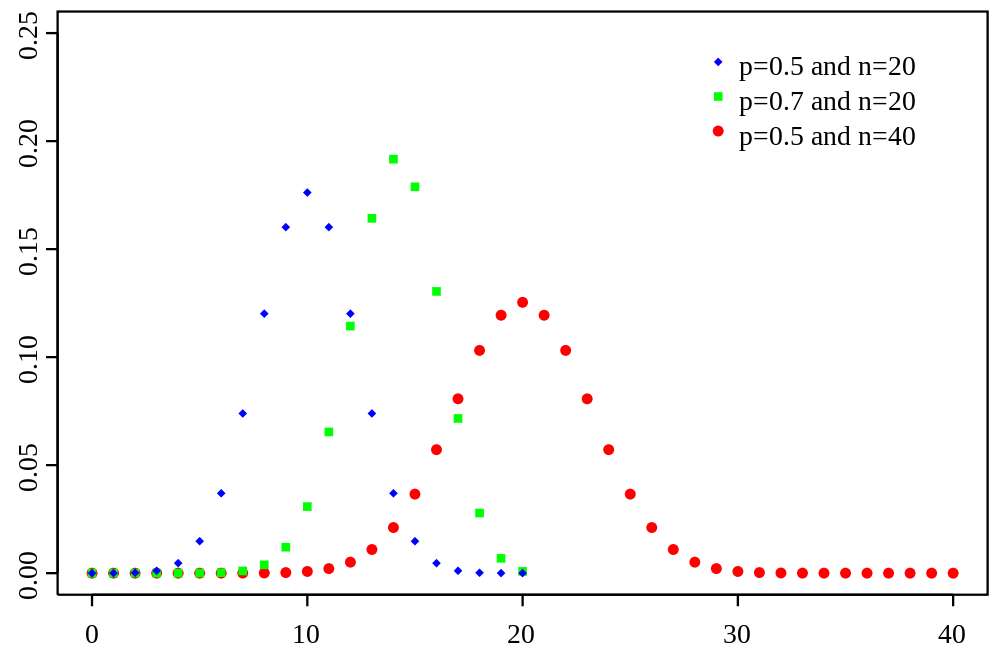
\includegraphics[width=0.75\textwidth]{../Images/Binomial_distribution_pmf.png}\\
  \caption{Binomial Distribution}
\end{figure}

The binomial distribution for $n = 1$ is sometimes referred to as \emph{Bernoulli Distribution}. \index{general}{distributions!Bernoulli}

\subsubsection{Poisson Distribution}\index{general}{distributions!poisson}

Any French speaker will notice that "Poisson" means "fish", but really there's nothing fishy about this distribution. It's actually pretty straightforward. The name comes from the mathematician Siméon-Denis Poisson (1781-1840).

The Poisson Distribution is ''very similar'' to the Binomial Distribution. We are examining the number of times an event happens. The difference is subtle. Whereas the Binomial Distribution looks at how many times we register a success over a fixed total number of trials, the Poisson Distribution measures how many times a discrete event occurs, over a period of continuous space or time. There isn't a "total" value n. As with the previous sections, let's examine a couple of experiments or questions that might have an underlying Poisson nature.

\begin{itemize}
  \item How many pennies will I encounter on my walk home?
  \item How many children will be delivered at the hospital today?
  \item How many products will I sell after airing a new television commercial?
  \item How many mosquito bites did you get today after having sprayed with insecticide?
  \item How many defects will there be per 100 metres of rope sold?
\end{itemize}

What's a little different about this distribution is that the random variable $X$ which counts the number of events can take on \emph{any non-negative integer} value. In other words, I could walk home and find no pennies on the street. I could also find one penny. It's also possible (although unlikely, short of an armored-car exploding nearby) that I would find 10 or 100 or 10,000 pennies.

Instead of having a parameter p that represents a component probability like in the Binomial distribution, this time we have the parameter "lambda" or $\lambda$ which represents the "average or expected" number of events to happen within our experiment. The probability mass function of the Poisson is given by

\begin{equation}
  P(X=k)=\frac{e^{-\lambda}\lambda^k}{k!}
\end{equation}.


\begin{figure}
  \centering
  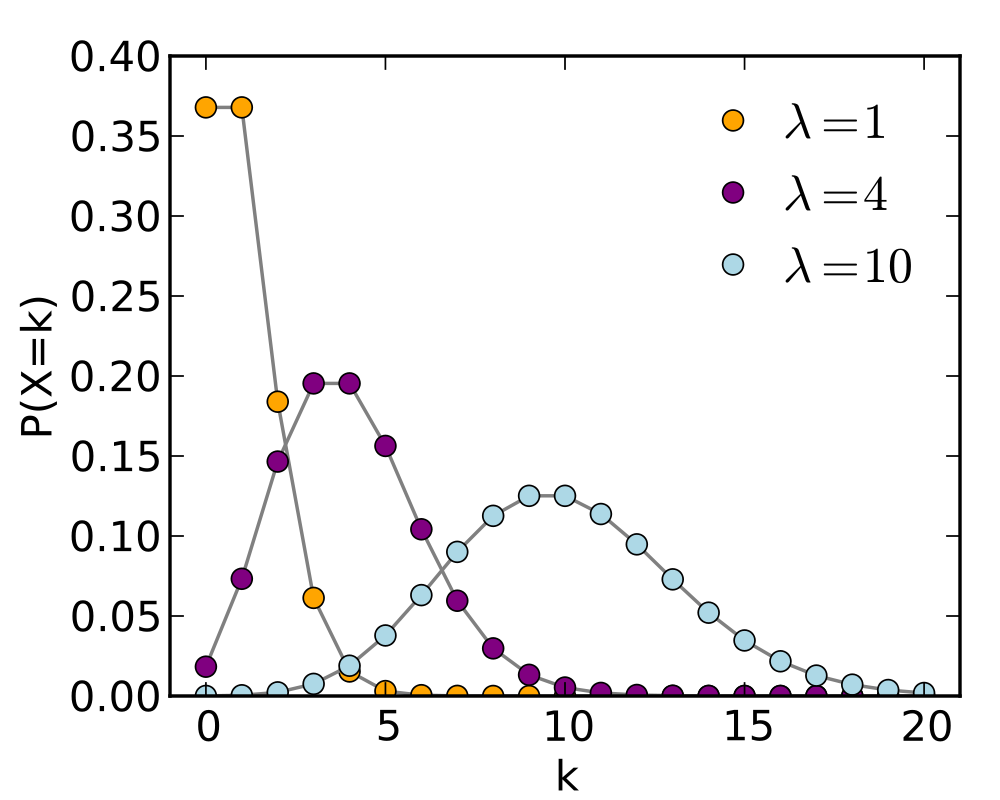
\includegraphics[width=0.5\textwidth]{../Images/Poisson_pmf.png}\\
  \caption{Poisson Distribution}
\end{figure}

\subsubsection{Programs: Discrete Distribution Functions} \index{general}{distributions!discrete}

\PyImg "distributionDiscrete.py" (p \pageref{py:discrete}) shows different continuous distribution functions.
\index{python}{distributionDiscrete}
%(Lecture 7)

\section{Exercises}

\subsection{Python}
\begin{enumerate}
  \item Create an numpy-array, containing the data 1,2,3,...,10. Calculate mean and sample(!)-standard deviation.
    (Correct answer: 3.03)
\end{enumerate}

\subsection{Distributions}


\begin{enumerate}
  \item  Generate and plot the Probability Density Function (PDF) of a normal distribution, with a mean of 5 and a standard deviation of 3.
  \item  Generate 1000 random data from this distribution.
  \item  Calculate the standard error of the mean of these data.
    (Correct answer: ca. 0.096)

  \item  Plot the histogram of these data.
  \item  From the PDF, calculate the interval containing 95\% of these data.
    (Correct answer: [ -0.88, 10.88])
\end{enumerate}

\subsection{Analysis}
\begin{enumerate}
  \item
  \begin{enumerate}
    \item Read in the data from 'Data\textbackslash amstat\textbackslash calcium.dat.txt'.
    \item Check for erroneous entries.
    \item Check the Alkaline Phosphatase levels for normality. Use a log-transform on the data, and re-check.
  \end{enumerate}

\end{enumerate}

\subsection{Continuous Distributions }
\begin{enumerate}
    \item \textbf{Normal Distribution:} Your doctor tells you that he can use hip implants for surgery even if they are 1 mm bigger or smaller than the specified size. And your financial officer tells you that you can discard 1 out of 1000 hip implants, and still make a profit.

        What is the required standard deviation for the producer of the hip implants, to simultaneously satisfy both requirements?
        (Correct answer: $\sigma=0.304 mm$)
    \item \textbf{T-Distribution:} Measuring the weight of your colleagues, you have obtained the following weights: 52, 70, 65, 85, 62, 83, 59 kg.
    Calculate the corresponding mean, and the 99\% confidence interval for the mean. Note: with n values you have n-1 DOF for the t-distribution.
    (Correct answer: 68.0 +/- 17.2 kg)

    \item \textbf{Chi-square Distribution:} Create 3 normally distributed datasets (mean = 0, SD = 1), with 1000 samples each. Then square them, sum them (so that you have 1000 data-points), and create a histogram with 100 bins. This should be similar to the curve for the Chi-square distribution, with 3 DOF (i.e. it should come down at the left, see figure below).
    \begin{figure}
      \centering
      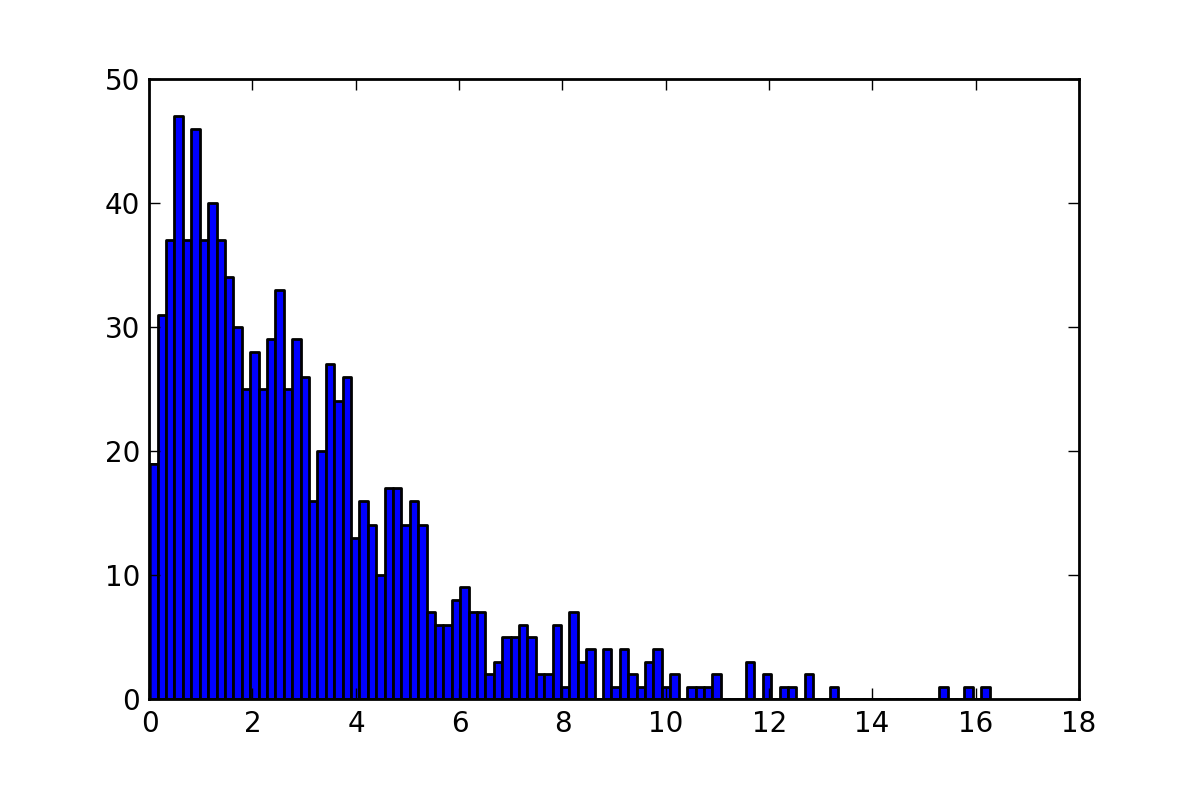
\includegraphics[width=0.5\textwidth]{../Images/chi2_3dof.png}\\
      \caption{chi2 distribution with 3 degrees of freedom.}\label{fig:chi23dof}
    \end{figure}

    \item \textbf{F Distribution:} You have two apple trees. There are three apples from the first tree that weigh 110, 121 and 143 grams respectively, and four from the other which weigh 88, 93, 105 and 124 grams respectively. Are the variances from the two trees different?
    Note: calculate the corresponding F-value, and check if the CDF for the corresponding F-distribution is $<0.025$.
    (Correct answer: no)
\end{enumerate}
\subsection{Discrete Distributions }

\begin{enumerate}
    \item \textbf{Binomial Distribution} "According to research, pure blue eyes in Europe approach greatest frequency in Finland, Sweden and Norway(at 72\%), followed by Estonia, Denmark(69\%); Latvia, Ireland(66\%); Scotland(63\%); Lithuania(61\%); The Netherlands(58\%); Belarus, England(55\%); Germany(53\%); Poland, Wales(50\%); Russia, The Czech Republic(48\%); Slovakia(46\%); Belgium(43\%); Austria, Switzerland, Ukraine(37\%); France, Slovenia(34\%); Hungary(28\%); Croatia(26\%); Bosnia and Herzegovina(24\%); Romania(20\%); Italy(18\%); Serbia, Bulgaria(17\%); Spain(15\%); Georgia, Portugal(13\%); Albania(11\%); Turkey and Greece(10\%). Further analysis shows that the average occurrence of blue eyes in Europe is 34\%, with 50\% in Northern Europe and 18\% in Southern Europe."

    If we have 15 Austrian students in the class-room, what ist the chance of finding 3, 6, or 10 students with blue eyes?
    (Correct answer: 9\%, 20.1\%, and 1.4\%)

    \item \textbf{Poisson Distribution} On the streets of Austria there were 62 fatal accidents in 2012. Assuming that those are evenly distributed, we have on average
    62 /(365/7)=1.19 fatal accidents per week. How big is the chance that in a given week there are no, 2, or 5 accidents?
    (Correct answer: 30.5\%, 21.5\%, 0.6\% )
\end{enumerate}

\chapter{Statistical Tests}

\section{Hypothesis tests}\label{sec:hypotheses} \index{general}{hypotheses}

Statistical evaluations are based on the initially often counterintuitive procedure of \emph{hypothesis tests}. A hypothesis test is a standard format for assessing statistical evidence. It is ubiquitous in scientific literature, most often appearing in the form of statements of \emph{statistical significance} and quotations like $"p<0.01"$ that pepper scientific journals. Thereby you proceed as follows: you

\begin{itemize}
  \item   state your hypothesis.
  \item   decide which value you want to test your hypothesis on.
  \item   calculate the \emph{probability p} that you find the given value, assuming that your hypothesis is true
\end{itemize}

The first hypothesis is referred to as \emph{null-hypothesis}, since we assume that there is \emph{null} difference between the hypothesis and the result. The found probability for a specific target value is the \emph{p-value} that you typically find in the literature. If $p<0.05$, the difference between your sample and the value that you check is \emph{significant}. If $p<0.001$, we speak of a \emph{highly significant} difference.

\textbf{Example 1: } Let us compare the weight of two groups of subject. Then the \emph{null hypothesis} is that there is \emph{null} difference in the weight between the two groups. If a statistical comparison of the weight produces a p-value of 0.03, this means that \emph{the probability that the null hypothesis is correct is 0.03, or 3\%}. Since this probability is quite low, we say that \emph{there is a significant difference between the weight of the two groups}.

\textbf{Example 2: } If we want to check the assumption that the mean value of a group is 7, then the null hypothesis would be: \emph{"We assume that there is null difference between the mean value in our poulation and the value 7."}

\subsection{Types of Error}
In hypothesis testing, two types of errors can occur:

\subsubsection{Type I errors} \index{general}{error!Type I} \index{general}{power}
These are errors, where you get a significant result despite the fact that the hypothesis is true. The likelihood of a Type I error is commonly indicated with $\alpha$, and \emph{is set before you start the data analysis}.

For example, assume that the population of young Austrian adults has a mean IQ of 105 (i.e. we are smarter than the rest) and a standard deviation of 15. We now want to check if the average FH student in Linz has the same IQ as the average Austrian, and we select 20 students. We set $\alpha=0.05$, i.e. we set our significance level to 95\%.
Let us now assume that the average student has in fact the same IQ as the average Austrian. If we repeat our study 20 times, we will find one of those 20 times that our sample mean is significantly different from the Austrian average IQ. Such a finding would be a false result, despite the fact that our assumption is correct, and would constitute a \emph{type I error}.

\subsubsection{Type II errors and Test Power}\index{general}{error!Type II}
If we want to answer the question "How much chance do we have to reject the null hypothesis when the alternative is in fact true?" Or in other words, "What’s the probability of detecting a real effect?" we are faced with a different problem. To answer these questions, we need an \emph{alternative hypothesis}.

For the example given above, an \emph{alternative hypothesis} could be: "We assume that our population has a mean value of 6."

A \emph{Type II error} is an error, where you do \emph{not} get a significant result, despite the fact that the null-hypothesis is false. The probability for this type of error is commonly indicated with $\beta$. The \emph{power} of a statistical test is defined as $(1-\beta)*100$, and is the chance of correctly accepting the alternate hypothesis. Figure \ref{fig:power1} shows the meaning of the \emph{power} of a statistical test. Note that for finding the power of a test, you need an alternative hypothesis.

\subsection{Sample Size}\index{general}{sample size}
The power of a statistical test depends on four factors:

\begin{enumerate}
  \item  $\alpha$, the probability for Type I errors
  \item  $\beta$, the probability for Type II errors ( $\Rightarrow$ power of the test)
  \item  $d$, the \emph{effect size}, i.e. the magnitude of the investigated effect relative to $\sigma$, the standard deviation of the sample
  \item  $n$, the sample size
\end{enumerate}

Only 3 of these 4 parameters can be chosen, the $4^{th}$ is then automatically fixed.

The absolute size of the difference $D$ between mean treatment outcomes that will answer the clinical question being posed is often called \emph{clinical significance} or \emph{clinical relevance}.

\begin{figure}[!ht]
  \centering
  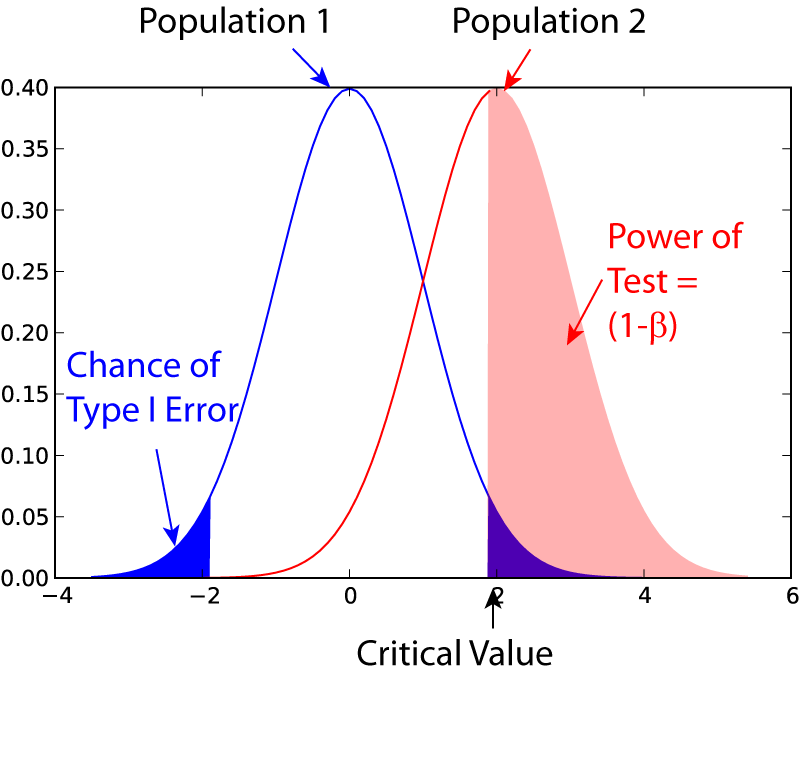
\includegraphics[width=0.5\textwidth]{../Images/power1.png}\\
  \caption{\emph{Power} of a statistical test, for comparing the mean value of two given distributions.}\label{fig:power1}
\end{figure}

\begin{figure}[!ht]
  \centering
  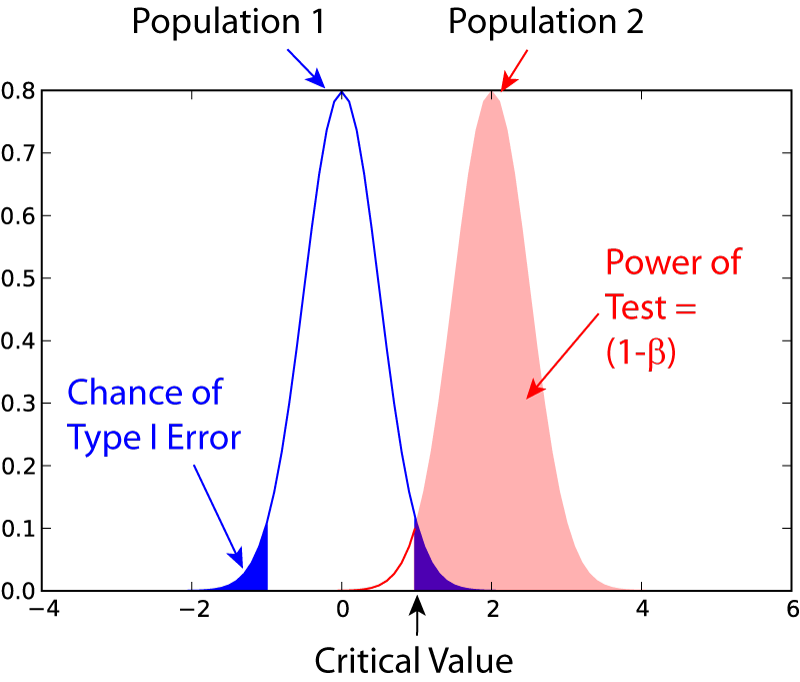
\includegraphics[width=0.5\textwidth]{../Images/power2.png}\\
  \caption{Effect of an increase in sampling size on the power of a test.}\label{fig:power2}
\end{figure}

\subsubsection{Examples for some special cases}

For a test on one mean, this leads to a \emph{minimum sample number} of

\begin{equation}
  n = \frac{{({z_{1 - \alpha /2}} + {z_{1 - \beta }})}^2}{d^2}
\end{equation}

Here z is the standardized normal variable (see also chapter \ref{sec:normalDistribution})

\begin{equation}
  z = \frac{x-\mu}{\sigma} .
\end{equation}

and $d = \frac{D}{\sigma}$ the effect size.

For finding a difference between two normally distributed means, the minimum number of samples we need in each group to detect an absolute difference $D$ is

\begin{equation}
  {n_1} = {n_2} = \frac{{({z_{1 - \alpha /2}} + {z_{1 - \beta }})}^2(\sigma _1^2 + \sigma _2^2)}{D^2} .
\end{equation}

\subsubsection{Programs: SampleSize}

\PyImg "sampleSize.py" (p \pageref{py:sampleSize}): sample size calculation for normally distributed groups.
\index{python}{sampleSize}


\subsection{The "p-value fallacy"}

p values are often used to measure evidence against a hypothesis. Unfortunately, they are often incorrectly viewed as an error probability for rejection of the hypothesis, or, even worse, as the posterior probability (i.e. after the data have been collected) that the hypothesis is true. As an example, take the case where the alternative hypothesis is that the mean is just a fraction of one standard deviation larger than the mean under the null hypothesis: in that case, a sample that produces a p-value of 0.05 may just as likely be produced if the the alternative hypothesis is true as if the null hypothesis is true!

\cite{sellke2001} have investigated this question in detail, and recommend to use a "calibrated p-value" to estimate the probability of making a mistake when rejecting the null hypothesis, when the data produce a p-value $p$:

\begin{equation}\label{eq:pFallacy}
    \alpha(p)= \frac{1}{1 + \frac{1}{-e \; p \; log(p)}}
\end{equation}

with $e=exp(1)$, and $log$ the natural logarithm. For example, $p=0.05$ leads to $\alpha=0.29$, and $p=0.01$ to $\alpha=0.11$.

Remember, p only indicates the likelihood of obtaining a certain value for the test statistic of the null hypothesis is true - nothing else!

\section{Sensitivity and Specificity}

Some of the more confusing terms in statistical analysis are \emph{sensitivity} \index{general}{sensitivity} and \emph{specificity} \index{general}{specificity}. A related topic are \emph{positive predictive value (PPV)} \index{general}{positive predictive value} and \emph{negative predictive value (NPV)} \index{general}{negative predictive value}. The following diagram shows how the four are related:

\begin{figure}[ht]
  \centering
  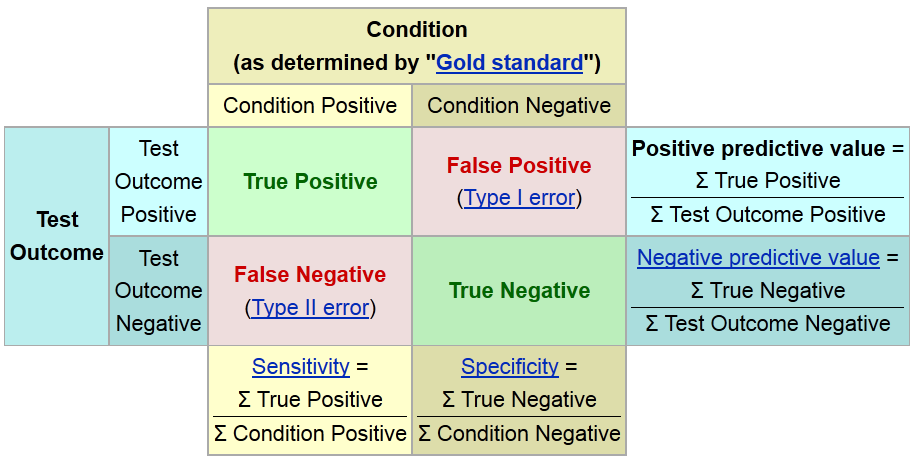
\includegraphics[width=0.75\textwidth]{../Images/Sensitivity_Specificity_Diagram.png}\\
  \caption{Relationship between sensitivity, specificity, positive predictive value and negative predictive value. (From: Wikipedia)}\label{fig:sens_spec_diagram}
\end{figure}

\begin{itemize}
  \item \textbf{Sensitivity} = proportion of positives that are correctly identified by a test = probability of a positive test, given the patient is ill.
  \item \textbf{Specificity} = proportion of negatives that are correctly identified by a test = probability of a negative test, given that patient is well.
  \item \textbf{Positive predictive value} = proportion of patients with positive test results who are correctly diagnosed.
  \item \textbf{Negative predictive value} = proportion of patients with negative test results who are correctly diagnosed.
\end{itemize}

While sensitivity and specificity are independent of prevalence, they do not tell us what portion of patients with abnormal test results are truly abnormal. This information is provided by the positive/negative predictive value. However, as Fig. \ref{fig:prevalence} indicates, these values are affected by the \emph{prevalence} \index{general}{prevalence} of the disease. In other words, we need to know the prevalence of the disease as well as the PPV/NPV of a test to provide a sensible interpretation of the test results.

\begin{figure}[ht]
  \centering
  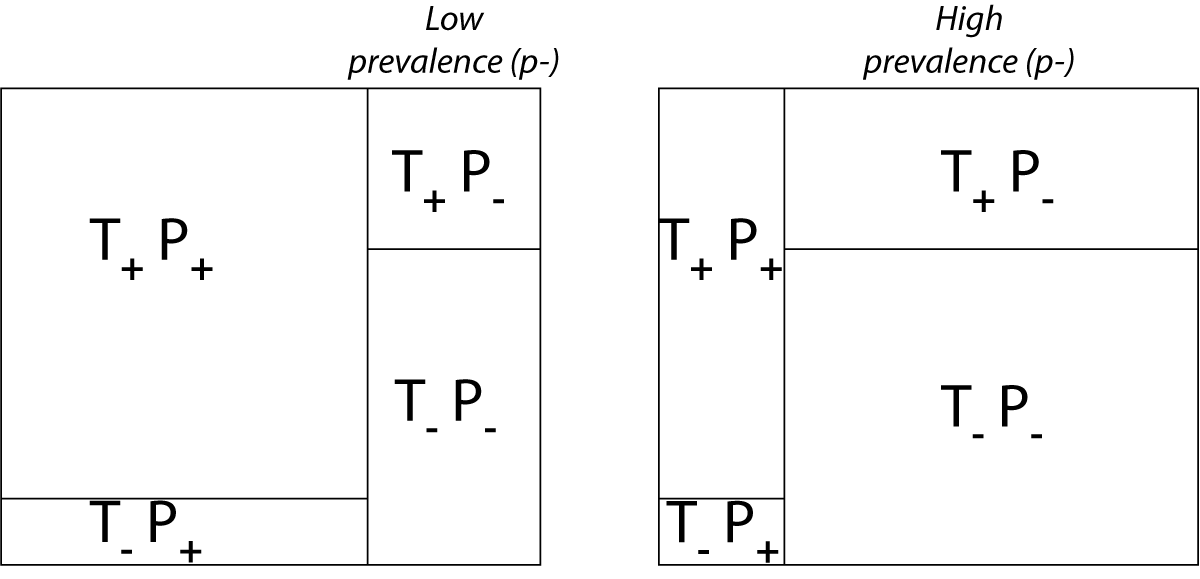
\includegraphics[width=0.75\textwidth]{../Images/Sensitivity_Specificity.png}\\
  \caption{Effect of prevalence on PPV and NPV. "T" stands for "test", and "P" for "patient". (For comparison with below: T+P+ = TP, T-P- = TN, T+P- = FP, and T-P+ = FN)} \label{fig:prevalence}
\end{figure}

Figure \ref{fig:sens_spec_example} gives a worked example:

\begin{figure}[ht]
  \centering
  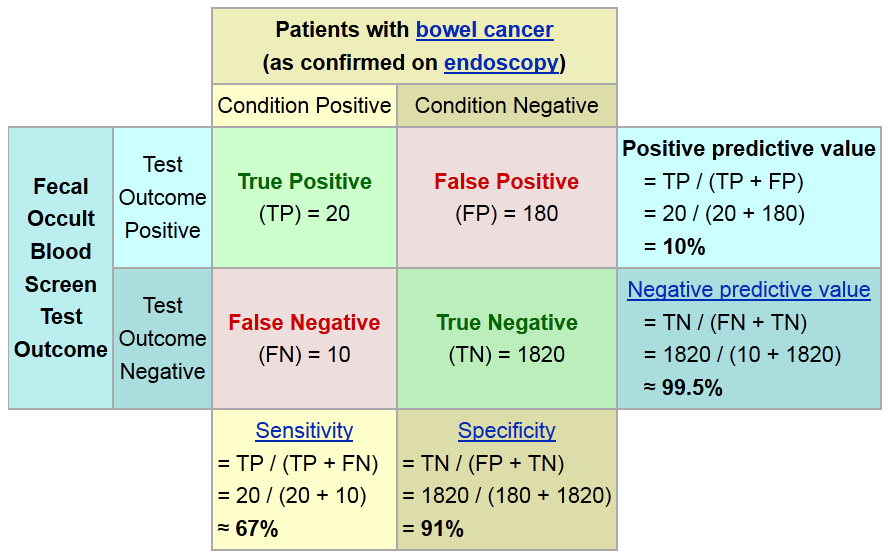
\includegraphics[width=0.75\textwidth]{../Images/Sensitivity_Specificity_Example.png}\\
  \caption{Worked example. (From: Wikipedia)}\label{fig:sens_spec_example}
\end{figure}

\paragraph{Related calculations}

\begin{itemize}
  \item False positive rate ($\alpha$) = type I error = $1 - specificity$ = $\frac{FP}{FP + TN}$ = $\frac{180}{180+1820}$ = 9\%
  \item False negative rate ($\beta$) = type II error = $1 - sensitivity$ = $\frac{FN}{TP + FN}$ = $\frac{10}{20+10}$ = 33\%
  \item Power = sensitivity = $1−\beta$
  \item Likelihood ratio positive = $\frac{sensitivity}{1−specificity}$ = $\frac{66.67\%}{1−91\%}$ = 7.4
  \item Likelihood ratio negative = $\frac{1−sensitivity}{specificity}$ = $\frac{1−66.67\%}{91\%}$ = 0.37
\end{itemize}

Hence with large numbers of false positives and few false negatives, a positive FOB screen test is in itself poor at confirming cancer (PPV = 10\%) and further investigations must be undertaken; it did, however, correctly identify 66.7\% of all cancers (the sensitivity). However as a screening test, a negative result is very good at reassuring that a patient does not have cancer (NPV = 99.5\%) and at this initial screen correctly identifies 91\% of those who do not have cancer (the specificity).

\section{ROC Curve}\index{general}{ROC curve}

Closely related to \emph{Sensitivity} and \emph{Specificity} is the \emph{receiver operating characteristic (ROC)} curve. This is a graph displaying the relationship between the true positive rate (on the vertical axis) and the false positive rate (on the horizontal axis). The technique comes from the field of engineering, where it was developed to find the predictor which best discriminates between two given distributions. In the ROC-curve (Figure \ref{fig:ROC}) this point is given by the value with the largest distance to the diagonal.

\begin{figure}[ht]
  \centering
  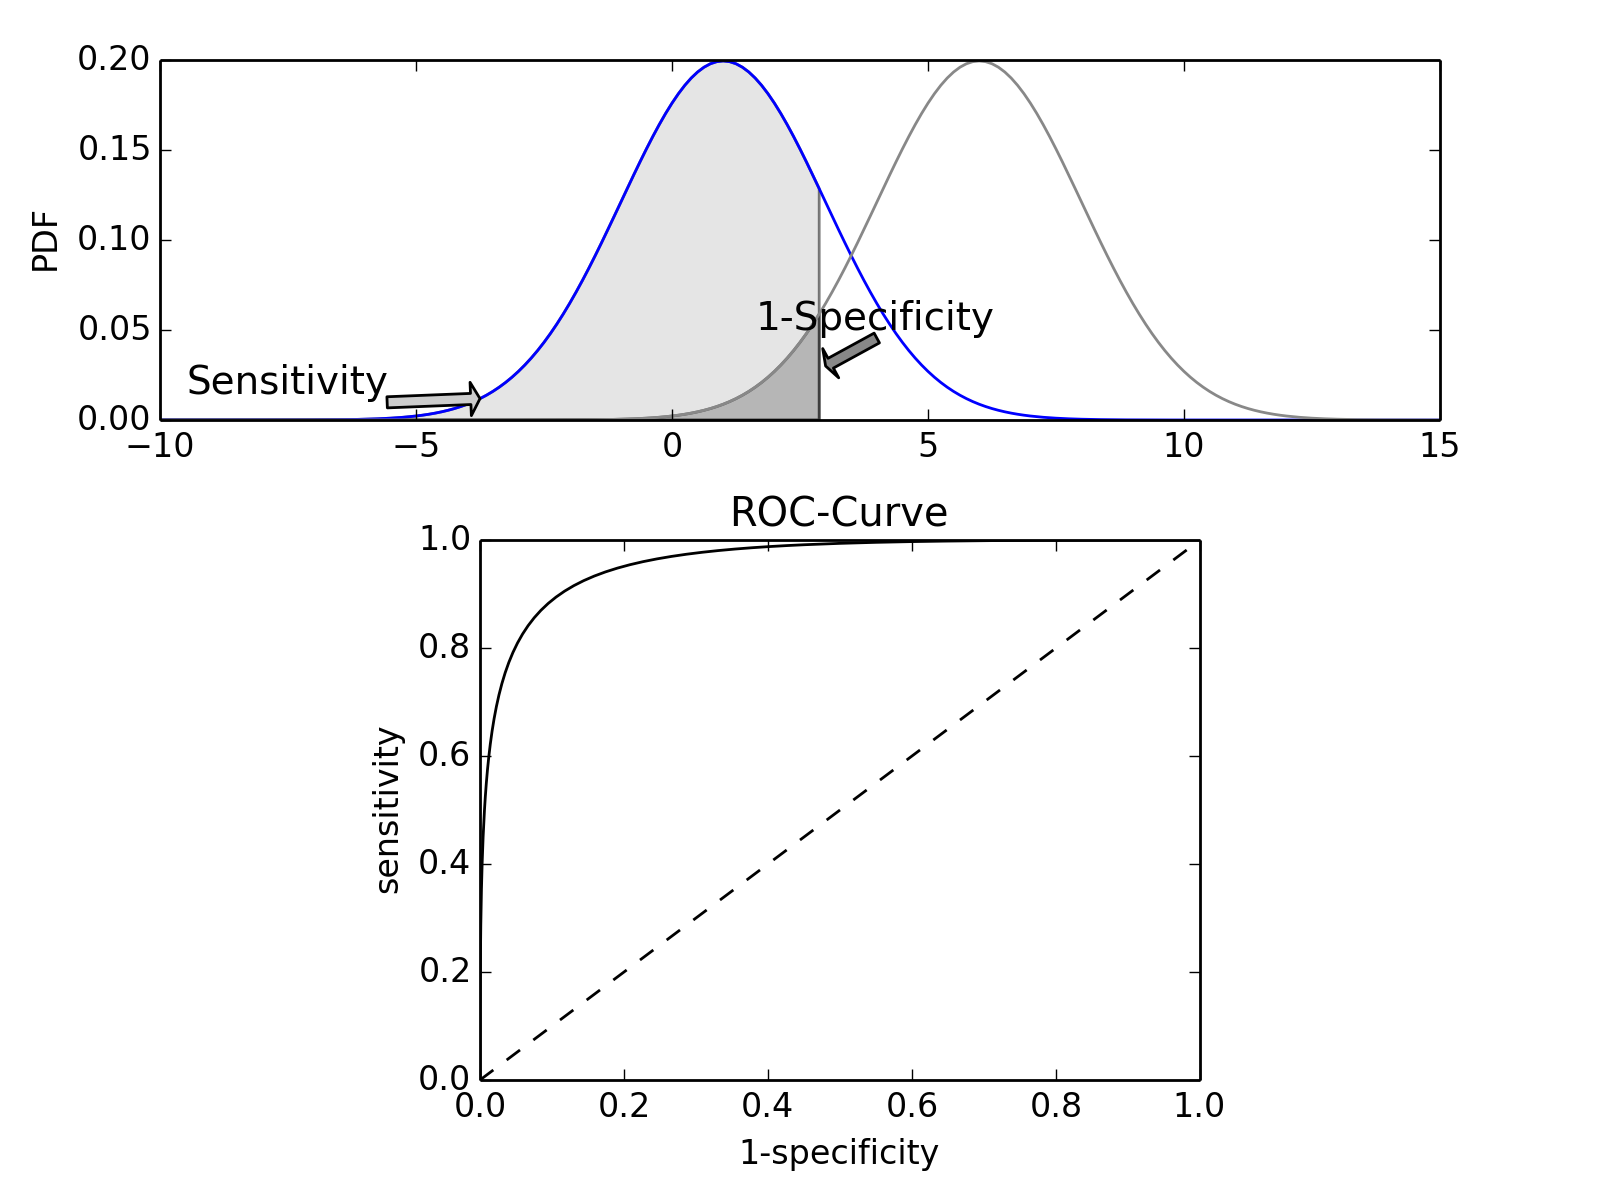
\includegraphics[width=0.75\textwidth]{../Images/ROC.png}\\
  \caption{Top: Probability density functions for two distributions. Bottom: corresponding \emph{ROC-curve}.}\label{fig:ROC}
\end{figure}

\section{Common Statistical Tests for Comparing Groups of Independent and Paired Samples}

Table \ref{table:tests} gives an overview of the most common statistical tests for different combinations of data.
\begin{table}
  \centering
  \footnotesize{
  \begin{tabular}{ | p{5cm} || p{5cm} | p{5cm} | }
     \hline
     No. of Groups Compared  & \textbf{Independent Samples} & \textbf{Paired Samples} \\ \hline
     \textbf{Groups of Nominal Data} & & \\ \hline
     2 or more & Fisher's exact test or Chi-Square test & McNemar's test \\ \hline
     \textbf{Groups of Ordinal Data} & & \\ \hline
     2 & Mann-Whitney U test & Wilcoxon signed rank test \\ \hline
     3 or more & Kruskal-Wallis test & Friedman test \\ \hline
     \textbf{Groups of Continuous Data} & & \\ \hline
     2 & Student's t-test or Mann-Whitney test & Paired t-test or Wilcoxon signed-rank test \\ \hline
     3 or more & ANOVA or Kruskal-Wallis test & Repeated Measures ANOVA or Friedman test \\ \hline

  \end{tabular}
  }

  \caption{Typical tests for statistical problems.}\label{table:tests}
\end{table}


\chapter{Test of Means of Continuous Data}

\section{Distribution of a Sample Mean}

\subsection{One sample t-test for a mean value} \index{general}{test! t-test, one sample}

To check the mean value of normally distributed data against a reference value, we typically use the \emph{one sample t-test}, which is based on the \emph{t-distribution}.

If we knew the mean and the standard deviation of a normally distributed population, we could calculate the corresponding standard error, and use values from the normal distribution to determine how likely it is to find a certain mean value, given the population mean and standard deviation. However, in practice we have to \emph{estimate} the mean and standard deviation from the sample, and the t-distribution for the mean slightly deviates from a normal distribution.

\subsubsection{Example}

Let us look at a specific example: we take 100 normally distributed data, with a mean of 7 and with a standard deviation of 3.
What is the chance of finding a mean value at a distance of 0.5 or more from the mean? \emph{Answer: The probability from the t-test in the example is 0.057, and from the normal distribution 0.054}

Since it is very important to understand the basic principles of how we arrive at the t-statistic and the corresponding p-value for this test, let me illustrate the underlying statistics by going step-by-step through the analysis:

\begin{figure}[h]
  \centering
  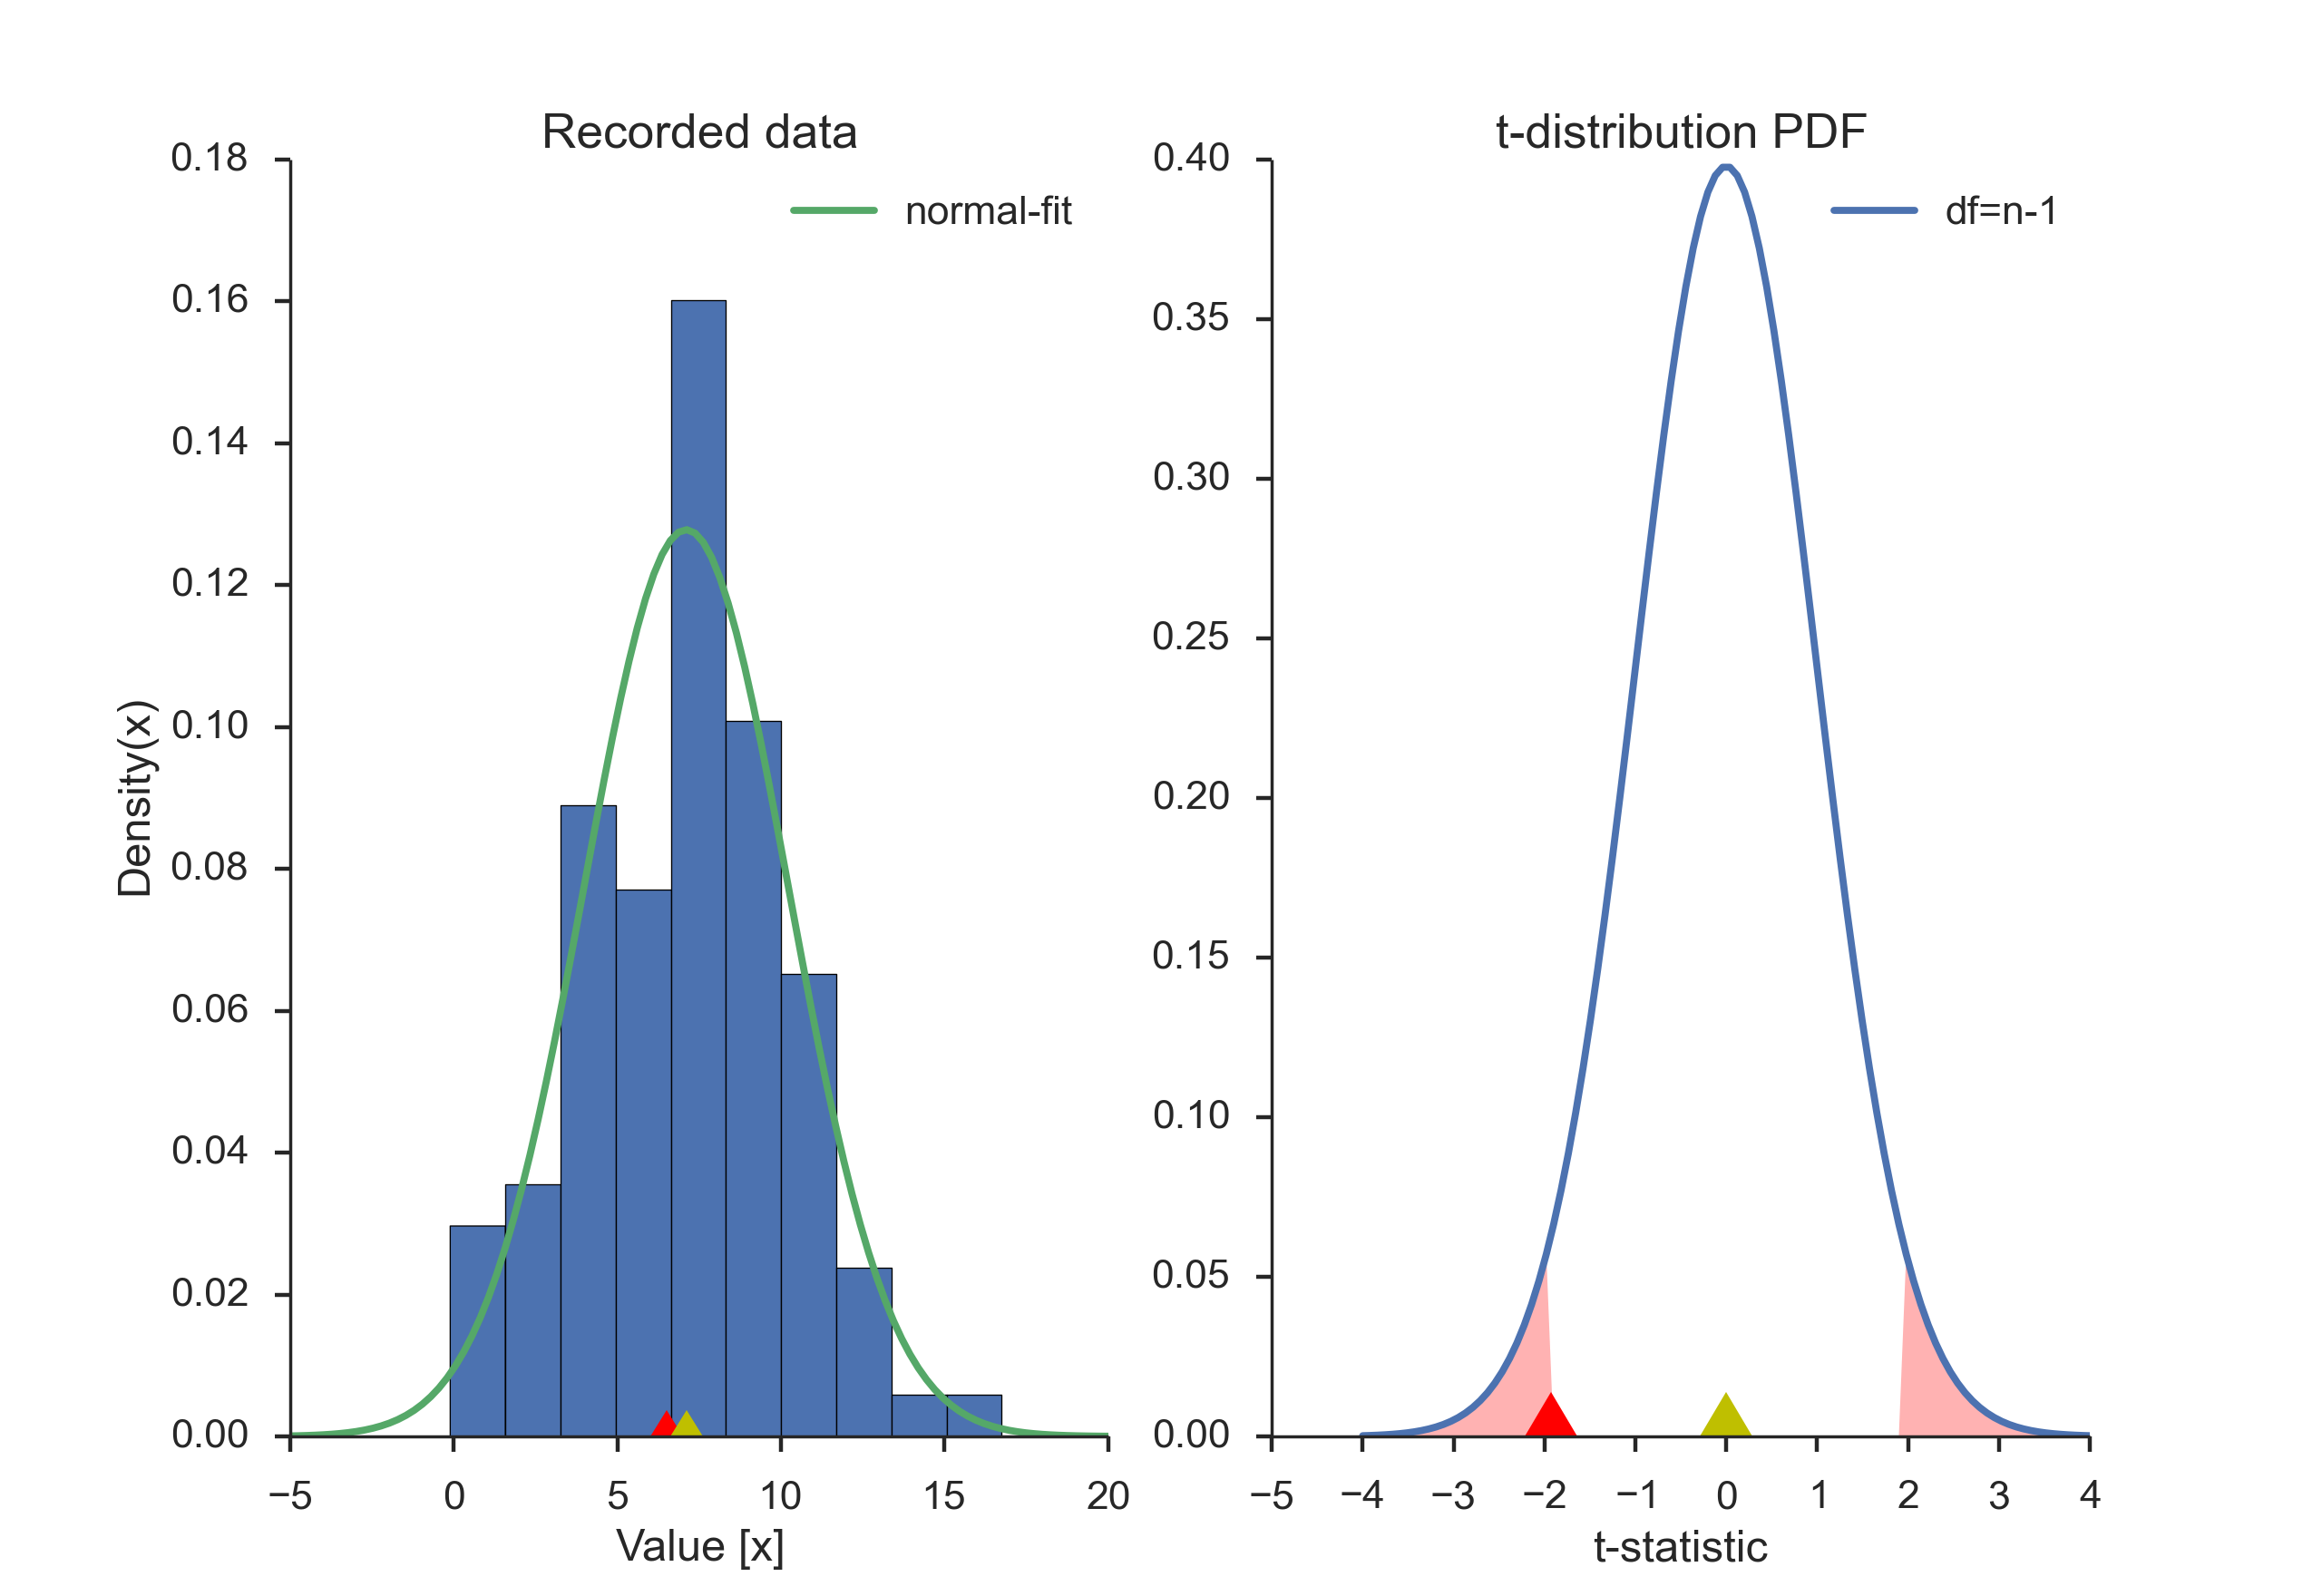
\includegraphics[width=0.75\textwidth]{../Images/ttestExplained.png}\\
  \caption{Left: Frequency histogram of the sample data, together with a normal fit. The sample mean, which is very close to the population mean, is indicated with a yellow triangle; the value to be checked with a red triangle. Right: t-distribution for n-1 degrees of freedom. At the bottom the normalized value of sample mean (yellow triangle) and value to be checked (red triangle). The red shaded area corresponds to the p-value.}\label{fig:ttestExplained}
\end{figure}

\begin{itemize}
  \item We have a population, with a mean value of 7 and a standard deviation of 3.
  \item From that population an observer takes 100 random samples. The sample mean is 7.10, close to but different from the real mean. The sample standard deviation is 3.12, and the standard error of the mean 0.312. This gives the observer an idea about the variability of the population.
  \item The observer knows that the distribution of the real mean follows a t-distribution, and that the \emph{standard error of the mean} characterizes the width of that distribution.
  \item How likely it is that the real mean has a value of $x_0$ (e.g. 6.5, indicated by the red triangle in Fig. \ref{fig:ttestExplained}, left)? To find that out, this value has to be transformed, by subtracting the sample mean, and dividing by the standard error. (Fig. \ref{fig:ttestExplained}, right). This provides the \emph{t-statistic} for this test (-1.93).
  \item The corresponding \emph{p-value}, which tells us how likely it is that the real mean has a value of 6.5 or more extreme relative to the sample mean, is given by the red shaded area under the curve-wings: \emph{2*CDF(t-statistic) = 0.057}, which means that the difference to 6.5 is just not significant. (The factor "2" comes from the fact that we have to check in both tails.)
\end{itemize}

\PyImg "oneSample.py" (p \pageref{py:oneSample}): Sample analysis for one group of continuous data.
\index{python}{oneSample}

%To illustrate the ideas behind the use of distribution functions, let us go step-by-step through the analysis of the following problem:
%Being 50 years old, 175 cm tall, and moderately active, my daily nutritional requirement is 2460 cal/day. On 10 subsequent days, I have carefully listed my food intake, and obtained the following numbers of calories for each day: [2784, 2632, 2771, 2495, 2435, 2513, 2633, 2737, 2687, 2647]. My question now: is this too much - do I have to cut back on my chocolate??
%
%\begin{itemize}
%  \item Find the mean and standard deviation of the best-fit normal distribution (mean = 2633.4, std = 113.3).
%  \item Calculate the CDF at the interesting value (2460 cal/day) (CDF(2460) = 0.06).
%  \item Interpret the result (\emph{"not significant"}).
%\end{itemize}
%
%\begin{figure}[h]
%  \centering
%  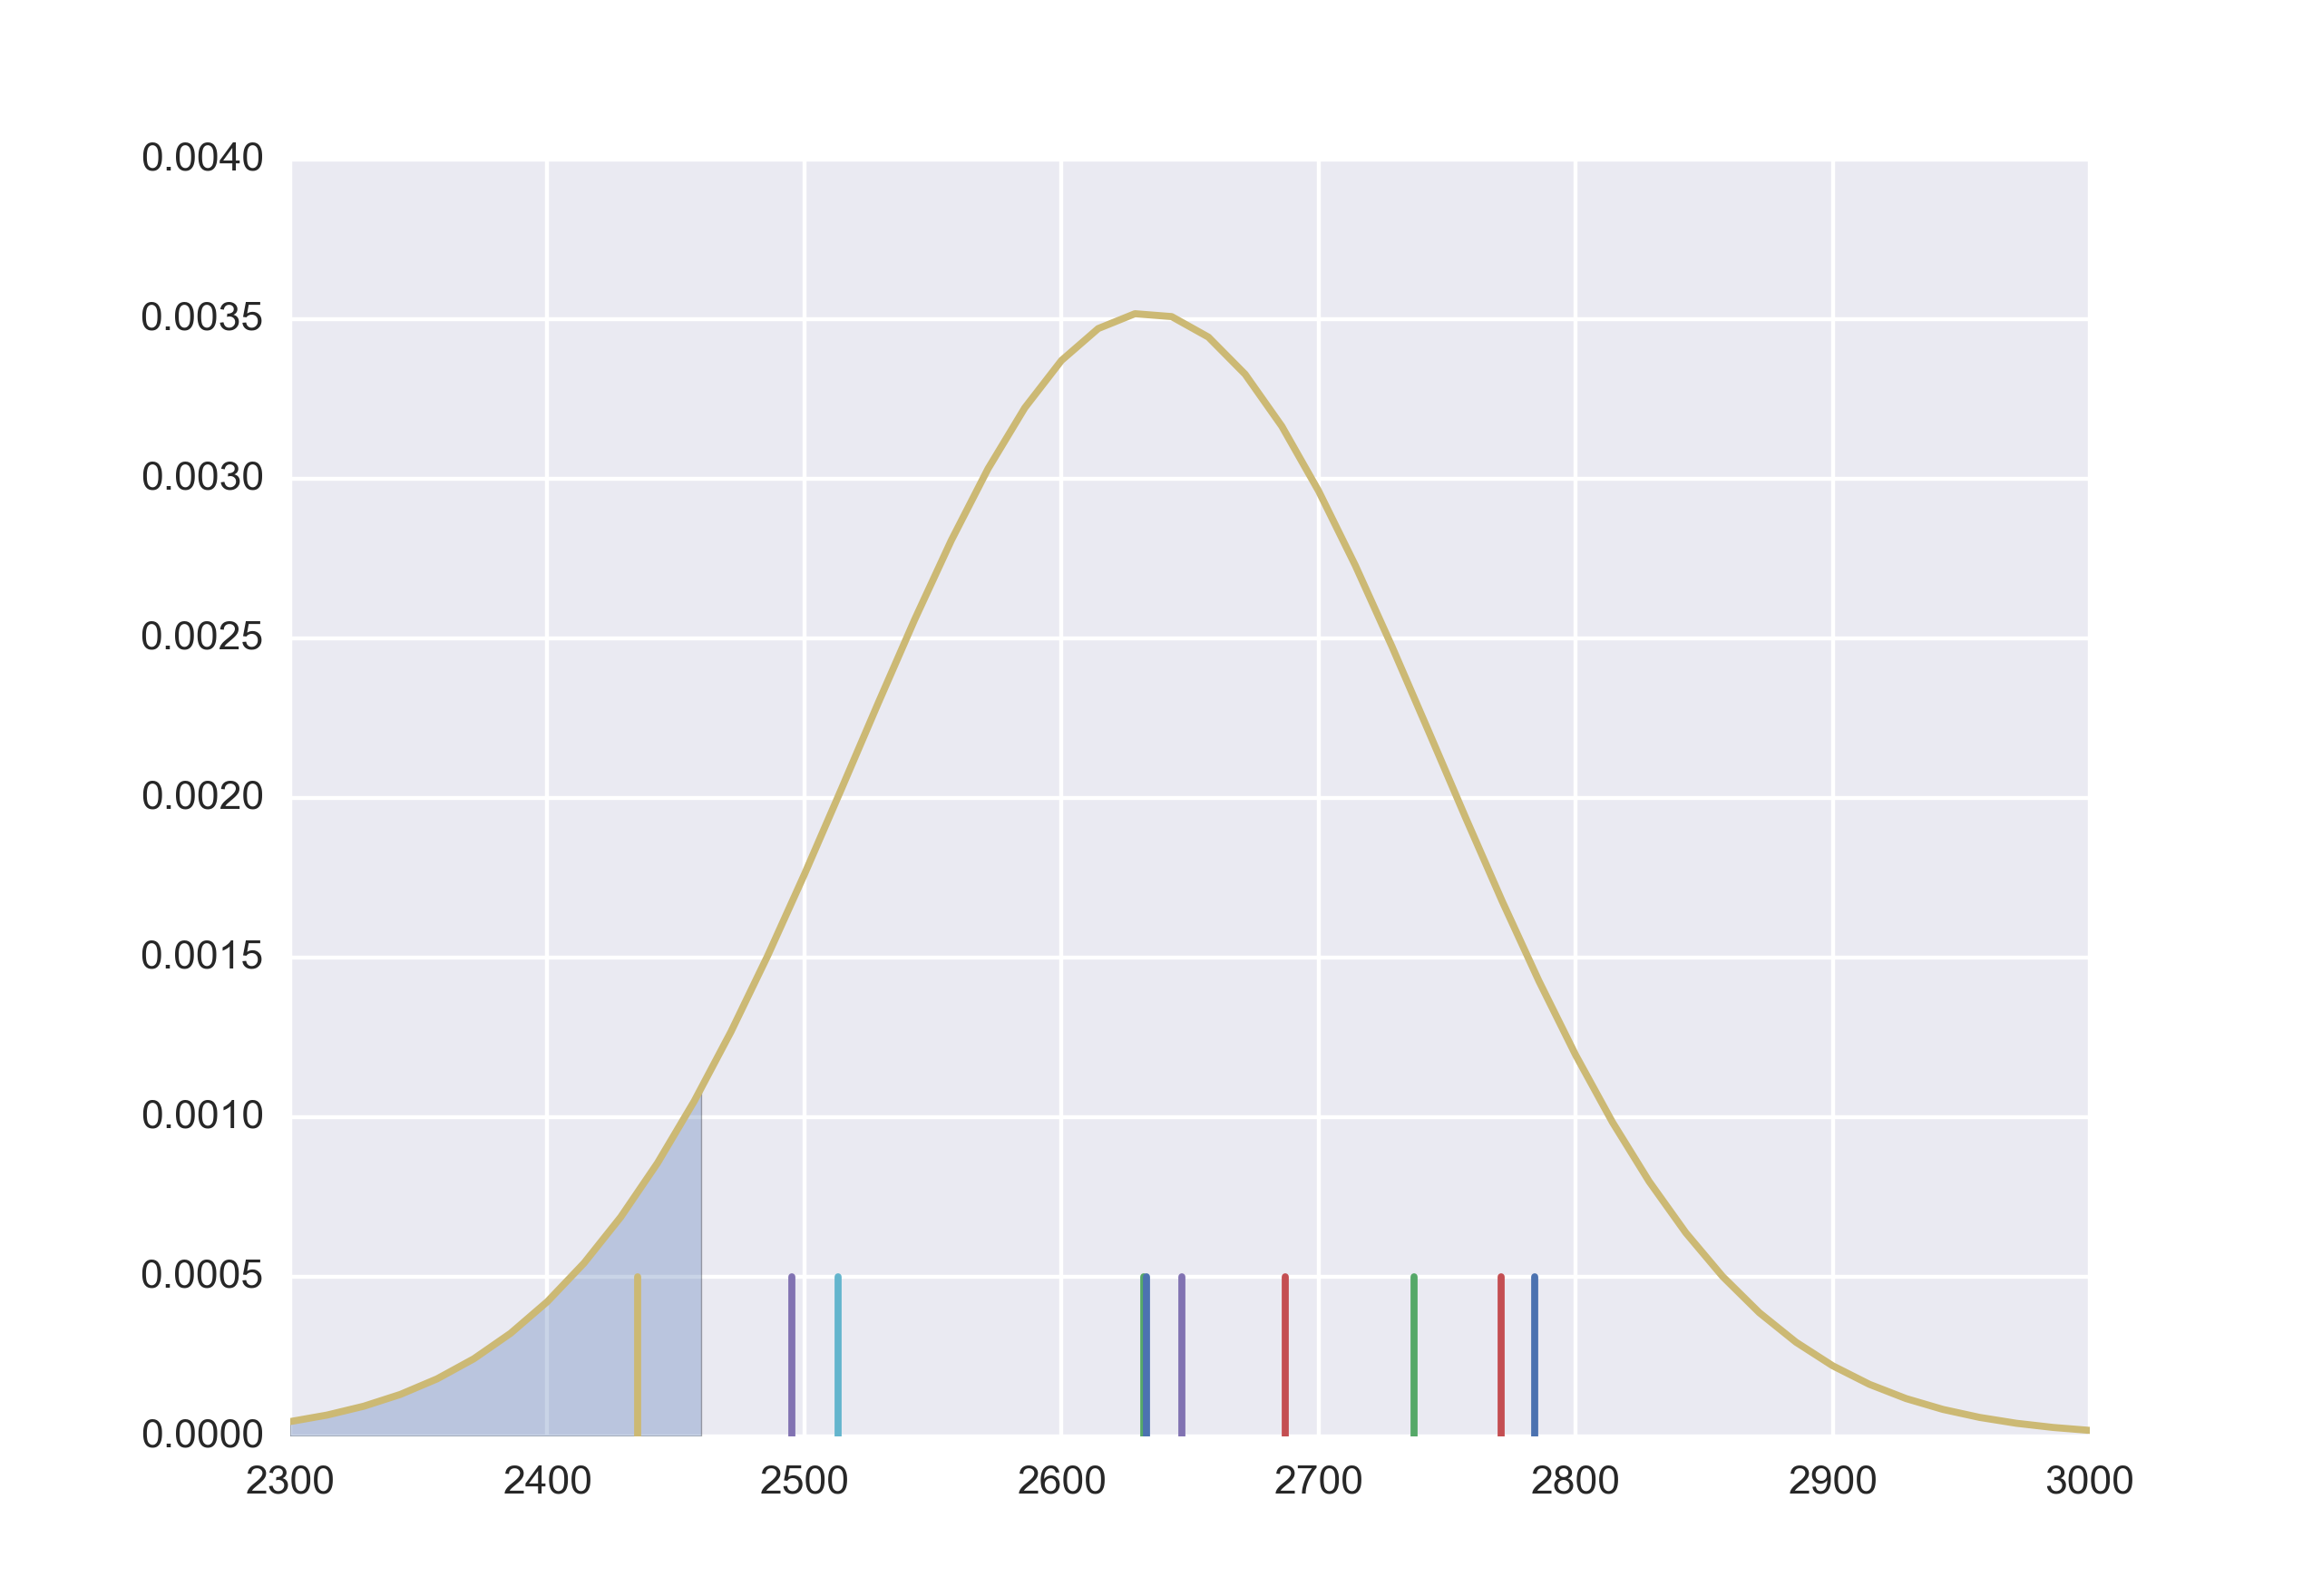
\includegraphics[width=0.85\textwidth]{../Images/pdf_checkMean.png}\\
%  \caption{Check if the mean of the fitted curve is significantly different from the value to be checked.}\label{fig:pdf_checkValue}
%\end{figure}


\subsection{Wilcoxon signed rank sum test}\index{general}{test!Wilcoxon signed rank sum}

If our data are not normally distributed, we cannot use the t-test (although this test is fairly robust against deviations from normality). Instead, we must use a \emph{non-parametric} test on the mean value. We can do this by performing a \emph{Wilcoxon signed rank sum test}.
 \footnote{Python Example: scipy.stats.wilcoxon, in "univariate.py"}
\footnote{The following description and example has been taken from \cite{altman99}, Table 9.2}
This method has three steps:

\begin{enumerate}
  \item Calculate the difference between each observation and the value of interest.
  \item Ignoring the signs of the differences, rank them in order of magnitude.
  \item Calculate the sum of the ranks of all the negative (or positive) ranks, corresponding to the observations below (or above) the chosen hypothetical value.
\end{enumerate}

In Table \ref{tab:wilcoxon} you see an example, where the significance to a deviation from the value of 7725 is tested. The rank sum of the negative values gives $3+5=8$, and can be looked up in the corresponding tables to be significant. In practice, your computer program will nowadays do this for you. This example also shows another feature of rank evaluations: tied values (here $7515$) get accorded their mean rank (here $1.5$).

\begin{table}
  \centering
  \begin{tabular}{l p{2cm} p{2cm} p{2cm}}
     \hline
     Subject & Daily energy intake (kJ) & Difference from 7725 kJ & Ranks of differences \\
     1 & 5260 & 2465 & 11 \\
     2 & 5470 & 2255 & 10 \\
     3 & 5640 & 2085 & 9 \\
     4 & 6180 & 1545 & 8 \\
     5 & 6390 & 1335 & 7 \\
     6 & 6515 & 1210 & 6 \\
     7 & 6805 & 920 & 4 \\
     8 & 7515 & 210 & 1.5 \\
     9 & 7515 & 210 & 1.5 \\
     10 & 8230 & -505 & 3 \\
     11 & 8770 & -1045 & 5 \\
     \hline
   \end{tabular}
  \caption{Daily energy intake of 11 healthy women with rank order of differences (ignoring their signs) from the recommended intake of 7725 kJ.}\label{tab:wilcoxon}
\end{table}


\section{Comparison of Two Groups} \index{general}{test! t-test, paired}

When you compare two groups with each other, we have to distinguish between two cases. In the first case, we compare two values recorded from the same subject at two specific times. For example, we measure the size of students when they enter primary school and after their first year, and check if they have been growing. Since we are only interested in the \emph{difference} between the first and the second measurement, this test is called \emph{paired t-test}, and is essentially equivalent to a one-sample t-test for the mean difference.

The second test is if we compare two independent groups. For example, we can compare the effect of a two medications given to two different groups of patients, and compare how the two groups respond. This is called an \emph{unpaired t-test}, or \emph{t-test for two independent groups}.

If we have two independent samples the variance of the difference between their means is the \emph{sum} of the separate variances, so the standard error of the difference in means is the square root of the sum of the separate variances:

\begin{align*}
   se({{\bar x}_1} - {{\bar x}_2}) &= \sqrt {\operatorname{var} ({{\bar x}_1}) + \operatorname{var} ({{\bar x}_2})}  \\
   &= \sqrt {{{\left\{ {se({{\bar x}_1})} \right\}}^2} + {{\left\{ {se({{\bar x}_2})} \right\}}^2}}  \\
   &= \sqrt {\frac{{s_1^2}}{{{n_1}}} + \frac{{s_2^2}}{{{n_2}}}}  \\
\end{align*}

where $\bar{x}_i$ is the mean of the i-th sample, and \emph{se} indicates the \emph{standard error}.

\subsection{Non-parametric Comparison of Two Groups: Mann-Whitney Test} \index{general}{test!Mann-Whitney}\label{test:Mann-Whitney}

If the measurement values from the two groups are not normally distributed we have to resort to a non-parametric test. The most common test for that is the \emph{Mann-Whitney(-Wilcoxon) test}. Watch out, because this test is sometimes also referred to as \emph{Wilcoxon rank-sum test}. This is different than the \emph{Wilcoxon signed rank sum test}!

\PyImg "twoSample.py" (p \pageref{py:twoSample}): Comparison of two groups, paired and unpaired.
\index{python}{twoSample}

\subsection{Statistical Tests vs Statistical Modeling}

With the advent of cheap computing power, statistical modeling has been a booming field. This has also affected classical statistical analysis, as most problems can be viewed from two perspectives: you can either make a statistical hypothesis, and verify or falsify that hypothesis; or you can make a statistical model, and analyse the significance of the model parameters.

Let me use a classical t-test as an example.

\subsubsection{Classical t-test}

Let us take performance measurements from a racing team, on two different occasions. During Race\_1, the members of the team achieve a score of [ 79.,  100.,   93.,   75.,   84.,  107.,   66.,   86.,  103.,
         81.,   83.,   89.,  105.,   84.,   86.,   86.,  112.,  112.,
        100.,   94.], and during Race\_2 [  92.,  100.,   76.,   97.,   72.,   79.,   94.,   71.,   84.,
         76.,   82.,   57.,   67.,   78.,   94.,   83.,   85.,   92.,
         76.,   88.].

These numbers can be generated, and a t-test comparing the two groups can be done, with the following Python commands:

\begin{lstlisting}
    from scipy import stats
    random.seed(123)
    race_1 = np.round(randn(20)*10+90)
    race_2 = np.round(randn(20)*10+85)
    stats.ttest_rel(race_1, race_2)
\end{lstlisting}

\subsubsection{Statistical Modeling}

\begin{lstlisting}
    import pandas as pd
    import statsmodels.formula.api as sm
    df = pd.DataFrame({'Race1': race_1, 'Race2':race_2})
    result = sm.ols(formula='I(Race2-Race1) ~ 1', data=df).fit()
    print result.summary()
\end{lstlisting}


\section{Comparison of More Groups}

\subsection{Analysis of Variance - ANOVA} \label{sec:anova} \index{general}{ANOVA} \index{general}{test!ANOVA}

The idea behind the \emph{ANalysis Of VAriance (ANOVA)} is to divide the variance into the variance \emph{between} groups, and that \emph{within} groups, and see if those distributions match the null hypothesis that all groups come from the same distribution. The variables that distinguish the different groups are often called \emph{factors}.

(By comparison, t-tests look at the mean values of two groups, and check if those are consistent with the assumption that the two groups come from the same distribution.)

For example, if we compare a group with No treatment, another with treatment A, and a third with treatment B, then we perform a \emph{one factor ANOVA}, sometimes also called \emph{one-way ANOVA}, with "treatment" the one analysis factor. If we do the same test with men and with women, then we have a \emph{two-factor} or \emph{two-way ANOVA}, with "gender" and "treatment" as the two treatment factors. Note that with ANOVAs, it is quite important to have exactly the same number of samples in each analysis group!

Because the null hypothesis is that there is no difference between the groups, the test is based on a comparison of the observed variation between the groups (i.e. between their means) with that expected from the observed variability between subjects. The comparison takes the general form of an \emph{F test} to compare variances, but for two groups the t test leads to exactly the same answer.

The one-way ANOVA assumes all the samples are drawn from normally distributed populations with equal variance. To test this assumption, you can use the \emph{Levene test}\index{general}{test!Levene}.

ANOVA uses traditional standardized terminology. The definitional equation
of sample variance is $s^2=\textstyle\frac{1}{n-1}\sum(y_i-\bar{y})^2$,
where
the divisor is called the degrees of freedom (DF), the summation is called
the sum of squares (SS), the result is called the mean square (MS) and the
squared terms are deviations from the sample mean. ANOVA estimates 3 sample
variances: a total variance based on all the observation deviations from the
grand mean, an error variance based on all the observation deviations from
their appropriate treatment means and a treatment variance. The treatment
variance is based on the deviations of treatment means from the grand mean,
the result being multiplied by the number of observations in each treatment
to account for the difference between the variance of observations and the
variance of means. If the null hypothesis is true, all three variance
estimates are equal (within sampling error).

The fundamental technique is a partitioning of the total sum of squares SS
into components related to the effects used in the model. For example, the
model for a simplified ANOVA with one type of treatment at different levels.

\begin{equation}
  SS_\text{Total} = SS_\text{Error} + SS_\text{Treatments}
\end{equation}


The number of degrees of freedom DF can be partitioned in a similar way: one
of these components (that for error) specifies a chi-squared distribution
which describes the associated sum of squares, while the same is true for
"treatments" if there is no treatment effect.

\begin{equation}
  DF_\text{Total} = DF_\text{Error} + DF_\text{Treatments}
\end{equation}


\subsubsection{Example: one-way ANOVA}
As an example, let us take the red cell folate levels ($\mu g/l$) in three groups of cardiac bypass patients given different levels of nitrous oxide ventilation (Amess et al, 1978), described in the Python code example
below. I first show the result of this ANOVA test, and then explain the steps
to get there.

\begin{verbatim}
                DF    SS          MS     F    p(>F)
  C(treatment)   2  15515.76  7757.88  3.71  0.043
  Residual      19  39716.09  2090.32   NaN    NaN
\end{verbatim}

\begin{itemize}
  \item First the "Sums of squares (SS)" are calculated. Here the SS between treatments is 15515.88, and the SS of the residuals is 39716.09 . The total SS is the sum of these two values.
  \item The mean squares (MS) is the SS divided by the corresponding degrees of freedom (DF).
  \item The \emph{F-test}\index{general}{test!F-test} or \emph{variance ratio test}\index{general}{test!variance ratio} is used for comparing the factors of the total deviation. The F-value is the larger mean squares value divided by the smaller value. (If we only have two groups, the F-value is the square of the corresponding t-value. See \ref{py:anovaOneway}).

      \begin{eqnarray}
        F &=& \frac{\text{variance between treatments}}{\text{variance within treatments}} \\
        F &=& \frac{MS_\text{Treatments}}{MS_\text{Error}} = {{SS_\text{Treatments} / (n_{groups}-1)} \over {SS_\text{Error} / (n_{total}-n_{groups})}}
      \end{eqnarray}

  \item Under the null hypothesis that two normally distributed populations have equal variances we expect the ratio of the two sample variances to have an \emph{F Distribution} (see section \ref{sec:ContinuousDistributions}). From the F-value, we can look up the corresponding p-value.
\end{itemize}

\PyImg "anovaOneway.py" (p \pageref{py:anovaOneway}): different aspects of one-way ANOVAs.
\index{python}{anovaOneway}

\subsection{Multiple Comparisons}\index{general}{Multiple Comparisons}

The Null hypothesis in a one-way ANOVA is that the means of all the samples are the same. So if a one-way ANOVA yields a significant result, we only know that they are \emph{not} the same.

However, often we are not just interested in the joint hypothesis if all samples are the same, but we would also like to know for which pairs of samples the hypothesis of equal values is rejected. In this case we conduct several tests at the same time, one test for each pair of samples. (Typically, this is done with $t-tests$.)

This results, as a consequence, in a \emph{multiple testing problem}:
since we perform multiple comparison tests, we should compensate for the risk of getting a significant result, even if our null hypothesis is true. This can be cone by correcting the p-values to account for this. We have a number of options to do so:

\begin{itemize}
  \item Tukey HSD
  \item Bonferroni correction
  \item Holms correction
  \item ... and others ...
\end{itemize}


\subsubsection{Tukey's Test}\index{general}{test!Tukey's}

\emph{Tukey's test}, sometimes also referred to as the \emph{Tukey Honest Significant Difference (HSD) method }, controls for the Type I error rate across multiple comparisons and is generally considered an acceptable technique. It is based on a formula very similar to that of the t-test. In fact, Tukey's test is essentially a t-test, except that it corrects for multiple comparisons.

The formula for Tukey's test is:

\begin{equation}
    q_s = \frac{Y_A - Y_B}{SE}
\end{equation}

where $Y_A$ is the larger of the two means being compared, $Y_B$ is the smaller of the two means being compared, and $SE$ is the standard error of the data in question. This $q_s$ value can then be compared to a q value from the \emph{studentized range distribution}, which takes into account the multiple comparisons. If the q value is larger than the critical value obtained from the distribution, the two means are said to be significantly different.
Note that the studentized range statistic is the same as the t-statistic except for a scaling factor (np.sqrt(2)).

\PyImg "multipleTesting.py" (p \pageref{py:multipleTesting}): this script provides an example where three treatments are compared.
\index{python}{multipleTesting}

\begin{figure}[h]
  \centering
  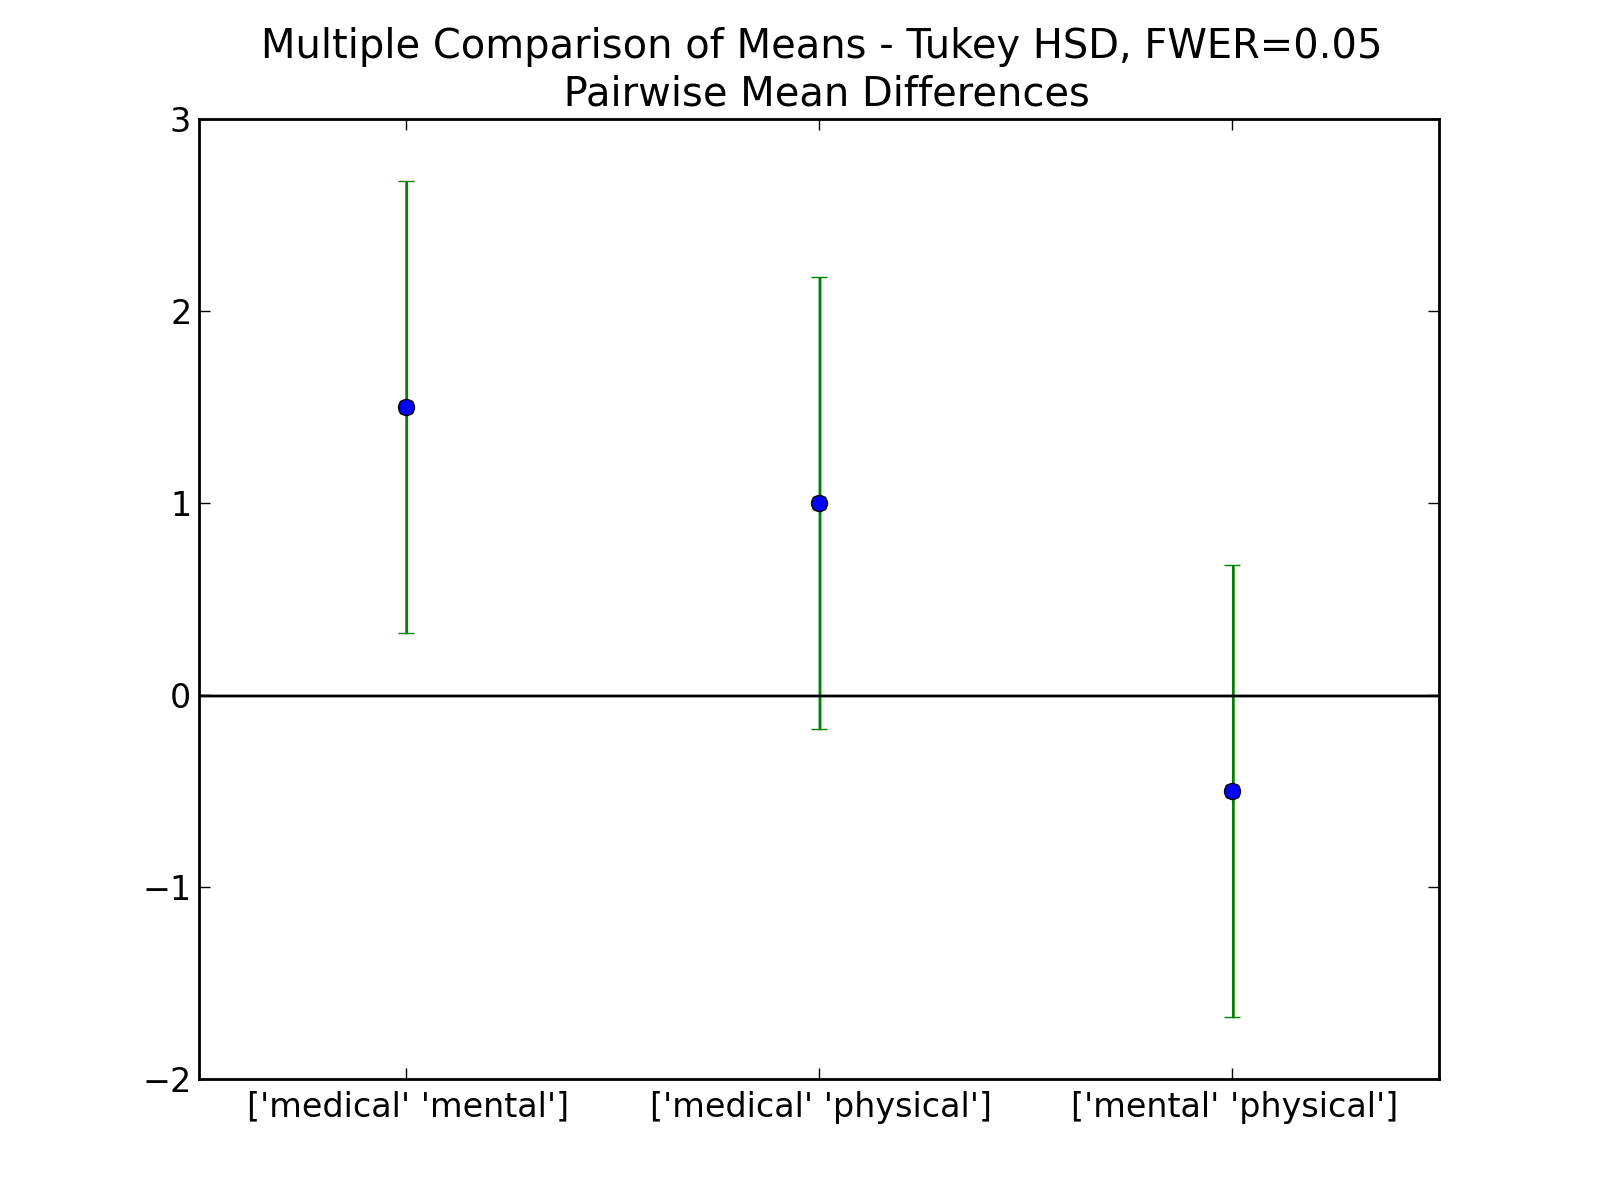
\includegraphics[width=0.5\textwidth]{../Images/MultComp.png}\\
  \caption{Comparing the means of multiple groups - here three different treatment options.}
\end{figure}

\subsubsection{Bonferroni correction}\index{general}{Bonferroni correction}

Tukey's studentized range test (HSD) is a test specific to the comparison of all pairs of k independent samples. Instead we can run t-tests on all pairs, calculate the p-values and apply one of the p-value corrections for multiple testing problems. The simplest - and at the same time quite conservative - approach is to divide the required p-value by the number of tests that we do (\emph{Bonferroni correction}). For example, if you perform 4 comparisons, you check for significance not at $p=0.05$, but at $p=0.0125$.

While multiple testing is not yet included in Python standardly, you can get a number of multiple-testing corrections done with the statsmodels package:

\begin{lstlisting}
  In[7]: from statsmodels.sandbox.stats.multicomp import multipletests
  In[8]: multipletests([.05, 0.3, 0.01], method='bonferroni')
Out[8]:
  (array([False, False,  True], dtype=bool),
  array([ 0.15,  0.9 ,  0.03]),
  0.016952427508441503,
  0.016666666666666666)
\end{lstlisting}

\subsubsection{Holms correction}\index{general}{Holms correction}

The Holm adjustment sequentially compares the lowest p-value with a Type I error rate that is reduced for each consecutive test. For example, if you have three groups (and thus three comparisons), this means that the first p-value is tested at the .05/3 level (.017), the second at the .05/2 level (.025), and third at the .05/1 level (.05). This method is generally considered superior to the Bonferroni adjustment.

\subsection{Kruskal-Wallis test}\index{general}{test!Kruskal-Wallis}\label{test:Kruskal-Wallis}

When we compare two groups to each other, we use the \emph{t-test} when the data are normally distributed and the non-parametric \emph{Mann-Whitney test} otherwise. For three or more groups, the test for normally distributed data is the \emph{ANOVA-test}; for not-normally distributed data, the corresponding test is the \emph{Kruskal-Wallis test}. When the null hypothesis is true the test statistic for the Kruskal-Wallis test follows the \emph{Chi squared distribution}.

\PyImg "KruskalWallis.py" (p \pageref{py:KruskalWallis}): Example of a Kruskal-Wallis test (for not normally distributed data).
\index{python}{KruskalWallis}

\section{Exercises}

\subsection{One or Two Groups}

\begin{enumerate}
  \item \textbf{Paired T-Test} and \textbf{Wilcoxon signed rank sum test}

The daily energy intake from 11 healthy women is [5260., 5470., 5640., 6180., 6390., 6515., 6805., 7515., 7515., 8230., 8770.] kJ.

    Is this value significantly different from the recommended value of 7725?
    (Correct answer: yes, $p_{ttest}=0.018$, and $p_{Wilcoxon}=0.026$)

  \item \textbf{t-test of independent samples}

In a clinic, 15 lazy patients weight [76., 101., 66., 72., 88., 82., 79., 73., 76., 85., 75., 64., 76., 81., 86.] kg, and 15 sporty patients weigh [ 64., 65., 56., 62., 59., 76., 66., 82., 91., 57., 92., 80., 82., 67., 54.] kg.

    Are the lazy patients significantly heavier?
    (Correct answer: yes, p=0.045)

  \item \textbf{Normality test}

    Are the two datasets normally distributed?
    (Correct answer: yes, they are)

  \item \textbf{Mann-Whitney test}

    Are the lazy patients still heavier, if you check with the Mann-Whitney test?
    (Correct answer: yes, p=0.039)
\end{enumerate}

\subsection{Multiple Groups}

(The following example is taken from the really good, but somewhat advanced book by AJ Dobson: "An Introduction to Generalized Linear Models")

\begin{enumerate}
  \item \textbf{Get the data}

    The file   \emph{https://github.com/thomas-haslwanter/statsintro/blob/master/Data/data\_others/Table 6.6 Plant experiment.xls} contains data from an experiment with plants in three different growing conditions. Get the data into Python.
    Hint: use the module xlrd

  \item \textbf{Perform an ANOVA}

    Are the three groups different?
    (Correct answer: yes, they are.)

  \item \textbf{Multiple Comparisons}

    Using the Tukey test, which of the pairs are different?
    (Correct answer: only TreamtmentA and TreatmentB differ)

  \item \textbf{Kruskal-Wallis}

    Would a non-parametric comparison lead to a different result?
    (Correct answer: no)

\end{enumerate}

\chapter{Tests on Categorical Data }

In a sample of individuals the number falling into a particular group is called the \emph{frequency}, so the analysis of categorical data is the analysis of frequencies. When two or more groups are compared the data are often shown in the form of a \emph{frequency table}, sometimes also called \emph{contingency table}.

\begin{table}
  \centering
  \begin{tabular}{|c|l l l|}
  \hline
  & \emph{Right Handed} & \emph{Left Handed} & \emph{Total} \\
  \hline
  \emph{Males} & 43 & 9 & 52 \\
  \emph{Females} & 44 & 4 & 48 \\
  \emph{Total} & 87 & 13 & 100 \\
  \hline
  \end{tabular}

  \caption{Example of a frequency table}\label{table:frequency}
\end{table}

If you have only one sample group of data, the analysis options are somewhat limited. In contrast, a number of statistical tests exist for the analysis of frequency tables.

\begin{description}
  \item[Chi-square test] This is the most common type. It is a hypothesis test, which checks if the entries in the individual cells all come from the same distribution. In other words, it checks the null hypothesis $H_0$ that the results are independent of the row or column in which they appear. The alternative hypothesis $H_a$ does not specify the type of association, so close attention to the data is required to interpret the information provided by the test.
  \item[Fisher's Exact Test] While the chi-square test is approximate, the \emph{Fisher's Exact Test} is an exact test. As it is computationally much more expensive and intricate than the chi-square test, it was originally used only for small sample numbers. However, in general it is now the more advisable test to use.
  \item[McNemar's Test]  This is a \emph{matched pair test }for 2x2 tables.
  \item[Cochran's Q Test] \index{general}{test!Cochran's Q} Cochran's Q test is an extension to the McNemar's test for related samples that provides a method for testing for differences between three or more \emph{matched/paired} sets of frequencies or proportions. For example, if you have exactly the same samples analyzed by 3 different laboratories, and you want to check if the results are statistically equivalent, you would use this test.
\end{description}


\section{One Proportion}

If you have one sample group of data, you can check if your sample is representative of the standard population. To do so, you have to know the proportion $p$ of the characteristic in the standard population. The occurrence of a characteristic in a group of $n$ people is described by the binomial distribution, with $mean = p*n$. The standard error of samples with this characteristic is given by

\begin{equation}
  se(p) = \sqrt{p(1-p)/n}
\end{equation}

and the corresponding 95\% confidence interval is
\begin{equation*}
  ci = mean \pm se * t_{n,0.95}
\end{equation*}

If your data lie outside this confidence interval, they are \emph{not} representative of the population.

\subsection{Example}

For example, let us look at incidence and mortality for breast cancer, and try to answer the following two questions: among the FH-students, how many occurrences of breast cancer should we expect per year? And how many of the female FH-students will probably die from breast cancer at the end of their life?

We know that:

\begin{itemize}
  \item the FH OOe has about 5'000 students, about half of which are female.
  \item breast cancer hits predominantly women.
  \item the \emph{incidence} of breast cancer in the age group 20-30 is about 10
  \item 3.8\% of all women die of cancer.
\end{itemize}

From these points of information, we can obtain the following parameters for our calculations

\begin{itemize}
  \item n = 2'500
  \item $p_{incidence} = 10 / 100'000$, as \emph{incidence}\index{general}{incidence} is typically defined as the new occurrences of a disease per year per 100'000 people.
  \item $p_{mortality} = 3.8/100$.
\end{itemize}

The 95\% confidence interval for the incidence is -0.7 - 1.2, and for the number of deaths 76 - 114. So we expect that every year most likely none or one of the FH-students will be diagnosed with breast cancer; but between 76 and 114 of the female students will eventually die from this disease.

\section{Frequency Tables} \index{general}{frequency tables}

If your data can be organized in a set of categories, and they are given as \emph{frequencies}, i.e. the total number of samples in each category (not as percentages), the tests described in this section are appropriate for your data analysis.

Many of these tests analyze the \emph{deviation from an expected value}. Since the chi-square distribution characterizes the variability of data (in other words, their deviation from a mean value), many of these tests refer to this distribution, and are accordingly termed \emph{chi-square tests}.

\begin{table}
  \centering
  \begin{tabular}{|c|l l l|}
  \hline
  & \emph{Right Handed} & \emph{Left Handed} & \emph{Total} \\
  \hline
  \emph{Males} & 45.2 & 6.8 & 52 \\
  \emph{Females} & 41.8 & 6.2 & 48 \\
  \emph{Total} & 87 & 13 & 100 \\
  \hline
  \end{tabular}

  \caption{Corresponding expected values for Table \ref{table:frequency}\label{table:expectedValues}}
\end{table}


Assume you have observed absolute frequencies $o_i$ and expected absolute frequencies $e_i$. Under the Null hypothesis all your data come from the same population, and the test statistic

\begin{equation}\label{eq:chi2}
  V = \sum_i \frac{(o_i-e_i)^2}{e_i} \approx \chi^2_f
\end{equation}.

follows a chi square distribution with $f$ degrees of freedom. $i$ might denote a simple index running from $1,...,I$ or a multiindex $(i_1,...,i_p)$ running from $(1,...,1)$ to $(I_1,...,I_p)$.

\subsection{One-way Chi-square Test}\index{general}{test!chi square, one way}

For example, assume that you go hiking with your friends. Every evening, you draw lots who has to do the washing up.
But at the end of the trip, you seem to have done most of the work:

\begin{table}[h]
    \centering
    \begin{tabular}{c|c|c|c|c|c}
      You & Peter & Hans & Paul & Mary & Joe \\
      \hline
      10 & 6 & 5 & 4 & 5 & 3 \\
    \end{tabular}
\end{table}

You expect that there has been some foul play, and calculate how likely it is that this distribution came up by chance. The

\begin{equation}
  expectedFrequency = \frac{n_{total}}{n_{people}}
\end{equation}

is 5.5. The likelihood that this distribution came up by chance is

\begin{lstlisting}
    V, p = stats.chisquare(data)
    print(p)
    >>> 0.373130385949
\end{lstlisting}

In other words, you doing a lot of the washing up really could have been by chance!

\subsection{Chi-square Contingency Test} \index{general}{test!chi square}

If you can arrange your data in rows and columns, you can check if the numbers in the individual columns are contingent on the row value. For this reason, this test is sometimes called \emph{contingency test}.

The chi-square contingency test is based on a test statistic that measures the divergence of the observed data from the values that would be expected under the null hypothesis of no association. When $n$ is the total number of observations included in the table, the expected value for each cell in a two-way table is

\begin{equation}
  expectedFrequency = \frac{RowTotal * ColumnTotal}{n}
\end{equation}


\subsubsection{Assumptions}
The test statistic $V$ is approximately $\chi^2$ distributed, if

\begin{itemize}
  \item for all absolute expected frequencies $e_i$ holds $e_i \geq 1$ and
  \item for at least 80\% of the absolute expected frequencies $e_i$ holds $e_i \geq 5$.
\end{itemize}

For small sample numbers, corrections should be made for some bias that is caused by the use of the continuous chi-squared distribution, while the frequencies are by definition integers. This correction is referred to as \emph{Yates correction}.

\subsubsection{Degrees of Freedom}
The degrees of freedom (DOF) can be computed by the numbers of absolute observed frequencies which can be chosen freely. For example, only one cell of a 2x2 table with the sums at the side and bottom needs to be filled, and the others can be found by subtraction. In general, an $r \times c$ table has $df=(r-1)\times(c-1)$ degrees of freedom.
 We know that the sum of absolute expected frequencies is

\begin{equation}
  \sum_i o_i = n
\end{equation}

We might have to subtract from the number of degrees of freedom the number of parameters we need to estimate from the sample, since this implies further relationships between the observed frequencies.

\subsubsection{Example 1}

The Python command \emph{stats.chi2\_contingency} returns the following list: ($\chi^2$-value, p-value, degrees-of-freedom, expected values).

\begin{lstlisting}
    V, p, dof, expected = stats.chi2_contingency(data)
    print(p)
    >>> 0.300384770391
\end{lstlisting}

For the example data in Table \ref{table:frequency}, the results are ($\chi^2=1.1, p=0.3, df=1$). In other words, there is no indication that there is a difference in left-handed people vs right-handed people between males and females.

\textbf{Note:} These values assume the default setting, which uses the \emph{Yates correction}. Without this correction, i.e. using Eq. \ref{eq:chi2}, the results are$\chi^2=1.8, p=0.18$.

\subsubsection{Example 2}

The $\chi^2$ test can be used to generate "quick and dirty" test, e.g.

$H_0:$ The random variable $X$ is symmetrically distributed versus

$H_1:$ the random variable $X$ is not symmetrically distributed.

We know that in case of a symmetrical distribution the arithmetic mean $\bar{x}$ and median should be nearly the same. So a simple way to test this hypothesis would be to count how many observations  are less than the mean ($n_-$)and how many observations are larger than the arithmetic mean ($n_+$). If mean and median are the same than 50\% of the observation should smaller than the mean and 50\% should be larger than the mean. It holds

\begin{equation}
  V = \frac{(n_- - n/2)^2}{n/2} + \frac{(n_+ - n/2)^2}{n/2} \approx \chi^2_1
\end{equation}.


\subsubsection{Comments}
The Chi-square test is a pure hypothesis test. It tells you if your observed frequency can be due to a random sample selection from a single population. A number of different expressions have been used for chi-square tests, which are due to the original derivation of the formulas (from the time before computers were pervasive). Expression such as \emph{2x2 tables}, \emph{r-c tables}, or \emph{Chi-square test of contingency} all refer to frequency tables and are typically analyzed with chi-square tests.


\subsection{Fisher's Exact Test} \index{general}{test!Fisher's exact}

\begin{table}
  \centering
  \begin{tabular}{|c|l l| l|}
  \hline
  &  & B &  \\
  & 1 & 0 & \emph{Totals} \\
  \hline
  A 1 & a & b & a+b \\
    0 & c & d & c+d \\
  \hline
  \emph{Totals} & a+c & b+d & N=a+b+c+d \\
  \hline
  \end{tabular}

  \caption{General Structure of 2x2 Frequency Tables}\label{table:frequencyGeneral}
\end{table}


If the requirement that 80\% of cells should have expected values of at least 5 is not fulfilled, \emph{Fisher's exact test} should be used. This test is based on the observed row and column totals. The method consists of evaluating the probability associated with all possible 2x2 tables which have the same row and column totals as the observed data, making the assumption that the null hypothesis (i.e. that the row and column variables are unrelated) is true.  In most cases, Fisher's exact test is preferable to the chi-square test. But until the advent of powerful computers, it was not practical. You should use it up to approximately 10-15 cells in the frequency tables. It is called "exact" because the significance of the deviation from a null hypothesis can be calculated exactly, rather than relying on an approximation that becomes exact in the limit as the sample size grows to infinity, as with many statistical tests.

Fisher is said to have devised the test following a comment from Dr Muriel Bristol, who claimed to be able to detect whether the tea or the milk was added first to her cup. The test is useful for categorical data that result from classifying objects in two different ways; it is used to examine the significance of the association (contingency) between the two kinds of classification. So in Fisher's original example, one criterion of classification could be whether milk or tea was put in the cup first; the other could be whether Dr Bristol thinks that the milk or tea was put in first. We want to know whether these two classifications are associated - that is, whether Dr Bristol really can tell whether milk or tea was poured in first. Most uses of the Fisher test involve, like this example, a 2 × 2 contingency table. The p-value from the test is computed as if the margins of the table are fixed, i.e. as if, in the tea-tasting example, Dr Bristol knows the number of cups with each treatment (milk or tea first) and will therefore provide guesses with the correct number in each category. As pointed out by Fisher, this leads under a null hypothesis of independence to a hypergeometric distribution of the numbers in the cells of the table.

In using the test, you have to decide if you want to use a one-tailed test or a two-tailed test. The former one looks for the probability to find a distribution as extreme or more extreme as the observed one. The latter one (which is the default in python) also considers tables as extreme in the opposite direction.

\subsection{McNemar's Test}\index{general}{test!McNemar's}

Although the McNemar test bears a superficial resemblance to a test of categorical association, as might be performed by a 2x2 chi-square test or a 2x2 Fisher exact probability test, it is doing something quite different. The test of association examines the relationship that exists among the cells of the table. The McNemar test examines the difference between the proportions that derive from the marginal sums of the table (see Table \ref{table:frequencyGeneral}): $p_A=(a+b)/N$ and $p_B=(a+c)/N$. The question in the McNemar test is: do these two proportions, $p_A$ and $p_B$, significantly differ? And the answer it receives must take into account the fact that the two proportions are not independent. The correlation of $p_A$ and $p_B$ is occasioned by the fact that both include the quantity a in the upper left cell of the table.

McNemar's test can be used for example in studies in which patients serve as their own control, or in studies with "before and after" design.

\subsubsection{Example}

In the following example, a researcher attempts to determine if a drug has an effect on a particular disease. Counts of individuals are given in the table, with the diagnosis (disease: present or absent) before treatment given in the rows, and the diagnosis after treatment in the columns. The test requires the same subjects to be included in the before-and-after measurements (matched pairs).

\begin{table}
  \centering
  \begin{tabular}{|c|l l l|}
  \hline
  & \emph{After: present} & \emph{After: absent} & \emph{Row total} \\
  \hline
  \emph{Before: present} & 101 & 121 & 222 \\
  \emph{Before: absent} & 59 & 33 & 92 \\
  \emph{Column total} & 160 & 154 & 314 \\
  \hline
  \end{tabular}

  \caption{McNemar's Test: example}\label{table:McNemarExample}
\end{table}


In this example, the null hypothesis of "marginal homogeneity" would mean there was no effect of the treatment. From the above data, the McNemar test statistic with Yates's continuity correction is

The general solution for the McNemar's test is

\begin{equation}
    \chi^2 = {(|b-c|-correctionFactor)^2 \over b+c}.
\end{equation}

For small number of sample numbers the \emph{correctionFactor} should be 0.5 (\emph{Yates's correction}) or 1.0 (\emph{Edward's correction}). (For $b + c < 25$, the binomial calculation should be performed, and indeed, most software packages simply perform the binomial calculation in all cases, since the result then is an exact test in all cases.) Using Yates's correction, we get

\begin{equation}
    \chi^2 = {(|121 - 59| - 0.5)^2 \over {121 + 59}}
\end{equation}

has the value 21.01, which is extremely unlikely from the distribution implied by the null hypothesis. Thus the test provides strong evidence to reject the null hypothesis of no treatment effect.


\subsection{Cochran's Q Test}\index{general}{test!Cochran's Q}

Cochran's Q test is a hypothesis test where the response variable can take only two possible outcomes (coded as 0 and 1). It is a non-parametric statistical test to verify if k treatments have identical effects. Cochran's Q test should not be confused with \emph{Cochran's C test}, which is a variance outlier test.

\subsubsection{Example}

12 subjects are asked to perform 3 tasks. The outcome of each task is \emph{success} or \emph{failure}. The results are coded $0$ for \emph{failure} and $1$ for \emph{success}. In the example, subject 1 was successful in task 2, but failed tasks 1 and 3 (see Table \ref{table: CochransQ}).

\begin{table}
  \centering
  \begin{tabular}{|r|r r r|}
  \hline
  \emph{Subject}& \emph{Task 1} & \emph{Task 2} & \emph{Task 3} \\
  \hline
  1  & 0 & 1 & 0 \\
  2  & 1 & 1 & 0 \\
  3  & 1 & 1 & 1 \\
  4  & 0 & 0 & 0 \\
  5  & 1 & 0 & 0 \\
  6  & 0 & 1 & 1 \\
  7  & 0 & 0 & 0 \\
  8  & 1 & 1 & 0 \\
  9  & 0 & 1 & 0 \\
  9  & 0 & 1 & 0 \\
  10 & 0 & 1 & 0 \\
  11 & 0 & 1 & 0 \\
  12 & 0 & 1 & 0 \\
  \hline
  \end{tabular}

  \caption{Cochran's Q Test: Success or failure for 12 subjects on 3 tasks.}\label{table:CochransQ}
\end{table}

The null hypothesis for the Cochran's Q test is that there are no differences between the variables. If the calculated probability $p$ is below the selected significance level, the null-hypothesis is rejected, and it can be concluded that the proportions in at least 2 of the variables are significantly different from each other. For our example (Table \ref{table:CochransQ}), the analysis of the data provides $Cochran's Q = 8.6667$ and a significance of $p = 0.013$. In other words, at least one of the three Tasks is easier or harder than the others.

\section{Analysis Programs}

With computers, the computational steps are trivial:

\PyImg "compGroups.py" (p \pageref{py:compGroups}): Analysis of categorical data.
\index{python}{compGroups}

\section{Exercises}

\subsection{Fisher's Exact Test - The Tea Experiment}

At a party, a lady claimed to be able to tell whether the tea or the milk was added first to a cup. Fisher proposed to give her eight cups, four of each variety, in random order. One could then ask what the probability was for her getting the number she got correct, but just by chance.

The experiment provided the Lady with 8 randomly ordered cups of tea - 4 prepared by first adding milk, 4 prepared by first adding the tea. She was to select the 4 cups prepared by one method. (This offered the Lady the advantage of judging cups by comparison.)

The null hypothesis was that the Lady had no such ability.

\begin{itemize}
  \item Calculate if the claim of the lady is supported if she gets three out of the four pairs correct.\\
  (Correct answer: No. If she gets three correct, that chance that a selection of "three or greater" was random is 0.243. She needs to get all four correct, if we set the rejection threshold at 0.05)

\end{itemize}


\subsection{Chi2 Contingency Test (1 DOF)}

A test of the effect of a new drug on the heart rate has yielded the following results:

\begin{table}[h]
  \centering
  \begin{tabular}{|c|l l | l|}
  \hline
  & \emph{Heart rate increased} & \emph{Heart rate NOT increased} & \emph{Row total} \\
  \hline
  \emph{Treated} & 36 & 14 & 50 \\
  \emph{Not treated} & 30 & 25 & 55 \\
  \hline
  \emph{Column total} & 66 & 39 & 105 \\
  \hline
  \end{tabular}
\end{table}

\begin{itemize}
  \item     Does the drug affect the heart rate?
    (Correct answer: no)

  \item     What would be the result if the response in one of the not-treated persons would have been different? Perform this test with and without the Yates-correction.
      (Correct anwer:
        without Yates correction: yes, p=0.042\\
        with Yates correction: no, p=0.067)

\end{itemize}

\begin{table}[h]
  \centering
  \begin{tabular}{|c|l l | l|}
  \hline
  & \emph{Heart rate increased} & \emph{Heart rate NOT increased} & \emph{Row total} \\
  \hline
  \emph{Treated} & 36 & 14 & 50 \\
  \emph{Not treated} & 29 & 26 & 55 \\
  \hline
  \emph{Column total} & 65 & 40 & 105 \\
  \hline
  \end{tabular}
\end{table}


\subsection{One way Chi2-Test ($>1$ DOF)}

The city of Linz wants to know if people want to build a long beach along the Danube. They interview local people, and decide to collect 20 responses from each of the five age groups: ($<15$, 15-30, 30-45, 45-60, $>60$)

The questionnaire states: \emph{"A beachside development will benefit Linz."}

and the possible answers are

\begin{table}[h]
    \centering
    \begin{tabular}{c|c|c|c}
      1 & 2 & 3 & 4 \\
      \hline
      Strongly agree & Agree & Disagree & Strongly Disagree \\
    \end{tabular}
\end{table}

The city council wants to find out if the age of people influenced feelings about the development, particularly of those who felt negatively (i.e. "disagreed" or "strongly disagreed") about the planned development.

\begin{table}[h]
    \centering
    \begin{tabular}{c|c}
      Age group (type) &	Frequency of negative responses (Observed values)\\
      \hline
      $<15$ & 4 \\
      15-30 & 6 \\
      30-45 & 14 \\
      45-60 & 10 \\
      $>60$ & 16
    \end{tabular}
\end{table}

The categories seem to show large differences of opinion between the groups.

\begin{itemize}
  \item     Are these differences significant?
    (Correct answer: no)

  \item     How many degrees of freedom does the resulting analysis have?
    (Correct answer: 4)

\end{itemize}

\subsection{McNemar's Test}

In a lawsuit regarding a murder the defense uses a questionnaire to show that the defendant is insane. As a result of the questionnaire, the accused claims "not guilty by reason of insanity".

In return, the state attorney wants to show that the questionnaire does not work. He hires an experienced neurologist, and presents him with 40 patients, 20 of whom have completed the questionnaire with an "insane" result, and 20 with a "sane" result. When examined by the neurologist, the result is mixed: 19 of the "sane" people are found sane, but 6 of the 20 "insane" people are labelled as sane by the expert.

\begin{table}[h]
  \centering
  \begin{tabular}{|c|l l | l|}
  \hline
  & \emph{sane by expert} & \emph{insane by expert} & \emph{Total} \\
  \hline
  \emph{sane} & 19 & 1 & 20 \\
  \emph{insane} & 6 & 14 & 20 \\
  \hline
  \emph{Total} & 22 & 18 & 40 \\
  \hline
  \end{tabular}
\end{table}


\begin{itemize}
  \item     Is this result significantly different from the questionnaire?
    (Correct answer: no)

  \item     Would the result be significantly different, if the expert had diagnosed all "sane" people as sane?
    (Correct answer: yes)
\end{itemize} 
\chapter{Relation Between Two Continuous Variables}

If we have two related variables, the \emph{correlation} measures the association between the two variables. In contrast, a \emph{linear regression} is used for the prediction of the value of one variable from another. If we want to compare more than two groups of variables, we have to use a technique known as \emph{Analysis of Variance (ANOVA)}.

\section{Correlation}

\subsection{Correlation Coefficient} \index{general}{correlation coefficient}

If the two variables are normally distributed, the standard measure of determining the \emph{correlation coefficient}, often ascribed to \emph{Pearson} \index{general}{correlation!Pearson}, is

\begin{equation}\label{eq:pearson}
  r = \frac{\sum\limits_{i=1}^n (X_i - \bar{X})(Y_i - \bar{Y})}{\sqrt{\sum\limits_{i=1}^n (X_i - \bar{X})^2} \sqrt{\sum\limits_{i=1}^n (Y_i - \bar{Y})^2}}
\end{equation}

With

\begin{equation}
  s_{xy} = \frac{\sum\limits_{i=1}^n (X_i - \bar{X})(Y_i - \bar{Y})}{n-1}
\end{equation}

and $s_x, s_y$ the sample standard deviations of the $x$ and $y$ values, respectively, the Equation \ref{eq:pearson} can also be written as

\begin{equation}
  r = \frac{s_{xy}}{s_x \cdot s_y}.
\end{equation}

Pearson's correlation coefficient, sometimes also referred to as \emph{population correlation coefficient} or \emph{sample correlation}, can take any value from -1 to +1. Examples are given in Figure \ref{fig:correlation}. Note that the formula for the correlation coefficient is symmetrical between $x$ and $y$.

\subsection{Coefficient of determination}

The \emph{coefficient of determination} \index{general}{coefficient of determination} or $R^2$ is the square of the correlation. It is easier to interpret than the correlation coefficient r: Values of $R^2$ close to 1 are good, values close to 0 are poor. To explain the interpretation of $R^2$, let us look at the math more formally:

\begin{figure}
  \centering
  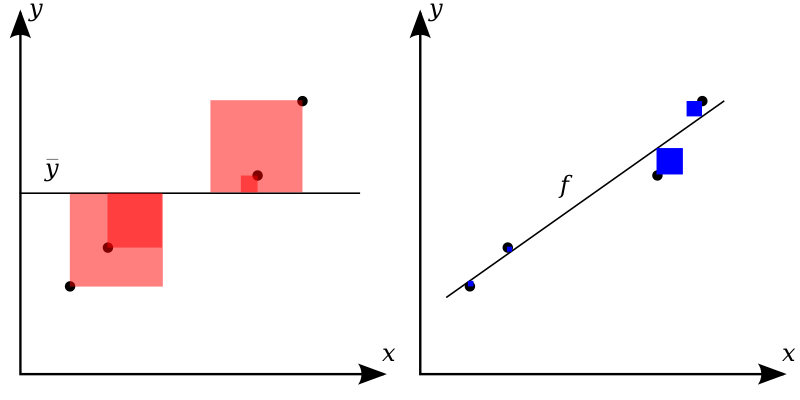
\includegraphics[width=0.75\textwidth]{../Images/Coefficient_of_Determination.png}\\
  \caption{The better the linear regression (on the right) fits the data in comparison to the simple average (on the left graph), the closer the value of $R^2$ is to one. The areas of the blue squares represent the squared residuals with respect to the linear regression. The areas of the red squares represent the squared residuals with respect to the average value (from Wikipedia)}\label{fig:CoefDetermination}
\end{figure}

A data set has values $y_i$, each of which has an associated modelled value $f_i$ (also sometimes referred to as $\hat{y}_i$). Here, the values $y_i$ are called the \emph{observed values}* and the modelled values $f_i$ are sometimes called the \emph{predicted values}.

In the following $\bar{y}$ is the mean of the observed data:

\begin{equation}
  \bar{y}=\frac{1}{n}\sum_{i=1}^n y_i
\end{equation}

where n is the number of observations.

The "variability" of the data set is measured through different sums of squares:

    $SS_\text{tot}=\sum_i (y_i-\bar{y})^2$, the total sum of squares (proportional to the sample variance);

    $SS_\text{reg}=\sum_i (f_i -\bar{y})^2$, the regression sum of squares, also called the explained sum of squares.

    $SS_\text{res}=\sum_i (y_i - f_i)^2\,$, the sum of squares of residuals, also called the residual sum of squares.

The notations $SS_{R}$ and $SS_{E}$ should be avoided, since in some texts their meaning is reversed to "Residual sum of squares" and "Explained sum of squares", respectively.

The most general definition of the coefficient of determination is

\begin{equation}
  R^2 \equiv 1 - {SS_{\rm res}\over SS_{\rm tot}}.\,
\end{equation}

\subsubsection{Relation to unexplained variance}

In a general form, $R^2$ can be seen to be related to the unexplained variance, since the second term compares the unexplained variance (variance of the model's errors) with the total variance (of the data). See fraction of variance unexplained.

\subsubsection{Adjusted $R^2$}\index{general}{coefficient of determination!adjusted}

For multiple regression, the \emph{adjusted $R^2$} value (written as $\bar{R}^2$) is often used instead of $R^2$:

\begin{equation}\label{eq:adjustedR2}
      \bar{R}^2 = 1 - (1 - R^2)\frac{n - 1}{n - p - 1}
\end{equation}

where $n$ is the sample size and $p$ is the number of independent variables.

\begin{figure}
  \centering
  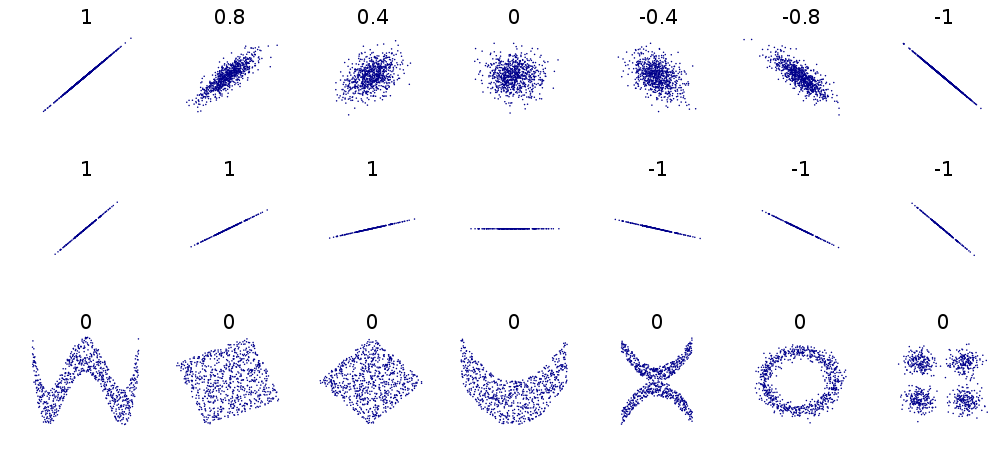
\includegraphics[width=0.75\textwidth]{../Images/Correlation_examples2.png}\\
  \caption{Several sets of (x, y) points, with the correlation coefficient of x and y for each set. Note that the correlation reflects the non-linearity and direction of a linear relationship (top row), but not the slope of that relationship (middle), nor many aspects of nonlinear relationships (bottom). N.B.: the figure in the center has a slope of 0 but in that case the correlation coefficient is undefined because the variance of Y is zero. (From: Wikipedia)}\label{fig:correlation}
\end{figure}

\subsubsection{Examples}

How large $R^2$ or $\bar{R}^2$ must be to be considered good depends on the discipline. They are usually expected to be larger in the physical sciences than it is in biology or the social sciences. In finance or marketing, it also depends on what is being modeled.

Caution: the sample correlation and $R^2$ are misleading if there is a nonlinear relationship between the independent and dependent variables!

\subsection{Rank Correlation}

If the data distribution is not normal, a different approach is necessary. In that case one can rank the set of subjects for each variable and compare the orderings. There are two commonly used methods of calculating the rank correlation. \index{general}{correlation!Spearman}
\index{general}{correlation!Kendall's $\tau$}

\begin{itemize}
  \item   \emph{Spearman's $\rho$}, which is exactly the same as the Pearson correlation coefficient $r$ calculated on the ranks of the observations.
  \item   \emph{Kendall's $\tau$} is also a rank correlation coefficient, measuring the association between two measured quantities. It is harder to calculate than Spearman's rho, but it has been argued that confidence intervals for Spearman’s rho are less reliable and less interpretable than confidence intervals for Kendall’s tau-parameters.
\end{itemize}

%\begin{itemize}
%  \item   "Regression to the mean"
%  \item   Partial correlation (comment)
%\end{itemize}

%(Lecture 11)

\section{Regression} \index{general}{regression}

We can use the method of \emph{regression} when we want to predict the value of one variable from the other.

\begin{figure}
  \centering
  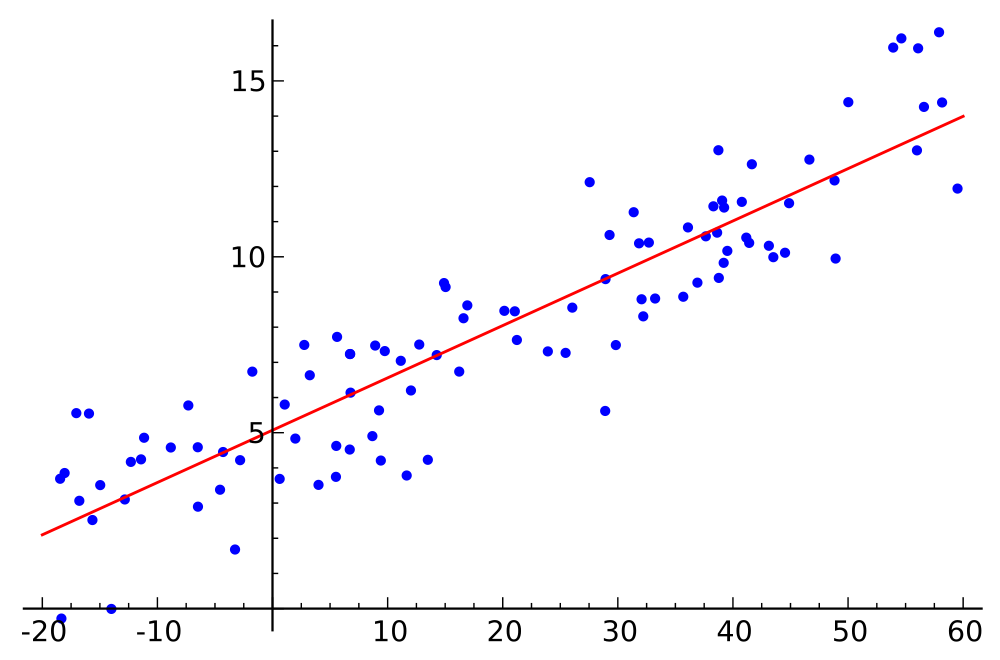
\includegraphics[width=0.75\textwidth]{../Images/Linear_regression.png}\\
  \caption{Linear regression. (From Wikipedia)}\label{fig:regression}
\end{figure}

When we search for the best-fit line to a given $(x_i,y_i)$ dataset, we are looking for the parameters $(k,d)$ which minimize the sum of the squared \emph{residuals} $\epsilon_i$ in

\begin{equation}\label{eq:simpleRegression}
  y_i = k * x_i + d + \epsilon_i
\end{equation}

where $k$ is the \emph{slope} or \emph{inclination} of the line, and $d$ the \emph{intercept}. This is in fact just the one-dimensional example of the more general technique, which is described in the next section.
Note that in contrast to the correlation, this relationship between $x$ and $y$ is no more symmetrical: it is assumed that the $x-$values are known exactly, and that all the variability lies in the residuals.

\begin{figure}
  \centering
  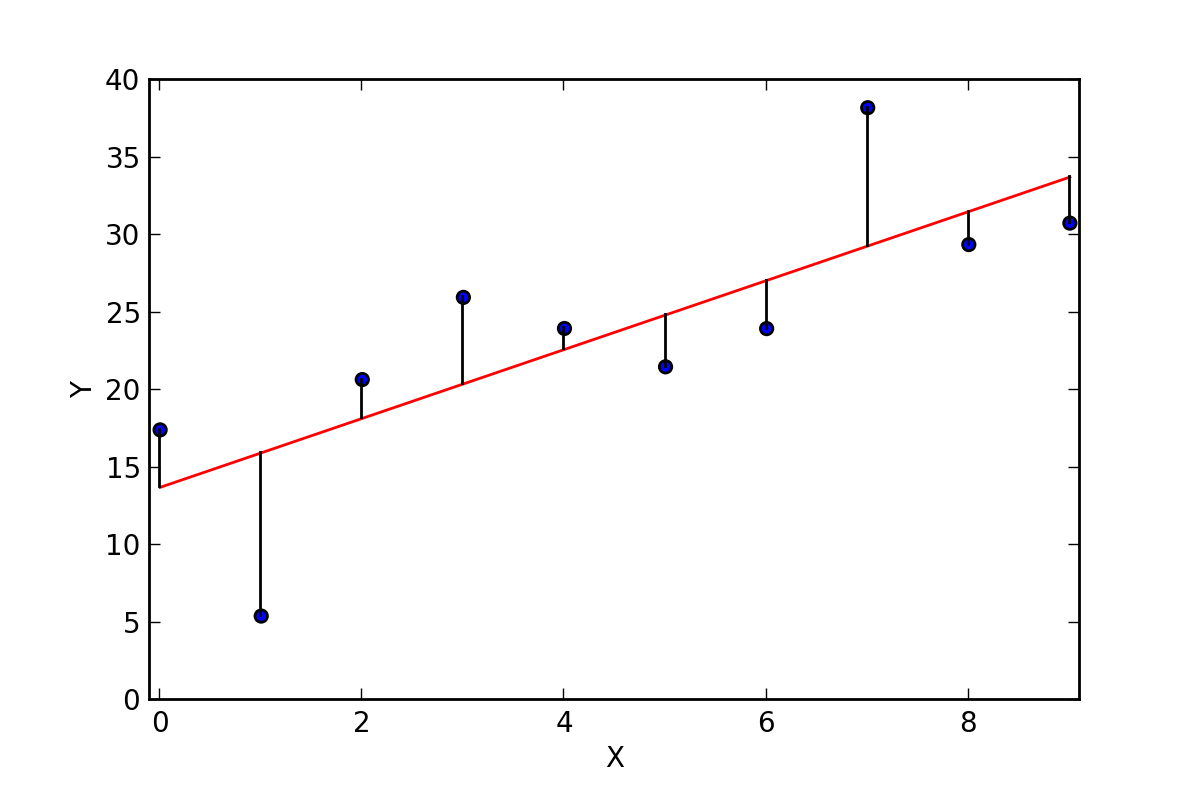
\includegraphics[width=0.75\textwidth]{../Images/residuals_linreg.png}\\
  \caption{Best-fit linear regression line (red) and residuals (black). }\label{fig:residuals}
\end{figure}


\subsection{Introduction}

\footnote{This section has been taken from Wikipedia} Given a data set $\{y_i,\, x_{i1}, \ldots, x_{ip}\}_{i=1}^n$ of $n$ statistical units, a linear regression model assumes that the relationship between the dependent variable $y_i$ and the $p$-vector of regressors $x_i$ is linear. This relationship is modelled through a \emph{disturbance term} or \emph{error variable} $\epsilon_i$, an unobserved random variable that adds noise to the linear relationship between the dependent variable and regressors. Thus the model takes the form

\begin{equation}\label{eq:regression}
   y_i = \beta_1   x_{i1} + \cdots + \beta_p x_{ip} + \varepsilon_i
   = \mathbf{x}^{\rm T}_i\boldsymbol\beta + \varepsilon_i,
   \qquad i = 1, \ldots, n,
\end{equation}

where $^T$ denotes the transpose, so that $x_i^T\beta$ is the inner product between vectors $x_i$ $\beta$.

Often these $n$ equations are stacked together and written in vector form as

\begin{equation}
  \mathbf{y} = \mathbf{X}\boldsymbol\beta + \boldsymbol\varepsilon, \,
\end{equation}

where

\begin{equation}
   \mathbf{y} = \begin{pmatrix} y_1 \\ y_2 \\ \vdots \\ y_n \end{pmatrix}, \quad
   \mathbf{X} = \begin{pmatrix} \mathbf{x}^{\rm T}_1 \\ \mathbf{x}^{\rm T}_2 \\ \vdots \\ \mathbf{x}^{\rm T}_n \end{pmatrix}
   = \begin{pmatrix} x_{11} & \cdots & x_{1p} \\
   x_{21} & \cdots & x_{2p} \\
   \vdots & \ddots & \vdots \\
   x_{n1} & \cdots & x_{np}
   \end{pmatrix}, \quad
   \boldsymbol\beta = \begin{pmatrix} \beta_1 \\ \vdots \\ \beta_p \end{pmatrix}, \quad
   \boldsymbol\varepsilon = \begin{pmatrix} \varepsilon_1 \\ \varepsilon_2 \\ \vdots \\ \varepsilon_n \end{pmatrix}.
\end{equation}

Some remarks on terminology and general use:
\begin{itemize} \index{general}{covariate} \index{general}{regressand} \index{general}{endogenous variable} \index{general}{regressor} \index{general}{exogenous variable}
  \item $y_i$  is called the \emph{regressand}, \emph{endogenous variable}, \emph{response variable}, \emph{measured variable}, or \emph{dependent variable}.  The decision as to which variable in a data set is modeled as the dependent variable and which are modeled as the independent variables may be based on a presumption that the value of one of the variables is caused by, or directly influenced by the other variables. Alternatively, there may be an operational reason to model one of the variables in terms of the others, in which case there need be no presumption of causality.
  \item $\mathbf{x}_i$ are called \emph{regressors}, \emph{exogenous variables}, \emph{explanatory variables}, \emph{covariates}, \emph{input variables}, \emph{predictor variables}, or \emph{independent variables}, but not to be confused with \emph{independent random variables}. The matrix $\mathbf{X}$ is sometimes called the \emph{design matrix}.
      \begin{itemize}
        \item Usually a constant is included as one of the regressors. For example we can take $x_{i1}=1$ for $i=1,...,n$. The corresponding element of $\beta$ is called the \emph{intercept}. Many statistical inference procedures for linear models require an intercept to be present, so it is often included even if theoretical considerations suggest that its value should be zero.
        \item Sometimes one of the regressors can be a non-linear function of another regressor or of the data, as in polynomial regression and segmented regression. The model remains linear as long as it is linear in the parameter vector $\beta$.
        \item The regressors $x_{ij}$ may be viewed either as random variables, which we simply observe, or they can be considered as predetermined fixed values which we can choose. Both interpretations may be appropriate in different cases, and they generally lead to the same estimation procedures; however different approaches to asymptotic analysis are used in these two situations.
         \end{itemize}
  \item $\boldsymbol\beta\,$ is a $p$-dimensional \emph{parameter vector}. Its elements are also called \emph{effects}, or \emph{regression coefficients}. Statistical estimation and inference in linear regression focuses on $\beta$.
  \item $\varepsilon_i\,$ is called the \emph{error term}, \emph{disturbance term}, or \emph{noise}. This variable captures all other factors which influence the dependent variable $y_i$ other than the regressors $x_i$. The relationship between the error term and the regressors, for example whether they are correlated, is a crucial step in formulating a linear regression model, as it will determine the method to use for estimation.
  \item If $i=1$ and $p=1$ in Eq.\ref{eq:regression}, we have a \emph{simple linear regression}, corresponding to Eq.\ref{eq:simpleRegression}. If $i>1$ we talk about \emph{multilinear regression} \index{general}{regression!multilinear} or \emph{multiple linear regression} \index{general}{regression!multiple linear|see{regression!multilinear}}.

\end{itemize}
\emph{Example}. Consider a situation where a small ball is being tossed up in the air and then we measure its heights of ascent $h_i$ at various moments in time $t_i$. Physics tells us that, ignoring the drag, the relationship can be modelled as
:

\begin{equation}
 h_i = \beta_1 t_i + \beta_2 t_i^2 + \varepsilon_i,
\end{equation}

where $\beta_1$ determines the initial velocity of the ball, $\beta_2$ is proportional to the standard gravity, and $\epsilon_i$ is due to measurement errors. Linear regression can be used to estimate the values of $\beta_1$ and $\beta_2$ from the measured data. This model is non-linear in the time variable, but it is linear in the parameters $\beta_1$ and $\beta_2$; if we take regressors $\mathbf{x}_i = (x_{i1},x_{i2}) = (t_i,t_i^2)$, the model takes on the standard form
:
 $h_i = \mathbf{x}^{\rm T}_i\boldsymbol\beta + \varepsilon_i.$

\subsection{Assumptions}

To use the technique of linear regression, five assumptions should be fulfilled:

\begin{enumerate}
  \item The errors in the data values (i.e. the deviations from average) are independent from one another.
  \item The model must be appropriate. (A linear regression does not properly describe a quadratic curve.)
  \item The \emph{independent variables} (i.e. $x$) are exactly known.
  \item The variance of the \emph{dependent variable} (i.e. $y$) is the same for all values of $x$.
  \item The distribution of $y$ is approximately normal for all values of $x$.
\end{enumerate}

\begin{figure}
  \centering
  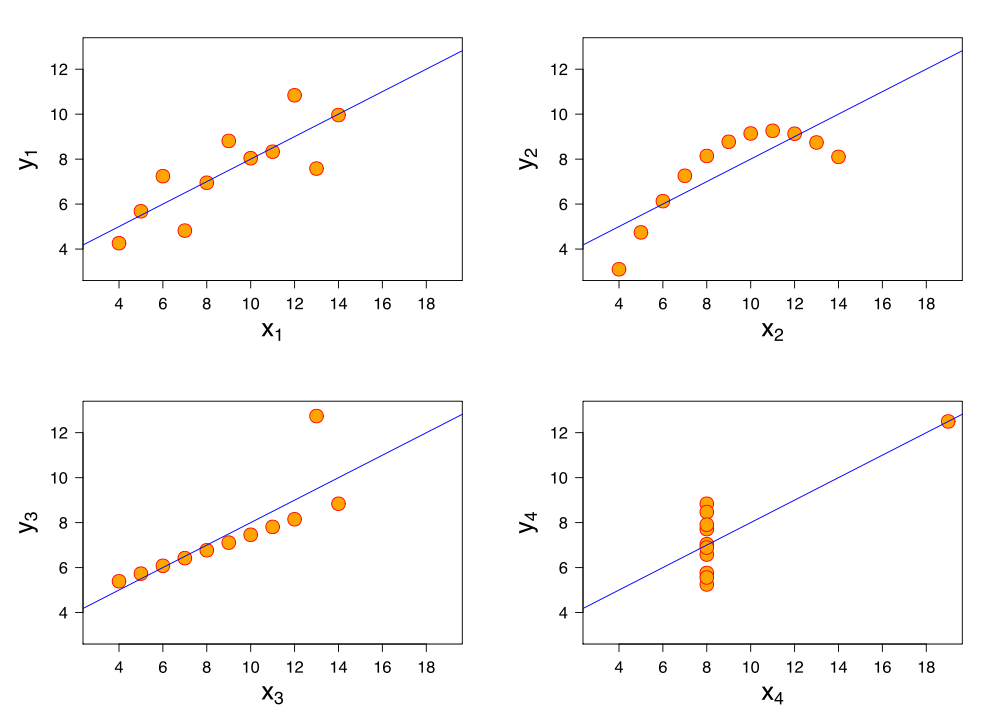
\includegraphics[width=0.75\textwidth]{../Images/Anscombes_quartet.png}\\
  \caption{The sets in the \emph{Anscombe's quartet} have the same linear regression line but are themselves very different.}
\end{figure}

\PyImg "multivariate.py" (p \pageref{py:multivariate}): Analysis of multivariate data (regression, correlation).
\index{python}{multivariate}

\begin{figure}
  \centering
  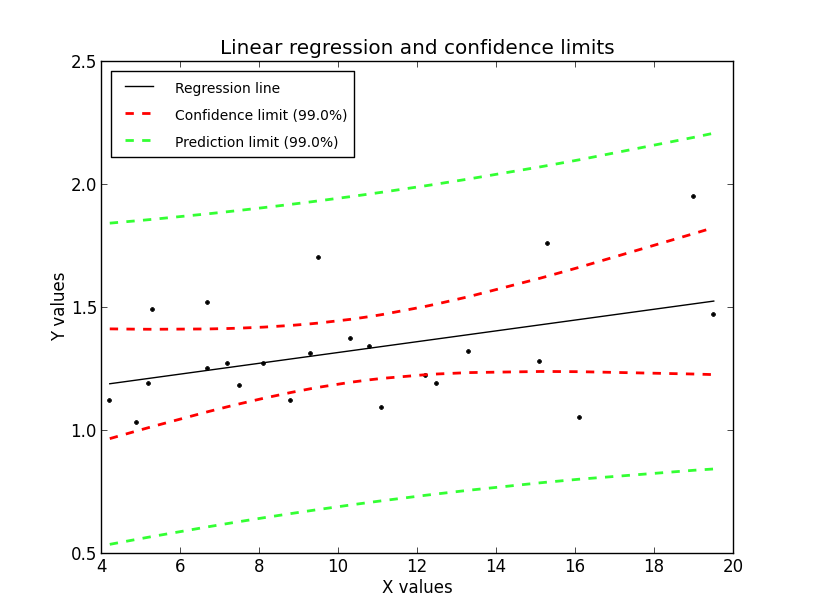
\includegraphics[width=0.75\textwidth]{../Images/regression_wLegend.png}\\
  \caption{Regression, with confidence intervals for the mean, as well as for the predicted data. The red dotted line shows the confidence interval for the mean; and the green dotted line the confidence interval for predicted data. (This can be compared to the standard error and the standard deviation for a population.)} \label{fig:regline}
\end{figure}

Since to my knowledge there exists no program in the Python standard library (or numpy, scipy) to calculate the confidence intervals for a regression line, I include my corresponding program \emph{lineFit.py} \ref{py:fitLine}. The output of this program is shown in Figure \ref{fig:regline}. This program also shows how Python programs intended for distribution should be documented.

\PyImg "fitLine.py" (p \pageref{py:fitLine}): Linear regression fit.
\index{python}{fitLine}

\section{Exercises}

\begin{enumerate}
  \item \textbf{Correlation}

    Read in the data for the average yearly temperature at the Sonnblick, from     \emph{https://github.com/thomas-haslwanter/statsintro/blob/master/Data/data\_others/AvgTemp.xls}
    Calculate the Pearson and Spearman correlation, and Kendall's tau, for the temperature vs. year.

  \item \textbf{Regression}

    For the same data, calculate the yearly increase in temperature, assuming a linear increase with time.
    Is this increase significant?

  \item \textbf{Normality Check}

    For the data from the regression model, check if the model is ok by testing if the residuals are normally distributed (e.g. by using the Kolmogorov-Smirnov test)

\end{enumerate}



\chapter{Relation Between Several Variables}

When we have two groups, we can ask the question: "Are they different?" The answer is provided by hypothesis tests: by a \emph{t-test} if the data are normally distributed, or by a \emph{Mann-Whitney test} otherwise. If we want to go one step further and predict the value of one variable from another, we have to use the technique of \emph{linear regression}.

So what happens when we have more than two groups?

To answer the question "Are they different?" for more than two groups, we have to use the \emph{Analysis of Variance (ANOVA)-test} for data where the residuals are normally distributed. If this condition is not fulfilled, the \emph{Kruskal-Wallis Test} has to be used.

What should we do if we have paired data?

If we have matched pairs for two groups, and the differences are not normally distributed, we can use the \emph{Wilcoxon signed rank sum test}. The rank test for more than two groups of matched data is the \emph{Friedman test}\index{general}{test!Friedman}.\footnote{It may be worth mentioning that Thom Baguley suggested the following: Where one-way repeated measures ANOVA is not appropriate, rank transformation followed by ANOVA will provide a more robust test with greater statistical power than the Friedman test.}

An example for the application of the Friedman test: Ten professional piano players are blindfolded, and are asked to judge the quality of three different pianos. Each player rates each piano on a scale of 1 to 10 (1 being the lowest possible grade, and 10 the highest possible grade). The null hypothesis is that all three pianos rate equally. To test the null hypothesis, the Friedman test is used on the ratings of the ten piano players.

And if we want to and predict the value of one variable \emph{many} other variables, linear regression has to be replaced by of \emph{multilinear regression} \index{general}{regression!multilinear}, sometimes also referred to as \emph{multiple linear regression}.

\section{Two-way ANOVA} \label{sec:anovaTwoWay} \index{general}{ANOVA, two-way} \index{general}{test!ANOVA}

Compared to one-way ANOVAs, the analysis with two-way ANOVAs has a new element. We can look not only if each of the factors is significant; we can also check if the \emph{interaction} of the factors has a significant influence on the distribution of the data. For sticking to the example above, if only women with treatment B get healthy, we have a significant interaction effect between "gender" and "treatment".

\PyImg "anovaTwoway.py" (p \pageref{py:anovaTwoway}): Two-way Analysis of Variance (ANOVA).
\index{python}{anovaTwoway}

\begin{verbatim}
                        df  sum_sq mean_sq        F    PR(>F)
  C(fetus)               2  324.00  162.00  2113.10  1.05e-27
  C(observer)            3    1.19    0.39     5.21  6.497-03
  C(fetus):C(observer)   6    0.56    0.09     1.22  3.29e-01
  Residual              24    1.84    0.07      NaN       NaN
\end{verbatim}

\section{Multilinear Regression} \index{general}{regression!multilinear}

If you have truly independent variables, \emph{multilinear regression} is a straitforward extension of the simple linear regression. However, if your variables may be related to each other, you have to proceed much more carefully. For example, you may want to investigate how the prevalence of some disease correlates with age and with income: if you do so, you have to keep in mind that age and income are most likely correlated! For details, \cite{Kaplan2009} gives a good introduction to that topic. Also, check out the chapter on Modeling.

\PyImg "mult\_regress.py" (p \pageref{py:mult_regress}): Multiple regression example.
\index{python}{multipleRegression}
\chapter{ Statistical Models } \index{general}{statistical modeling}

\section{Model language}
The mini-language commonly used now in statistics to describe formulas was first used in the languages $R$ and $S$, but is now also available in Python through the module \emph{patsy}.

For instance, if we have some variable $y$, and we want to regress it against some other variables $x, a, b$, and the interaction of a and b, then we simply write

\begin{equation}
    y \sim x + a + b + a:b
\end{equation}

The symbols in Table \ref{tab:syntax} are used on the right hand side to denote different interactions.

\begin{table}
  \centering
  \footnotesize{
  \begin{tabular}{ p{2cm} p{9cm} }
     Operator & Meaning \\
     \hline
    $\sim $ &	Separate the left-hand side from the right-hand side. If omitted, formula is assumed right-hand side only. \\
    + &	Combines terms on either side (set union). \\
    - &	Removes terms on the right from set of terms on the left (set difference). \\
    * &	a*b is shorthand for the expansion a + b + a:b. \\
    / &	a/b is shorthand for the expansion a + a:b. It is used when b is nested within a (e.g., states and counties) \\
    : &	Computes the interaction between terms on the left and right. \\
    ** & Takes a set of terms on the left and an integer n on the right and computes the * of that set of terms with itself n times.\\
     \hline
  \end{tabular}
  }
  \caption{Formula sytax}
\end{table}\label{tab:syntax}

A complete set of the description is found under \cite{patsy}

\subsection{Design Matrix}

\subsubsection{Definition}
A very general definition of a regression model is the following:

\begin{equation}
  y =f(x,\epsilon)
\end{equation}
In the case of a linear regression model, the function f is simply the affine function, and the model can be rewritten as:
\begin{equation}
    y=X\beta+ \epsilon,
\end{equation}
$Y$ is a vector of dimension $(n \times 1)$ and is called the \emph{endogenous variable}, the \emph{Design matrix} $X$ is a matrix of dimension $(n \times k)$ where each column is an explanatory variable, and $\epsilon$ is the error term. $\beta$ is the vector of dimension $(k \times 1)$ and contains the parameters we want to estimate.

\subsubsection{Examples}
\paragraph{Simple Regression}
Example of \emph{simple linear regression} with 7 observations.
Suppose there are 7 data points $\left\{ {{y_i},{x_i}} \right\}$, where $i=1,2,…,7$. The simple linear regression model is

\begin{equation}
  y_i = \beta_0 + \beta_1 x_i +\epsilon_i, \,
\end{equation}

where $\beta_0$ is the y-intercept and $\beta_1$ is the slope of the regression line. This model can be represented in matrix form as

\begin{equation}
  \begin{bmatrix}y_1 \\ y_2 \\ y_3 \\ y_4 \\ y_5 \\ y_6 \\ y_7 \end{bmatrix}
  =
  \begin{bmatrix}1 & x_1  \\1 & x_2  \\1 & x_3  \\1 & x_4  \\1 & x_5  \\1 & x_6 \\ 1 & x_7  \end{bmatrix}
  \begin{bmatrix} \beta_0 \\ \beta_1  \end{bmatrix}
  +
  \begin{bmatrix} \epsilon_1 \\ \epsilon_2 \\ \epsilon_3 \\ \epsilon_4 \\ \epsilon_5 \\ \epsilon_6 \\ \epsilon_7 \end{bmatrix}
\end{equation}
where the first column of ones in the design matrix represents the y-intercept term while the second column is the x-values associated with the y-value.

\paragraph{Multiple Regression} \index{general}{regression!multiple}
Example of \emph{multiple regression} with covariates (i.e. independent variables) $w_i$ and $x_i$.
Again suppose that the data are 7 observations, and for each observed value to be predicted ($y_i$), there are two covariates that were also observed $w_i$ and $x_i$. The model to be considered is
\begin{equation}
  y_i = \beta_0 + \beta_1 w_i + \beta_2 x_i + \epsilon_i
\end{equation}
This model can be written in matrix terms as

\begin{equation}
  \begin{bmatrix}y_1 \\ y_2 \\ y_3 \\ y_4 \\ y_5 \\ y_6 \\ y_7 \end{bmatrix} =
    \begin{bmatrix} 1 & w_1 & x_1  \\1 & w_2 & x_2  \\1 & w_3 & x_3  \\1 & w_4 & x_4  \\1 & w_5 & x_5  \\1 & w_6 & x_6 \\ 1& w_7  & x_7  \end{bmatrix}
    \begin{bmatrix} \beta_0 \\ \beta_1 \\ \beta_2  \end{bmatrix}
    +
    \begin{bmatrix} \epsilon_1 \\ \epsilon_2 \\ \epsilon_3 \\ \epsilon_4 \\ \epsilon_5 \\ \epsilon_6 \\ \epsilon_7 \end{bmatrix}
\end{equation}

\paragraph{One-way ANOVA (Cell Means Model)}
Example with a one-way analysis of variance (ANOVA) with 3 groups and 7 observations. The given data set has the first three observations belonging to the first group, the following two observations belong to the second group and the final two observations are from the third group.
If the model to be fit is just the mean of each group, then the model is

\begin{equation}
  y_{ij} = \mu_i + \epsilon_{ij}
\end{equation}

which can be written

\begin{equation}
  \begin{bmatrix}y_1 \\ y_2 \\ y_3 \\ y_4 \\ y_5 \\ y_6 \\ y_7 \end{bmatrix} =
  \begin{bmatrix}1 & 0 & 0 \\1 &0  &0 \\ 1 & 0 & 0 \\  0 & 1 & 0 \\  0 & 1 & 0 \\  0 & 0 & 1 \\  0 & 0 & 1\end{bmatrix}
  \begin{bmatrix}\mu_1 \\ \mu_2 \\ \mu_3  \end{bmatrix}
  +
  \begin{bmatrix} \epsilon_1 \\ \epsilon_2 \\ \epsilon_3 \\ \epsilon_4 \\ \epsilon_5 \\ \epsilon_6 \\ \epsilon_7 \end{bmatrix}
\end{equation}
It should be emphasized that in this model $\mu_i$ represents the mean of the $i$th group.

\paragraph{One-way ANOVA (offset from reference group)}
The ANOVA model could be equivalently written as each group parameter $\tau_i$ being an offset from some overall reference.  Typically this reference point is taken to be one of the groups under consideration. This makes sense in the context of comparing multiple treatment groups to a control group and the control group is considered the "reference". In this example, group 1 was chosen to be the reference group. As such the model to be fit is:
\begin{equation}
  y_{ij} = \mu + \tau_i + \epsilon_{ij}
\end{equation}
with the constraint that $\tau_1$ is zero.

\begin{equation}
  \begin{bmatrix}y_1 \\ y_2 \\ y_3 \\ y_4 \\ y_5 \\ y_6 \\ y_7 \end{bmatrix} =
  \begin{bmatrix}1 &0 &0 \\1 &0  &0 \\ 1 & 0 & 0 \\ 1 & 1 & 0 \\ 1 & 1 & 0 \\ 1 & 0 & 1 \\ 1  & 0 & 1\end{bmatrix}
  \begin{bmatrix}\mu \\  \tau_2 \\ \tau_3 \end{bmatrix}
  +
  \begin{bmatrix} \epsilon_1 \\ \epsilon_2 \\ \epsilon_3 \\ \epsilon_4 \\ \epsilon_5 \\ \epsilon_6 \\ \epsilon_7 \end{bmatrix}
\end{equation}
In this model $\mu$ is the mean of the reference group and $\tau_i$ is the difference from group $i$ to the reference group. $\tau_1$ and is not included in the matrix because its difference from the reference group (itself) is necessarily zero.
\subsection{Example: Program Effectiveness}

Using data from Spector and Mazzeo (1980), we estimate a linear regression model with statsmodels.

\lstinputlisting[label=py:regSpector,caption=regSpector.py, language=Python]{C:/Users/p20529/Documents/Teaching/Master_FH/Stats/dist/Code/regSpector.py}
\index{python}{linear regression model}

\section{Assumptions}
Standard linear regression models with standard estimation techniques make a number of assumptions about the predictor variables, the response variables and their relationship.  Numerous extensions have been developed that allow each of these assumptions to be relaxed (i.e. reduced to a weaker form), and in some cases eliminated entirely.  Some methods are general enough that they can relax multiple assumptions at once, and in other cases this can be achieved by combining different extensions.  Generally these extensions make the estimation procedure more complex and time-consuming, and may also require more data in order to get an accurate model.

The following are the major assumptions made by standard linear regression models with standard estimation techniques (e.g. ordinary least squares):

\begin{itemize}
  \item \textbf{Weak exogeneity}.  This essentially means that the predictor variables $x$ can be treated as fixed values, rather than random variables.  This means, for example, that the predictor variables are assumed to be error-free, that is they are not contaminated with measurement errors. Although not realistic in many settings, dropping this assumption leads to significantly more difficult errors-in-variables models.

  \item \textbf{Linearity}.  This means that the mean of the response variable is a linear combination of the parameters (regression coefficients) and the predictor variables.  Note that this assumption is much less restrictive than it may at first seem.  Because the predictor variables are treated as fixed values (see above), linearity is really only a restriction on the parameters.  The predictor variables themselves can be arbitrarily transformed, and in fact multiple copies of the same underlying predictor variable can be added, each one transformed differently.  This trick is used, for example, in polynomial regression, which uses linear regression to fit the response variable as an arbitrary polynomial function (up to a given rank) of a predictor variable. This makes linear regression an extremely powerful inference method.  In fact, models such as polynomial regression are often "too powerful", in that they tend to overfit the data.  As a result, some kind of regularization must typically be used to prevent unreasonable solutions coming out of the estimation process.  Common examples are ridge regression and lasso regression.  Bayesian linear regression can also be used, which by its nature is more or less immune to the problem of overfitting. (In fact, ridge regression and lasso regression can both be viewed as special cases of Bayesian linear regression, with particular types of prior distributions placed on the regression coefficients.)

  \item \textbf{Constant variance} (aka \emph{homoscedasticity}).  This means that different response variables have the same variance in their errors, regardless of the values of the predictor variables. In practice this assumption is invalid (i.e. the errors are heteroscedastic) if the response variables can vary over a wide scale. In order to determine for heterogeneous error variance, or when a pattern of residuals violates model assumptions of homoscedasticity (error is equally variable around the 'best-fitting line' for all points of x), it is prudent to look for a "fanning effect" between residual error and predicted values. This is to say there will be a systematic change in the absolute or squared residuals when plotted against the predicting outcome. Error will not be evenly distributed across the regression line. Heteroscedasticity will result in the averaging over of distinguishable variances around the points to get a single variance that is inaccurately representing all the variances of the line. In effect, residuals appear clustered and spread apart on their predicted plots for larger and smaller values for points along the linear regression line, and the mean squared error for the model will be wrong. Typically, for example, a response variable whose mean is large will have a greater variance than one whose mean is small. For example, a given person whose income is predicted to be \$100,000 may easily have an actual income of \$80,000 or \$120,000 (a standard deviation]] of around \$20,000), while another person with a predicted income of \$10,000 is unlikely to have the same \$20,000 standard deviation, which would imply their actual income would vary anywhere between -\$10,000 and \$30,000. (In fact, as this shows, in many cases – often the same cases where the assumption of normally distributed errors fails – the variance or standard deviation should be predicted to be proportional to the mean, rather than constant.) Simple linear regression estimation methods give less precise parameter estimates and misleading inferential quantities such as standard errors when substantial heteroscedasticity is present. However, various estimation techniques (e.g. weighted least squares and heteroscedasticity-consistent standard errors) can handle heteroscedasticity in a quite general way. Bayesian linear regression techniques can also be used when the variance is assumed to be a function of the mean. It is also possible in some cases to fix the problem by applying a transformation to the response variable (e.g. fit the logarithm of the response variable using a linear regression model, which implies that the response variable has a log-normal distribution rather than a normal distribution).

  \item \textbf{Independence of errors}.  This assumes that the errors of the response variables are uncorrelated with each other. (Actual statistical independence is a stronger condition than mere lack of correlation and is often not needed, although it can be exploited if it is known to hold.) Some methods (e.g. generalized least squares) are capable of handling correlated errors, although they typically require significantly more data unless some sort of regularization is used to bias the model towards assuming uncorrelated errors. Bayesian linear regression is a general way of handling this issue.

  \item \textbf{Lack of multicollinearity in the predictors}.  For standard least squares estimation methods, the design matrix $X$ must have full column rank $p$; otherwise, we have a condition known as multicollinearity in the predictor variables.  This can be triggered by having two or more perfectly correlated predictor variables (e.g. if the same predictor variable is mistakenly given twice, either without transforming one of the copies or by transforming one of the copies linearly). It can also happen if there is too little data available compared to the number of parameters to be estimated (e.g. fewer data points than regression coefficients). In the case of multicollinearity, the parameter vector $\beta$ will be non-identifiable, it has no unique solution.  At most we will be able to identify some of the parameters, i.e. narrow down its value to some linear subspace of $R^p$. Methods for fitting linear models with multicollinearity have been developed. Note that the more computationally expensive iterated algorithms for parameter estimation, such as those used in generalized linear models, do not suffer from this problem — and in fact it's quite normal to when handling categorical data|categorically-valued predictors to introduce a separate indicator variable predictor for each possible category, which inevitably introduces multicollinearity.
\end{itemize}
Beyond these assumptions, several other statistical properties of the data strongly influence the performance of different estimation methods:

\begin{itemize}
  \item The statistical relationship between the error terms and the regressors plays an important role in determining whether an estimation procedure has desirable sampling properties such as being unbiased and consistent.
  \item The arrangement, or probability distribution of the predictor variables $x$ has a major influence on the precision of estimates of $\beta$. Sampling and design of experiments are highly-developed subfields of statistics that provide guidance for collecting data in such a way to achieve a precise estimate of $\beta$.
\end{itemize}

\subsection{Interpretation}

A fitted linear regression model can be used to identify the relationship between a single predictor variable $x_j$ and the response variable $y$ when all the other predictor variables in the model are “held fixed”. Specifically, the interpretation of $\beta_j$ is the expected change in $y$ for a one-unit change in $x_j$ when the other covariates are held fixed—that is, the expected value of the partial derivative of $y$ with respect to $x_j$. This is sometimes called the ''unique effect'' of $x_j$ on ''y''. In contrast, the ''marginal effect'' of $x_j$ on $y$ can be assessed using a correlation coefficient or simple linear regression model relating $x_j$ to $y$; this effect is the total derivative of $y$ with respect to $x_j$.

Care must be taken when interpreting regression results, as some of the regressors may not allow for marginal changes (such as dummy variables, or the intercept term), while others cannot be held fixed (recall the example from the introduction: it would be impossible to “hold $t_j$ fixed” and at the same time change the value of $t_i^2$.

It is possible that the unique effect can be nearly zero even when the marginal effect is large. This may imply that some other covariate captures all the information in $x_j$, so that once that variable is in the model, there is no contribution of $x_j$ to the variation in $y$. Conversely, the unique effect of $x_j$ can be large while its marginal effect is nearly zero. This would happen if the other covariates explained a great deal of the variation of $y$, but they mainly explain variation in a way that is complementary to what is captured by $x_j$. In this case, including the other variables in the model reduces the part of the variability of $y$ that is unrelated to $x_j$, thereby strengthening the apparent relationship with $x_j$.

The meaning of the expression “held fixed” may depend on how the values of the predictor variables arise. If the experimenter directly sets the values of the predictor variables according to a study design, the comparisons of interest may literally correspond to comparisons among units whose predictor variables have been “held fixed” by the experimenter. Alternatively, the expression “held fixed” can refer to a selection that takes place in the context of data analysis. In this case, we “hold a variable fixed” by restricting our attention to the subsets of the data that happen to have a common value for the given predictor variable. This is the only interpretation of “held fixed” that can be used in an observational study.

The notion of a “unique effect” is appealing when studying a complex system where multiple interrelated components influence the response variable. In some cases, it can literally be interpreted as the causal effect of an intervention that is linked to the value of a predictor variable. However, it has been argued that in many cases multiple regression analysis fails to clarify the relationships between the predictor variables and the response variable when the predictors are correlated with each other and are not assigned following a study design.


\lstinputlisting[label=py:modeling,caption=modeling.py, language=Python]{C:/Users/p20529/Documents/Teaching/Master_FH/Stats/dist/Code/modeling.py}
\index{python}{modeling}


\section{Evaluation of for Linear Regression Models}

One of the things that intimidated me about statistical modeling is the
deluge of expressions that appear when you run a modeling command. In the
following I will try to explain the most common parameters that you are
going to encounter when working with Linear Regression Models.


\subsection{Definitions for Regression with Intercept}

$n$ is the number of observations, $p$ is the number of regression parameters. For example, if you fit a straight line, $p=2$.
In the following $\hat{y}_i$ will indicate the fitted model values, and $\bar{y}$ will indicate the mean.

\begin{itemize}
  \item $SSM = \sum_{i=1}^n (\hat{y}_i-\bar{y})^2$ is the \emph{Sum of Square for Model}, or the sum of squares for the regression.
  \item $SSE = \sum_{i=1}^n (y_i-\hat{y}_i)^2$ is the \emph{sum of Squares for Error}, or the sum of squares for the residuals.
  \item $SST = \sum_{i=1}^n (y_i-\bar{y})^2$ is the \emph{Sum of Squares Total}, and is equivalent to the sample variance multiplied by $n-1$.
\end{itemize}

For multiple regression models, $SSM + SSE = SST$

\begin{itemize}
  \item $DFM = p - 1$ is the \emph{(Corrected) Degrees of Freedom for Model}. (The "-1" comes from the fact that we are only interested in the correlation, not in the absolute offset of the data.
  \item $DFE = n - p$ is the \emph{Degrees of Freedom for Error}
  \item $DFT = n - 1$ is the \emph{(Corrected) Degrees of Freedom Total}. The Horizontal line regression is the null hypothesis model.
\end{itemize}

For multiple regression models with intercept, DFM + DFE = DFT.

\begin{itemize}
  \item $MSM = SSM / DFM$ : \emph{Mean of Squares for Model}
  \item $MSE = SSE / DFE$ : \emph{Mean of Squares for Error}. MSE is an unbiased estimate for $\sigma^2$ for multiple regression models.
  \item $MST = SST / DFT$ : \emph{Mean of Squares Total}, which is the sample variance of the y-variable.
\end{itemize}

\subsection{The $R^2$ Value}

The $R^2$ value indicates the proportion of variation in the y-variable that is due to variation in the x-variables. For simple linear regression, the $R^2$ value is the square of the sample correlation $r_{xy}$. For multiple linear regression with intercept (which includes simple linear regression), the $R^2$ value is defined as

\begin{equation}
  R^2 = \frac{SSM}{SST}
\end{equation}

Many researchers prefer the adjusted $\bar{R}^2$ value (Eq \ref{eq:adjustedR2}), which is penalized for having a large number of parameters in the model:

Here is the logic behind the definition of $\bar{R}^2$:
$R^2$ is defined as $R^2 = 1 - SSE/SST$ or $1 - R^2 = SSE/SST$. To take into account the number of regression parameters $p$, define the adjusted R-squared value as
\begin{equation}
  1- \bar{R}^2 = \frac{Variance for Error}{Variance Total}
\end{equation}

where \emph{Variance for Error }is estimated by $SSE/DFE = SSE/(n-p)$, and \emph{Variance Total }is estimated by $SST/DFT = SST/(n-1)$. Thus,
\begin{eqnarray}
    1 - \bar{R}^2 &=& \frac{SSE/(n - p)}{SST/(n - 1)} \\
          	&=& \frac{SSE}{SST}\frac{n - 1}{n - p}
\end{eqnarray}

    so
\begin{eqnarray}
  \bar{R}^2 &=& 1 - \frac{SSE}{SST} \frac{n - 1}{(n - p} \\
    &=& 1 - (1 - R^2)\frac{n - 1}{n - p}
\end{eqnarray}


\subsection{The F-test}

If $t_1, t_2, ... , t_m$ are independent, $N(0, \sigma^2)$ random variables, then $\sum_{i=1}^m t_i^2$ is a $\chi^2$ (chi-squared) random variable with $m$ degrees of freedom.

For a multiple regression model with intercept,
\begin{equation}
  Y_j = \alpha + \beta_1 X_{1j} + ... + \beta_n X_{nj} + \epsilon_i = \alpha + \sum_{i=1}^n \beta_i X_{ij} + \epsilon_j = E(Y_j | X) + \epsilon_j
\end{equation}

we want to test the following null hypothesis and alternative hypothesis:

        $H_0$:   $\beta_1$ = $\beta_2$ = , ... , = $\beta_n$ = 0

        $H_1$:   $\beta_j \neq 0$, for at least one value of j

This test is known as the overall \emph{F-test for regression}.

It can be shown that if $H_0$ is true and the residuals are unbiased, homoscedastic, independent, and normal:

\begin{enumerate}
  \item $SSE / \sigma^2$ has a $\chi^2$ distribution with DFE degrees of freedom.
  \item $SSM / \sigma^2$ has a $\chi^2$ distribution with DFM degrees of freedom.
  \item SSE and SSM are independent random variables.
\end{enumerate}

If $u$ is a $\chi^2$ random variable with $n$ degrees of freedom, $v$ is a $\chi^2$ random variable with $m$ degrees of freedom, and $u$ and $v$ are independent, then if $F = \frac{u/n}{v/m}$ has an F distribution with $(n,m)$ degrees of freedom.

If H0 is true,

\begin{equation}
  F = \frac{(SSM/\sigma^2)/DFM}{(SSE/\sigma^2)/DFE} = \frac{SSM/DFM}{SSE/DFE} = \frac{MSM}{MSE},
\end{equation}

has an F distribution with $(DFM, DFE)$ degrees of freedom, and is independent of $\sigma$.


\subsection{Log-Likelihood Function}

A very common approach in statistics is the idea of \emph{Maximum Likelihood} estimation. \index{general}{Maximum likelihood} The basic idea is quite different from the \emph{minimum square} approach: there, the model is constant, and the errors of the response are variable; in contrast, in the maximum likelihood approach, the data response values are regarded as constant, and the likelihood of the model is maximised.

For the Classical Linear Regression Model (with normal errors) we have

\begin{equation}
  \epsilon = y_i - \sum_{k=1}^n \beta_k x_{ik} = y_i - \mathbf{x_i^{'}} \cdot \boldsymbol\beta \; in \; N(0, \sigma^2)
\end{equation}

so the probability density is given by

\begin{equation}
  p(\epsilon_i) =  \Phi (\frac{y_i - \mathbf{x_i^{'}} \cdot \boldsymbol\beta}{\sigma})
\end{equation}

where $\Phi(z)$ is the standard normal probability distribution function. The probability of independent samples is the product of the individual probabilities

\begin{equation}
  \Pi_{total} = \prod_{i=1}^n p(\epsilon_i)
\end{equation}

The \emph{Log Likelihood function} \index{general}{log likelihood function} is defined as

\begin{eqnarray*}
  Log L &=& log(\Pi_{total}) \\
  &=& log\left[\prod_{i=1}^n \frac{1}{\sigma\sqrt{2 \pi}} \exp \left(\frac{(y_i - \mathbf{x_i^{'}} \cdot \boldsymbol\beta)^2}{2 \sigma^2}\right)\right] \\
  &=& \sum_{i=1}^n\left[log\left(\frac{1}{\sigma \sqrt{2 \pi}}\right)- \left(\frac{(y_i - \mathbf{x_i^{'}} \cdot \boldsymbol\beta)^2}{2 \sigma^2}\right)\right] \\
 &=& n log(\sigma) - n log \sqrt{2 \pi} - \frac{SSE}{2 \sigma^2}
\end{eqnarray*}

It can be shown that the maximum likelihood estimator of $\sigma^2$ is

\begin{equation}
  E(\sigma^2) = \frac{SEE}{n}
\end{equation}

With this, the maximised log likelihood is
\begin{equation}
  Max(Log L) = -\frac{n}{2} log \left(\frac{2 \pi}{n} \right) - \frac{n}{2} - \frac{n}{2} log(SSE)
\end{equation}

and the maximised likelihood is

\begin{equation}
  Max(L) = \left( \frac{2 \pi}{n} \right)^{n/2} \cdot exp(- \frac{n}{2}) \cdot (SSE)^{-n/2}
\end{equation}

\subsection{Information Content of Statistical Models}

To judge the quality of your model, you should first visually inspect the residuals. In addition, you can also use a number of numerical criteria to assess the quality of a statistical model. These criteria represent various approaches for balancing model accuracy with parsimony.

We have already encountered the $adjusted R^2$ value (Eq \ref{eq:adjustedR2}), which - in contrast to the $R^2$ value - decreases if there are too many regressors in the model.

The \emph{Akaike Information Criterion AIC} \index{general}{Akaike Information Criterion AIC}

\begin{equation}
  AIC = n * ln(SSE / n) + 2p
\end{equation}

and the Schwartz or \emph{Baysian Information Criterion BIC} \index{general}{Baysian Information Criterion BIC}

\begin{equation}
  BIC = n * ln(SSE/n) + p ln(n)
\end{equation}

are other commonly encountered criteria.

\subsubsection{Analysis of Residuals}

The \textsf{OLS} command from \textsf{statsmodels.formula.api} provides some additional information about the residuals of the model:
\begin{description}
  \item[Omnibus]     In Multiple Regression the omnibus test is an ANOVA F test on all the coefficients, that is equivalent to the multiple correlations R Square F test. The omnibus F test is an overall test that examines model fit, thus rejecting the null hypothesis implies that the suggested linear model is not significally suitable to the data.
  \item[Skewness] Sample skewness of the residuals, i.e. if they have a tail to the left or to the right. Equivalent to \textsf{stats.skew(model.resid, bias=True)}.
  \item[Kurtosis] Sample kurtosis of the residuals, i.e. the pointedness of the data distribution. For normally distributed data approximately 3. (Equivalent to \textsf{stats.kurtosis(model.resid, fisher=False, bias=True)})
  \item[Durbin-Watson] A test statistic used to detect the presence of autocorrelation (a relationship between values separated from each other by a given time lag) in the residuals.
  \item[Jarque-Bera] A goodness-of-fit test of whether sample data have the skewness and kurtosis matching a normal distribution.
\end{description}

\section{Bootstrapping} \index{general}{bootstrapping}

Another type of modelling is \emph{bootstrapping}/. Sometimes you have data describing a distribution, but do not know what type of distribution it is. So what can you do if you want to find out e.g. confidence values for the mean?

The answer is bootstrapping. Bootstrapping is a scheme of \emph{resampling}, i.e. taking additional samples repeatedly from the initial sample, to provide estimates of its variability. In a case where the distribution of the initial sample is unknown, bootstrapping is of especial help in that it provides information about the distribution.

\lstinputlisting[label=py:bootstrappin,caption=bootstrap.py, language=Python]{C:/Users/p20529/Documents/Teaching/Master_FH/Stats/dist/Code/bootstrap.py}
\index{python}{bootstrap}

\chapter{Analysis of Survival Times} \index{general}{survival times}

When analyzing survival times, different problems come up than the ones discussed so far. One question is how do we deal with subjects dropping out of a study. For example, assume that we test a new cancer drug. While some subjects die, others may believe that the new drug is not effective, and decide to drop out of the study before the study is finished.
A similar problem would be faced when we investigate how long a machine lasts before it breaks down.

\section{Survival Probabilities}

\subsection{Kaplan-Meier survival curve} \index{general}{Kaplan-Meier survival curve}

A clever way to deal with these problems is described in detail in \cite{altman99}. First, the time is subdivided into small periods. Then the likelihood is calculated that a subject survives a given period. The survival probability is given by

\begin{equation}
  p_k = p_{k-1} * \frac{r_k-f_k}{r_k}
\end{equation}

where $p_k$ is the probability to survive period $k$; $r_k$ is the number of subjects still at risk (i.e. still being followed up) immediately before the $k^{th}$ day, and $f_k$ is the number of observed failures on the day $k$. The curve describing the resulting survival probability is called \emph{life table}, \emph{survival curve}, or \emph{Kaplan-Meier curve} (see Figure \ref{fig:SurvivalCurve}).

\begin{figure}
  \centering
  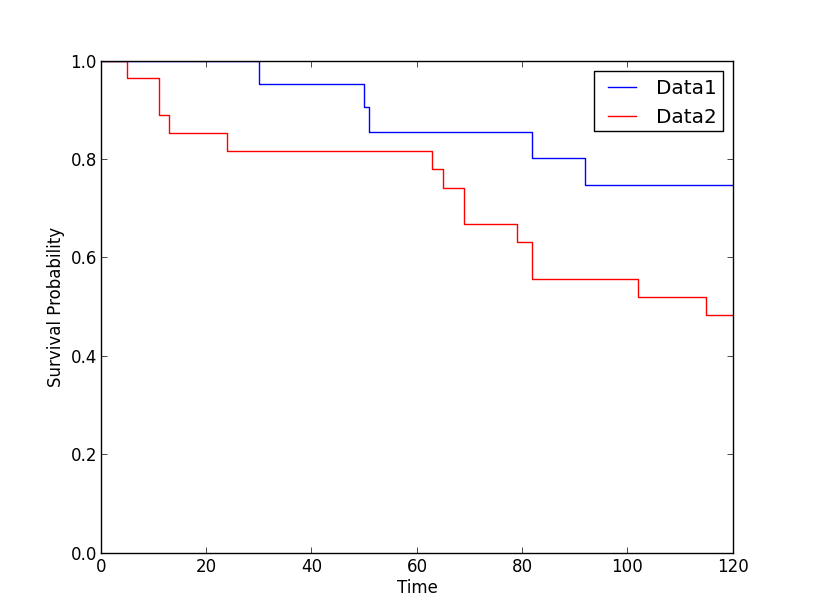
\includegraphics[width=0.5\textwidth]{../Images/Survival.png}\\
  \caption{Survival curve corresponding to a motion sickness experiment, described in more detail in \cite{altman99}, chapter 13}\label{fig:SurvivalCurve}
\end{figure}

Note that the survival curve changes only when a "failure" occurs, i.e. when a subject dies. \emph{Censored} entries, describing either when a subject drops out of the study or when the study finishes, are taken into consideration at the "failure" times, but otherwise do not affect the survival curve.

\section{Comparing Survival Curves in Two Groups} \index{general}{test!logrank}

The most common test for comparing independent groups of survival times is the \emph{logrank test}. This test is a non-parametric hypothesis test, testing the probability that both groups come from the same underlying population. Since to my knowledge this test is not yet implemented in a Python library, I have included an implementation based on the equations given by \cite{altman99} (see program \ref{py:survival}).

To explore the effect of different variables on survival, more advanced methods are required. The \emph{Cox regression model}\index{general}{Cox regression model} introduced by Cox in 1972 is used widely when it is desired to investigate several variables at the same time. For details, check \cite{altman99} or other statistic textbooks.

\lstinputlisting[label=py:survival,caption=survival.py, language=Python]{../Code/survival.py}
\index{python}{survival}


\appendix
\chapter{Appendix}

\section{Python Programs}

\lstinputlisting[label=py:gettingStarted_ipy,caption=gettingStarted\_ipy.py, language=Python]{C:/Users/p20529/Documents/Teaching/Master_FH/Stats/dist/Code3/gettingStarted_ipy.py}

\clearpage
\lstinputlisting[label=py:readZip,caption=readZip.py, language=Python]{C:/Users/p20529/Documents/Teaching/Master_FH/Stats/dist/Code3/readZip.py}

\clearpage
\lstinputlisting[label=py:pandasIntro,caption=pandasIntro.py, language=Python]{C:/Users/p20529/Documents/Teaching/Master_FH/Stats/dist/Code3/pandas_intro.py}

\clearpage
\lstinputlisting[label=py:getData,caption=getdata.py, language=Python]{C:/Users/p20529/Documents/Teaching/Master_FH/Stats/dist/Code3/getdata.py}

\clearpage
\lstinputlisting[label=py:showStats,caption=showStats.py, language=Python]{C:/Users/p20529/Documents/Teaching/Master_FH/Stats/dist/Code3/showStats.py}

\clearpage
\lstinputlisting[label=py:distributionNormal,caption=distributionNormal.py, language=Python]{C:/Users/p20529/Documents/Teaching/Master_FH/Stats/dist/Code3/distribution_normal.py}

\clearpage
\lstinputlisting[label=py:continuous,caption=Continuous,language=Python]{C:/Users/p20529/Documents/Teaching/Master_FH/Stats/dist/Code3/dist_continuous.py}

\clearpage
\lstinputlisting[label=py:discrete,caption=Discrete,language=Python]{C:/Users/p20529/Documents/Teaching/Master_FH/Stats/dist/Code3/dist_discrete.py}

\clearpage
\lstinputlisting[label=py:checkNormality,caption=checkNormality.py, language=Python]{C:/Users/p20529/Documents/Teaching/Master_FH/Stats/dist/Code3/checkNormality.py}

\clearpage
\lstinputlisting[label=py:sampleSize,caption=sampleSize.py, language=Python]{C:/Users/p20529/Documents/Teaching/Master_FH/Stats/dist/Code3/sampleSize.py}

\clearpage
\lstinputlisting[label=py:oneSample,caption=oneSample.py, language=Python]{C:/Users/p20529/Documents/Teaching/Master_FH/Stats/dist/Code3/oneSample.py}

\clearpage
\lstinputlisting[label=py:twoSample,caption=twoSample.py, language=Python]{C:/Users/p20529/Documents/Teaching/Master_FH/Stats/dist/Code3/twoSample.py}

\clearpage
\lstinputlisting[label=py:anovaOneway,caption=anovaOneway.py, language=Python]{C:/Users/p20529/Documents/Teaching/Master_FH/Stats/dist/Code3/anovaOneway.py}

\clearpage
\lstinputlisting[label=py:multipleTesting,caption=multipleTesting.py, language=Python]{C:/Users/p20529/Documents/Teaching/Master_FH/Stats/dist/Code3/multipleTesting.py}

\clearpage
\lstinputlisting[label=py:KruskalWallis,caption=KruskalWallis.py, language=Python]{C:/Users/p20529/Documents/Teaching/Master_FH/Stats/dist/Code3/KruskalWallis.py}

\clearpage
\lstinputlisting[label=py:binomial,caption=binomialTest.py, language=Python]{C:/Users/p20529/Documents/Teaching/Master_FH/Stats/dist/Code3/binomialTest.py}

\clearpage
\lstinputlisting[label=py:compGroups,caption=compGroups.py, language=Python]{C:/Users/p20529/Documents/Teaching/Master_FH/Stats/dist/Code3/compGroups.py}

\clearpage
\lstinputlisting[label=py:multivariate,caption=multivariate.py, language=Python]{C:/Users/p20529/Documents/Teaching/Master_FH/Stats/dist/Code3/multivariate.py}

\clearpage
\lstinputlisting[label=py:fitLine,caption=fitLine.py, language=Python]{C:/Users/p20529/Documents/Teaching/Master_FH/Stats/dist/Code3/fitLine.py}

\clearpage
\lstinputlisting[label=py:anovaTwoway,caption=anovaTwoway.py, language=Python]{C:/Users/p20529/Documents/Teaching/Master_FH/Stats/dist/Code3/anovaTwoway.py}

\clearpage
\lstinputlisting[label=py:mult_regress,caption=mult\_regress.py, language=Python]{C:/Users/p20529/Documents/Teaching/Master_FH/Stats/dist/Code3/mult_regress.py}

\clearpage
\lstinputlisting[label=py:regSpector,caption=regSpector.py, language=Python]{C:/Users/p20529/Documents/Teaching/Master_FH/Stats/dist/Code3/regSpector.py}

\clearpage
\lstinputlisting[label=py:modeling,caption=modeling.py, language=Python]{C:/Users/p20529/Documents/Teaching/Master_FH/Stats/dist/Code3/modeling.py}

\clearpage
\lstinputlisting[label=py:bootstrapping,caption=bootstrap.py, language=Python]{C:/Users/p20529/Documents/Teaching/Master_FH/Stats/dist/Code3/bootstrapDemo.py}

\clearpage
\lstinputlisting[label=py:survival,caption=survival.py, language=Python]{C:/Users/p20529/Documents/Teaching/Master_FH/Stats/dist/Code3/survival.py}

\clearpage

\section{Lecture Schedule}

\begin{enumerate}
  \item Introduction
  \item Basics [T]
  \item Study Design
  \item Normal Distribution [T]
  \item Other Continuous Distributions
  \item Data Analysis [T]
  \item Statistical Tests
  \item Continous Tests
  \item \textbf{Discussion of Projects}
  \item Categorical Tests
  \item Correlation [T]
  \item Regression [T]
  \item ANOVA [T]
  \item Statistical Models
  \item \textbf{Presentation of Projects}
\end{enumerate}

\section{To Do}

\begin{enumerate}
  \item What is the correct implementation of McNemar's test?
  \item Outlier detection
  \item kde
  \item Bayesian statistics
  \item Improve \emph{statistical modeling}
\end{enumerate}


\clearpage

\bibliographystyle{plainnat}
\bibliography{thomas}

\printindex{general}{Index Topics}
\printindex{python}{Python Programs}

\end{document}
% ----------------------------------------------------------------
